This section describes an alternative background estimation and likelihood fit strategy, which are determined together.

In order to describe the data, we consider three contributions to the \Mbb{} distribution:  
\begin{itemize}
  \item Signal $H\rightarrow b \bar b$ from either VBF or ggF production
  \item Resonant \zjets{} from QCD and EW production
  \item Non-resonant processes dominated by QCD multi-jet production
\end{itemize}

The shapes of the signal and \zjets{} contributions are each parametrized by a Bukin function. The non-resonant background is taken from data using a fit with an analytical function in the \Mbb{} sidebands of the signal regions and control region as described in Section~\ref{sec:nonres_alt}.
The signal strength is measured with a profile likelihood fit performed
simultaneously for all signal and control regions.  The $Z$ normalization is treated as a nuisance parameter in the fit.  The Higgs mass window, 100 \GeV$<\Mbb<$140\GeV, is blinded for the signal regions.  

%\subsubsection{Parameterization of signal and \zjets{}}
%
We parameterize the signal and \zjets{} Monte Carlo templates to smooth out the local fluctuations coming from the limited statistics using a histogrammed Bukin function. The MC templates and parametrization of signal and \zjets{} \Mbb{} distributions are shown in Figures~\ref{fig:sigpar_alt} and \ref{fig:zpar_alt}. The $\chi^2$ between simulated and fitted distributions are summarized in Table~\ref{tab:sigpar_alt}. In general, the $\Mbb$ distributions for the Higgs signal and \zjets{} are well represented by the Bukin function. The potential bias of using smoothed MC templates is studied in the full profile likelihood fit. Asimov data is built by combining the non-resonant background prediction from the background-only fit described in \ref{sec:nonres_alt} with signal and \zjets{} templates from simulation and fitted with the same non-resonant background function and the smoothed MC templates to test closure. Perfect closure is obtained with $\mu_{H}=1$ and $\mu_{Z}=1$, as injected in the Asimov data.  Therefore we conclude that the parameterized templates produce no significant bias.  The likelihood fit is described in detail later in this section.

 
\begin{figure}[htbp]
  \centering    
 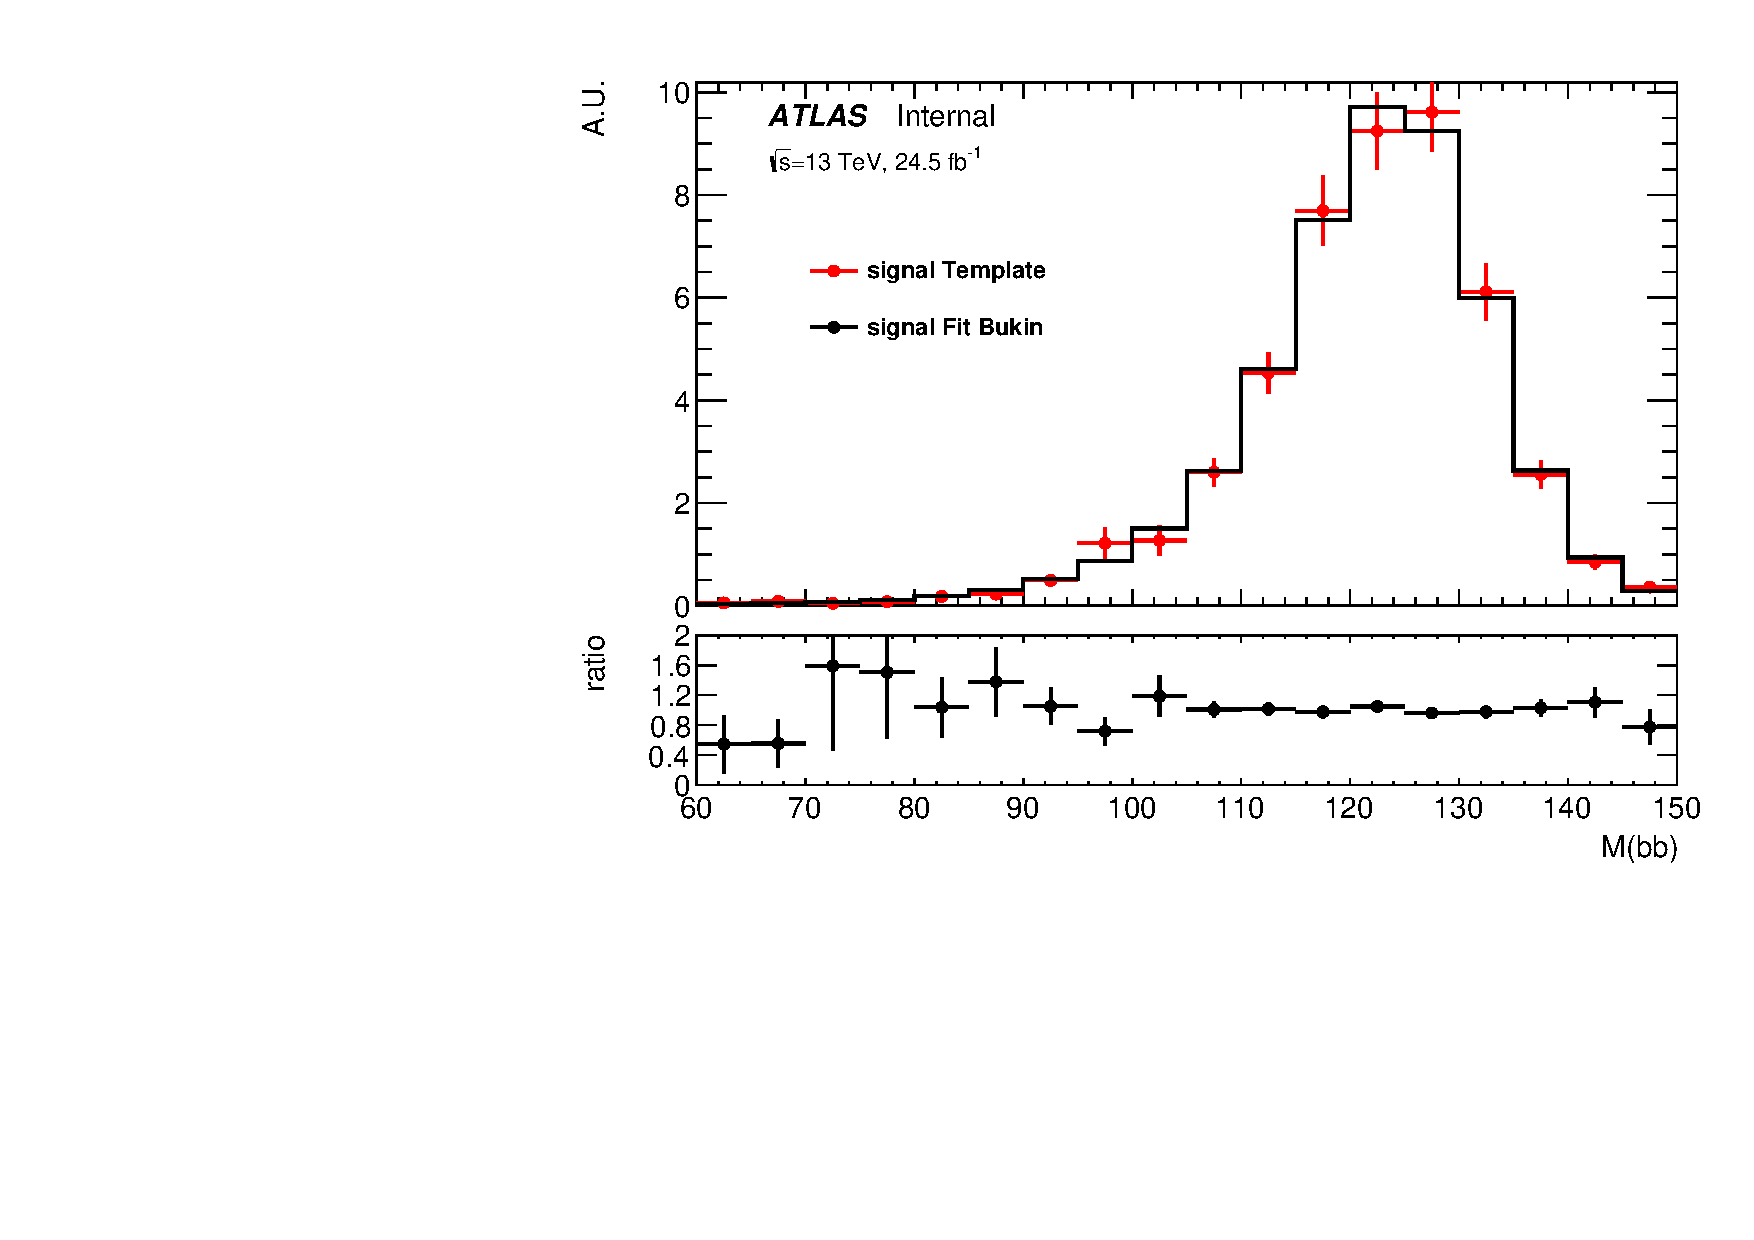
\includegraphics[width=0.24\textwidth]{figures_alt/sig_2cen_SRI.pdf}
 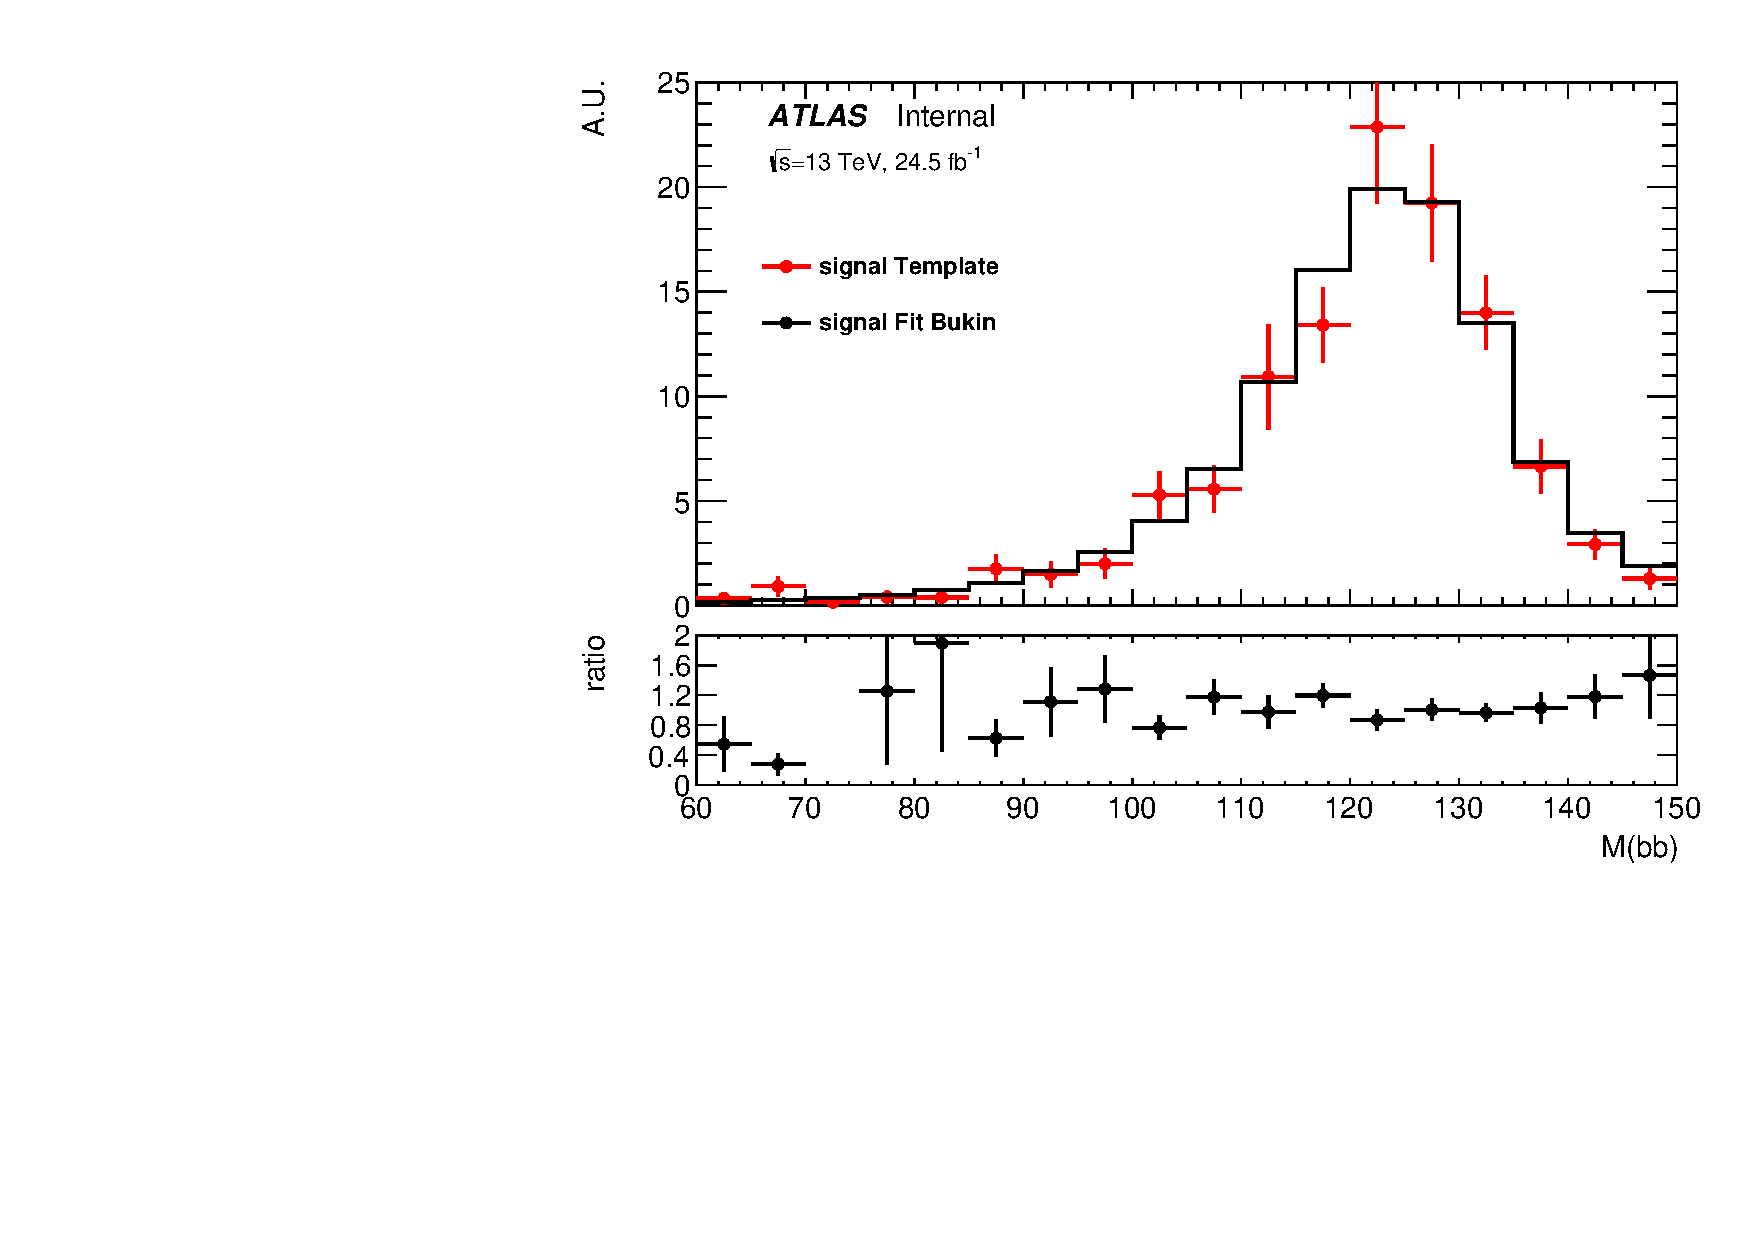
\includegraphics[width=0.24\textwidth]{figures_alt/sig_2cen_SRII.pdf}
 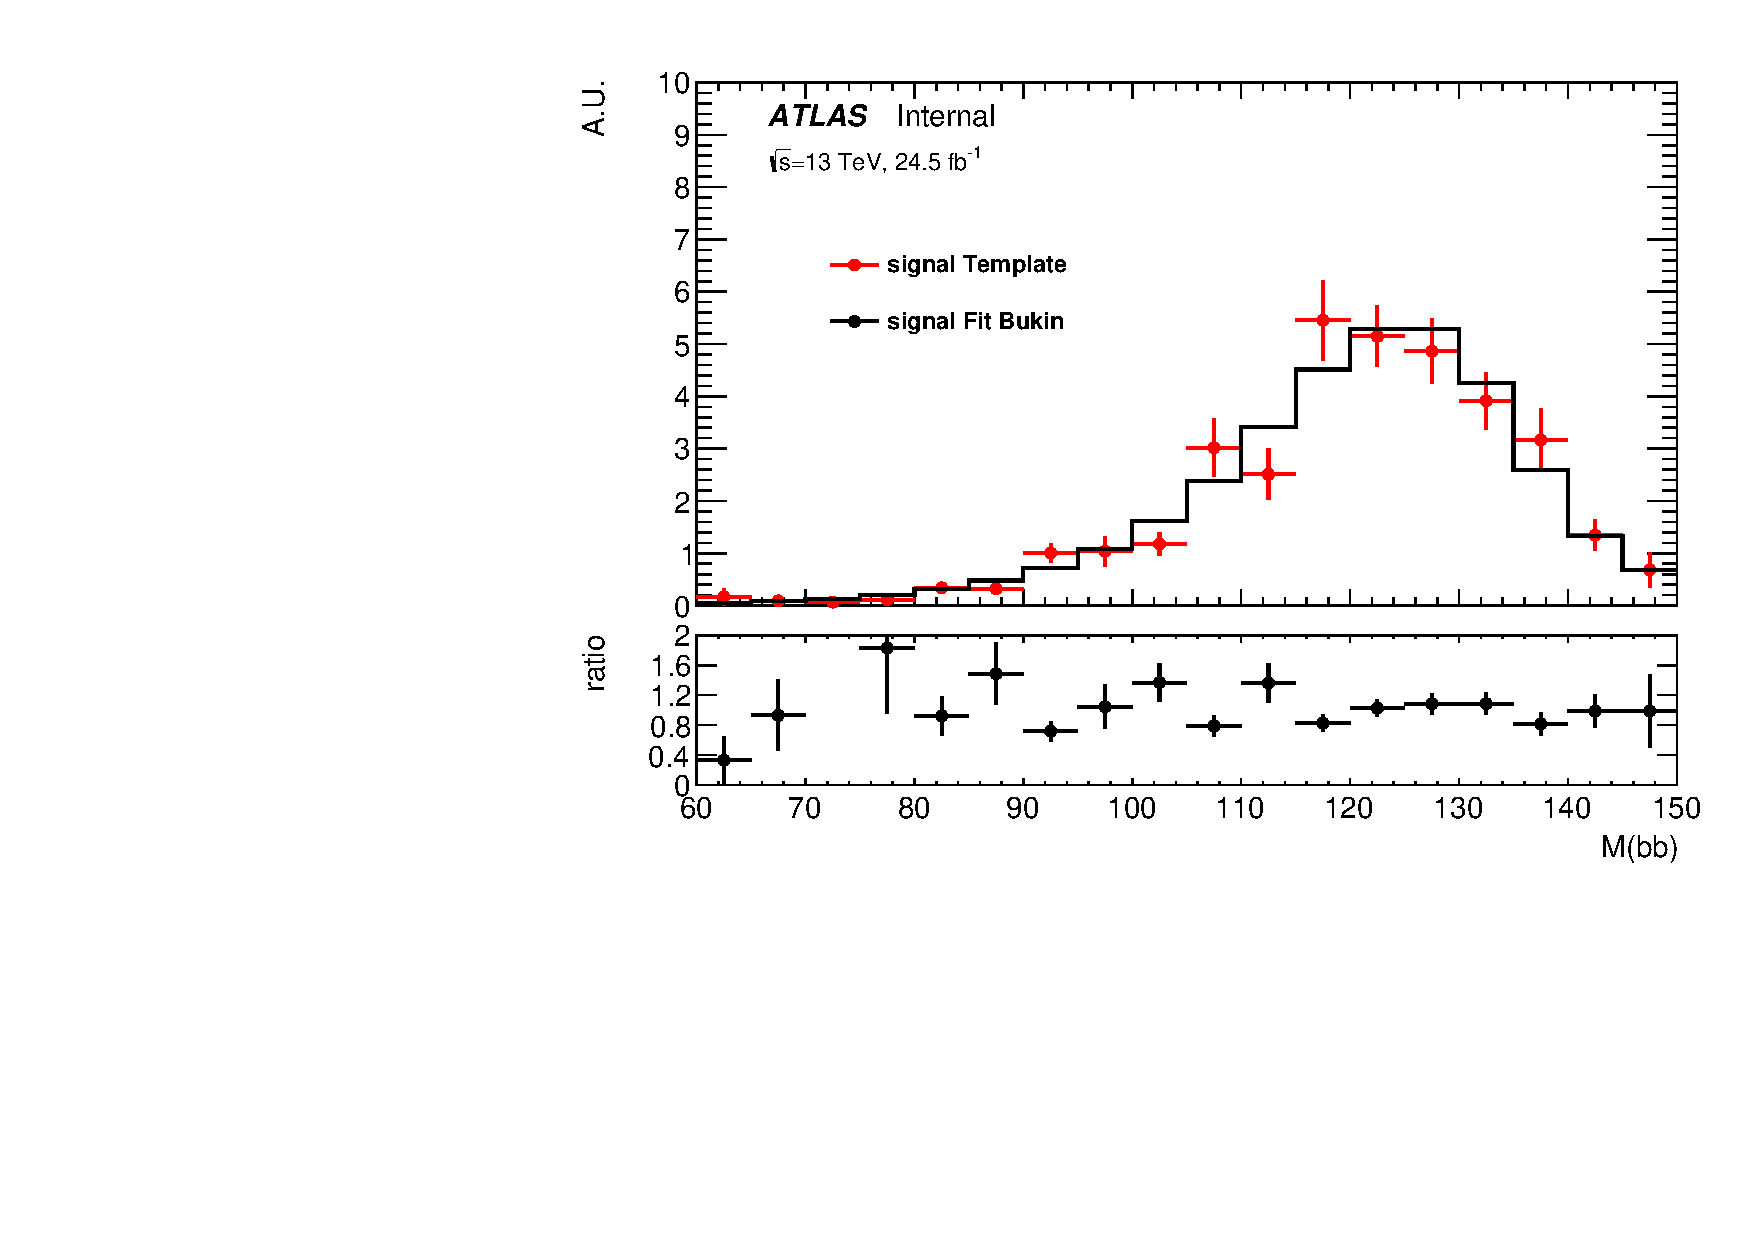
\includegraphics[width=0.24\textwidth]{figures_alt/sig_2cen_SRIII.pdf}
 \includegraphics[width=0.24\textwidth]{figures_alt/sig_2cen_SRIIV.pdf}\\
 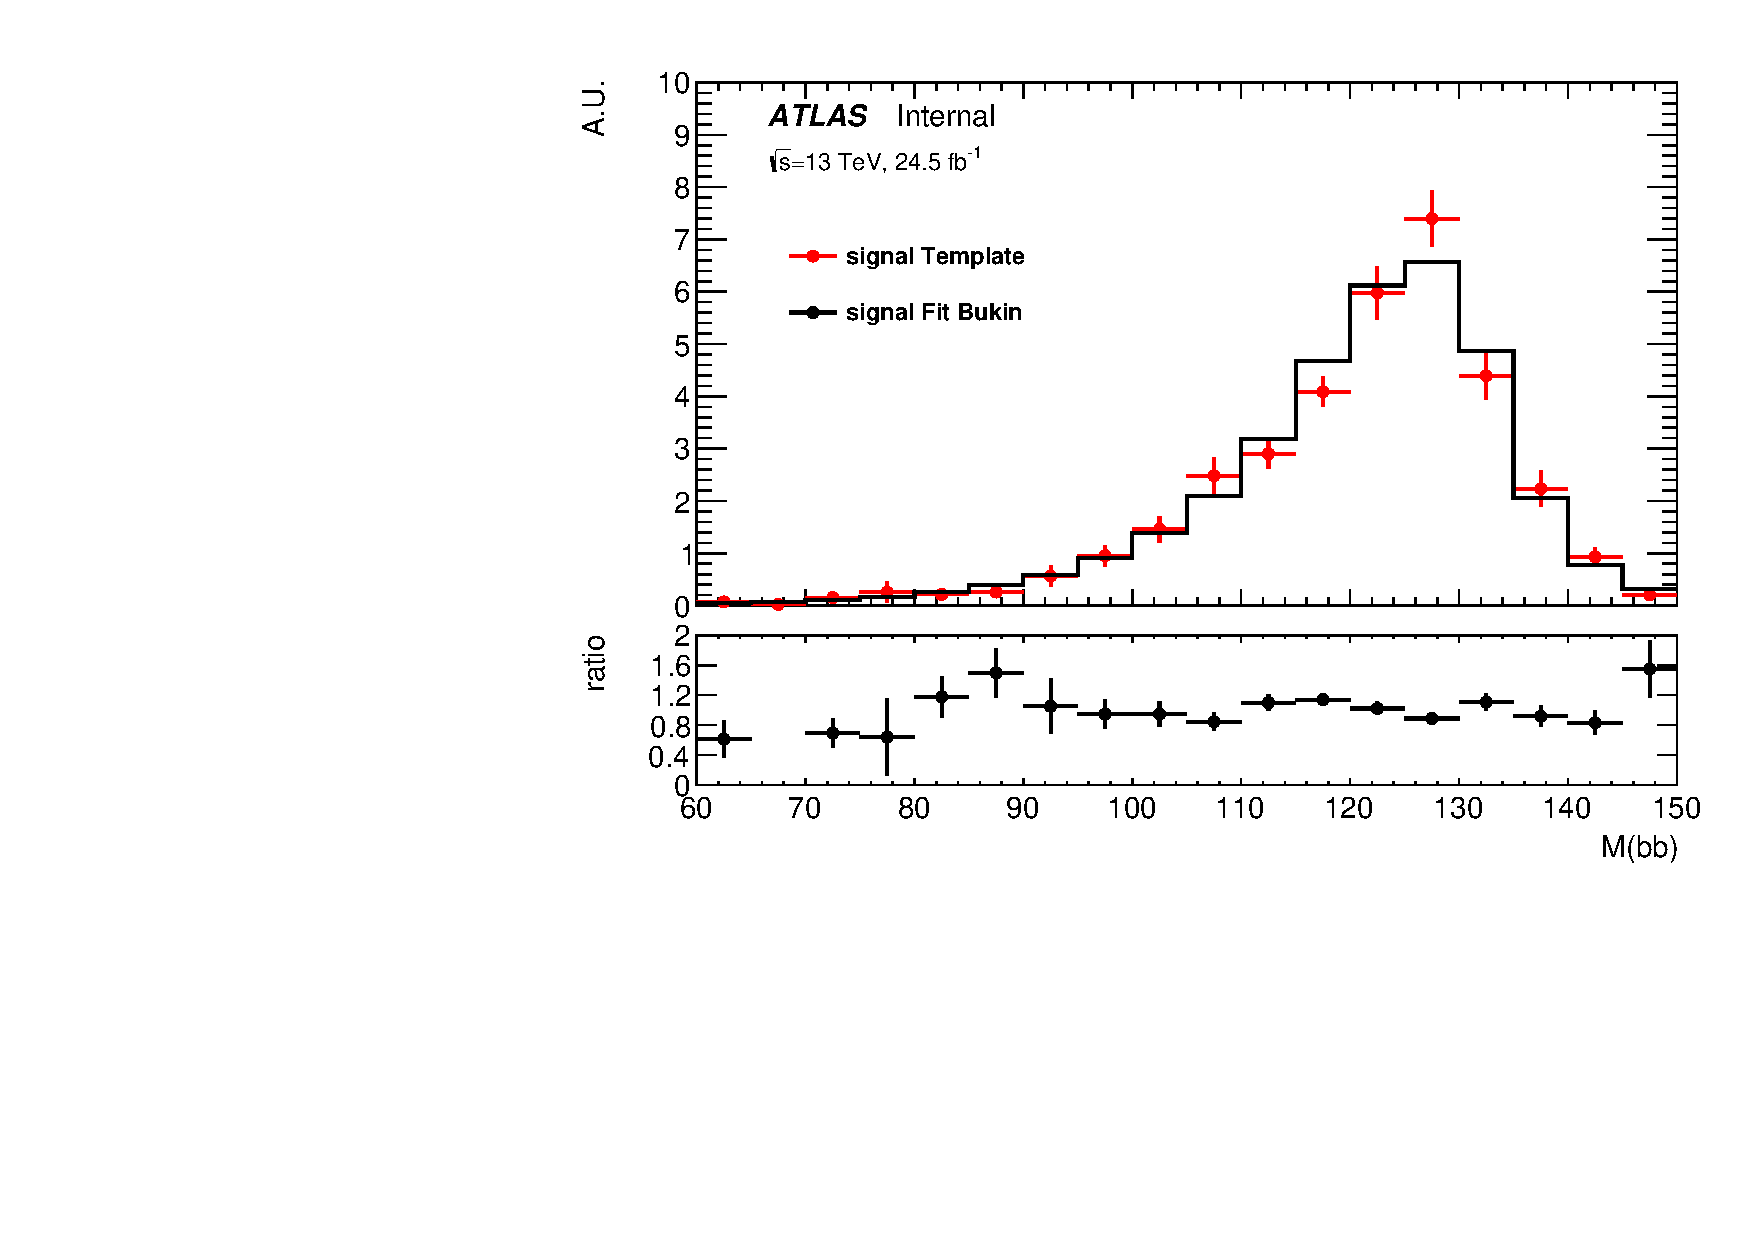
\includegraphics[width=0.24\textwidth]{figures_alt/sig_4cen_SRI.pdf}
 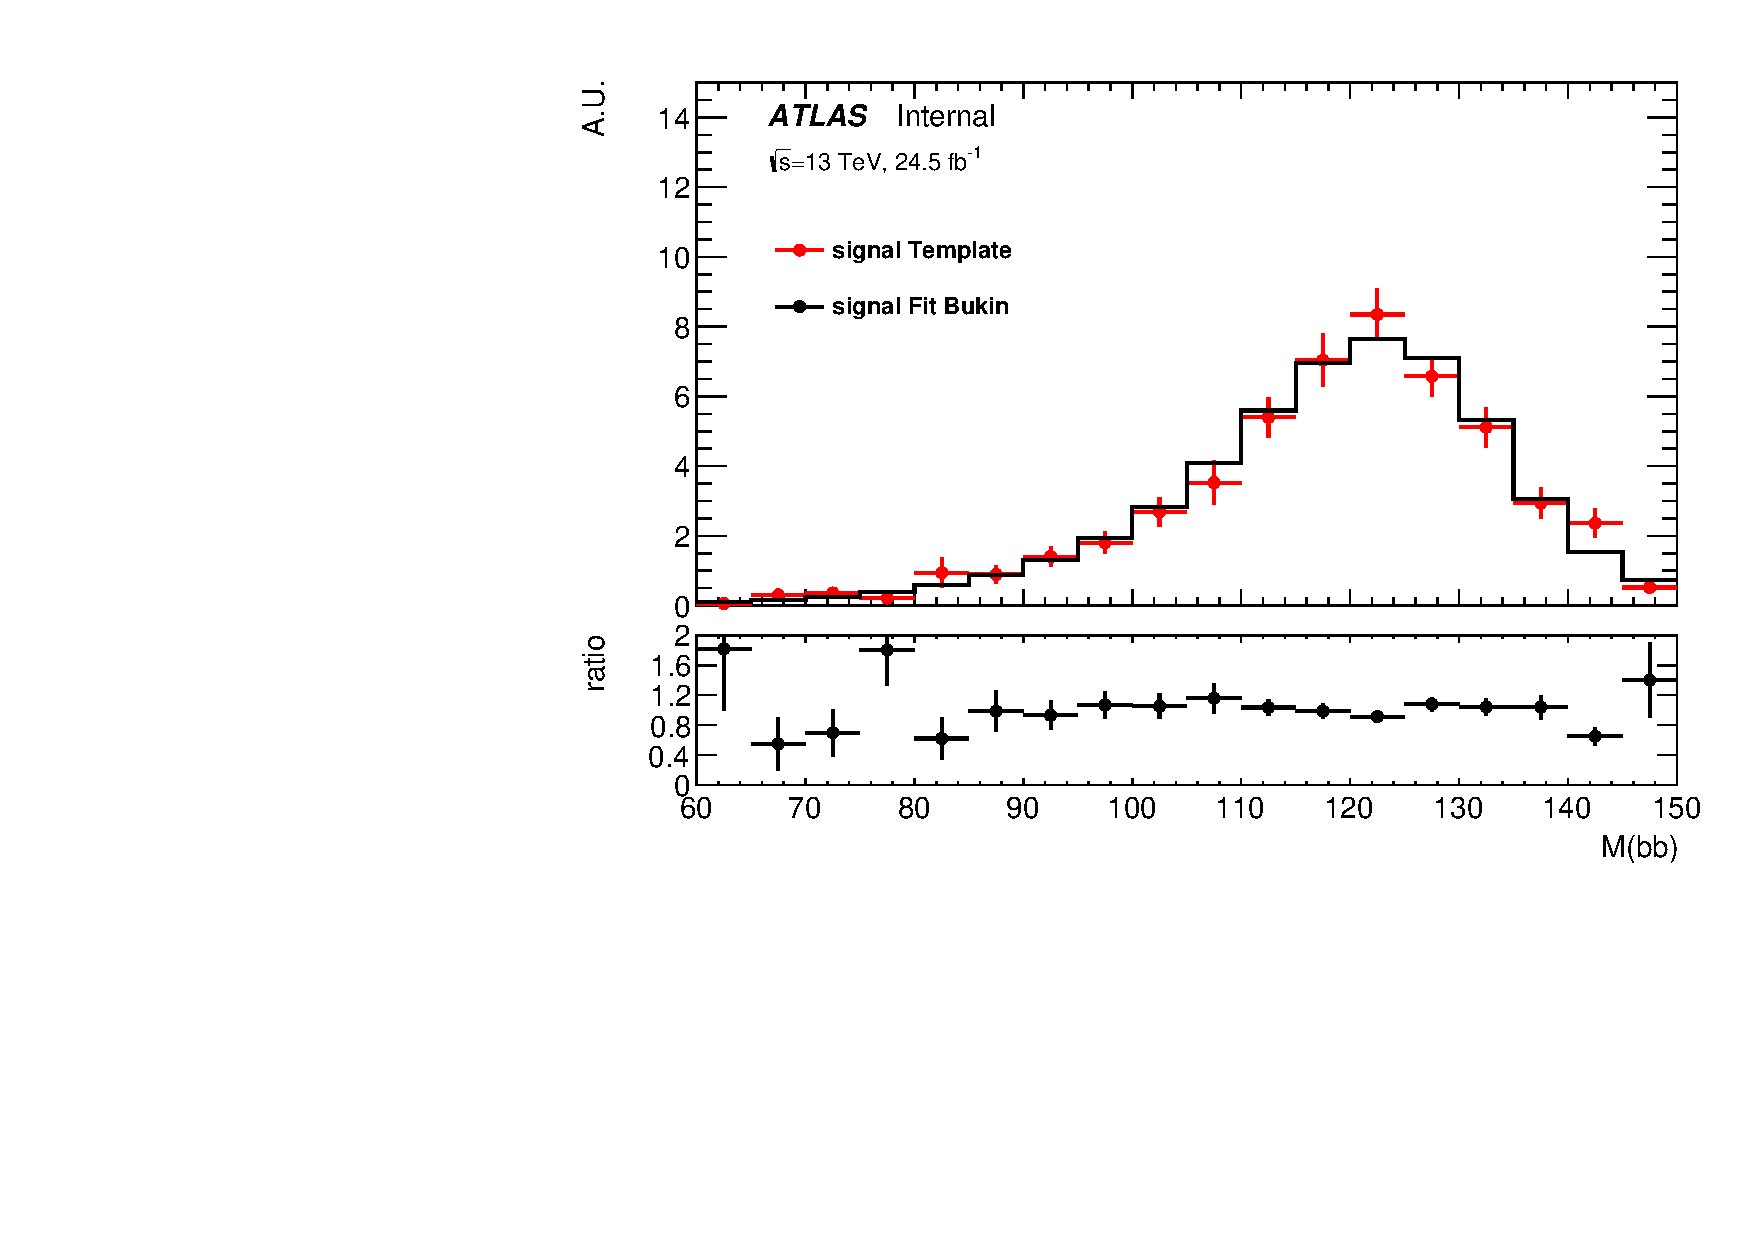
\includegraphics[width=0.24\textwidth]{figures_alt/sig_4cen_SRII.pdf}
 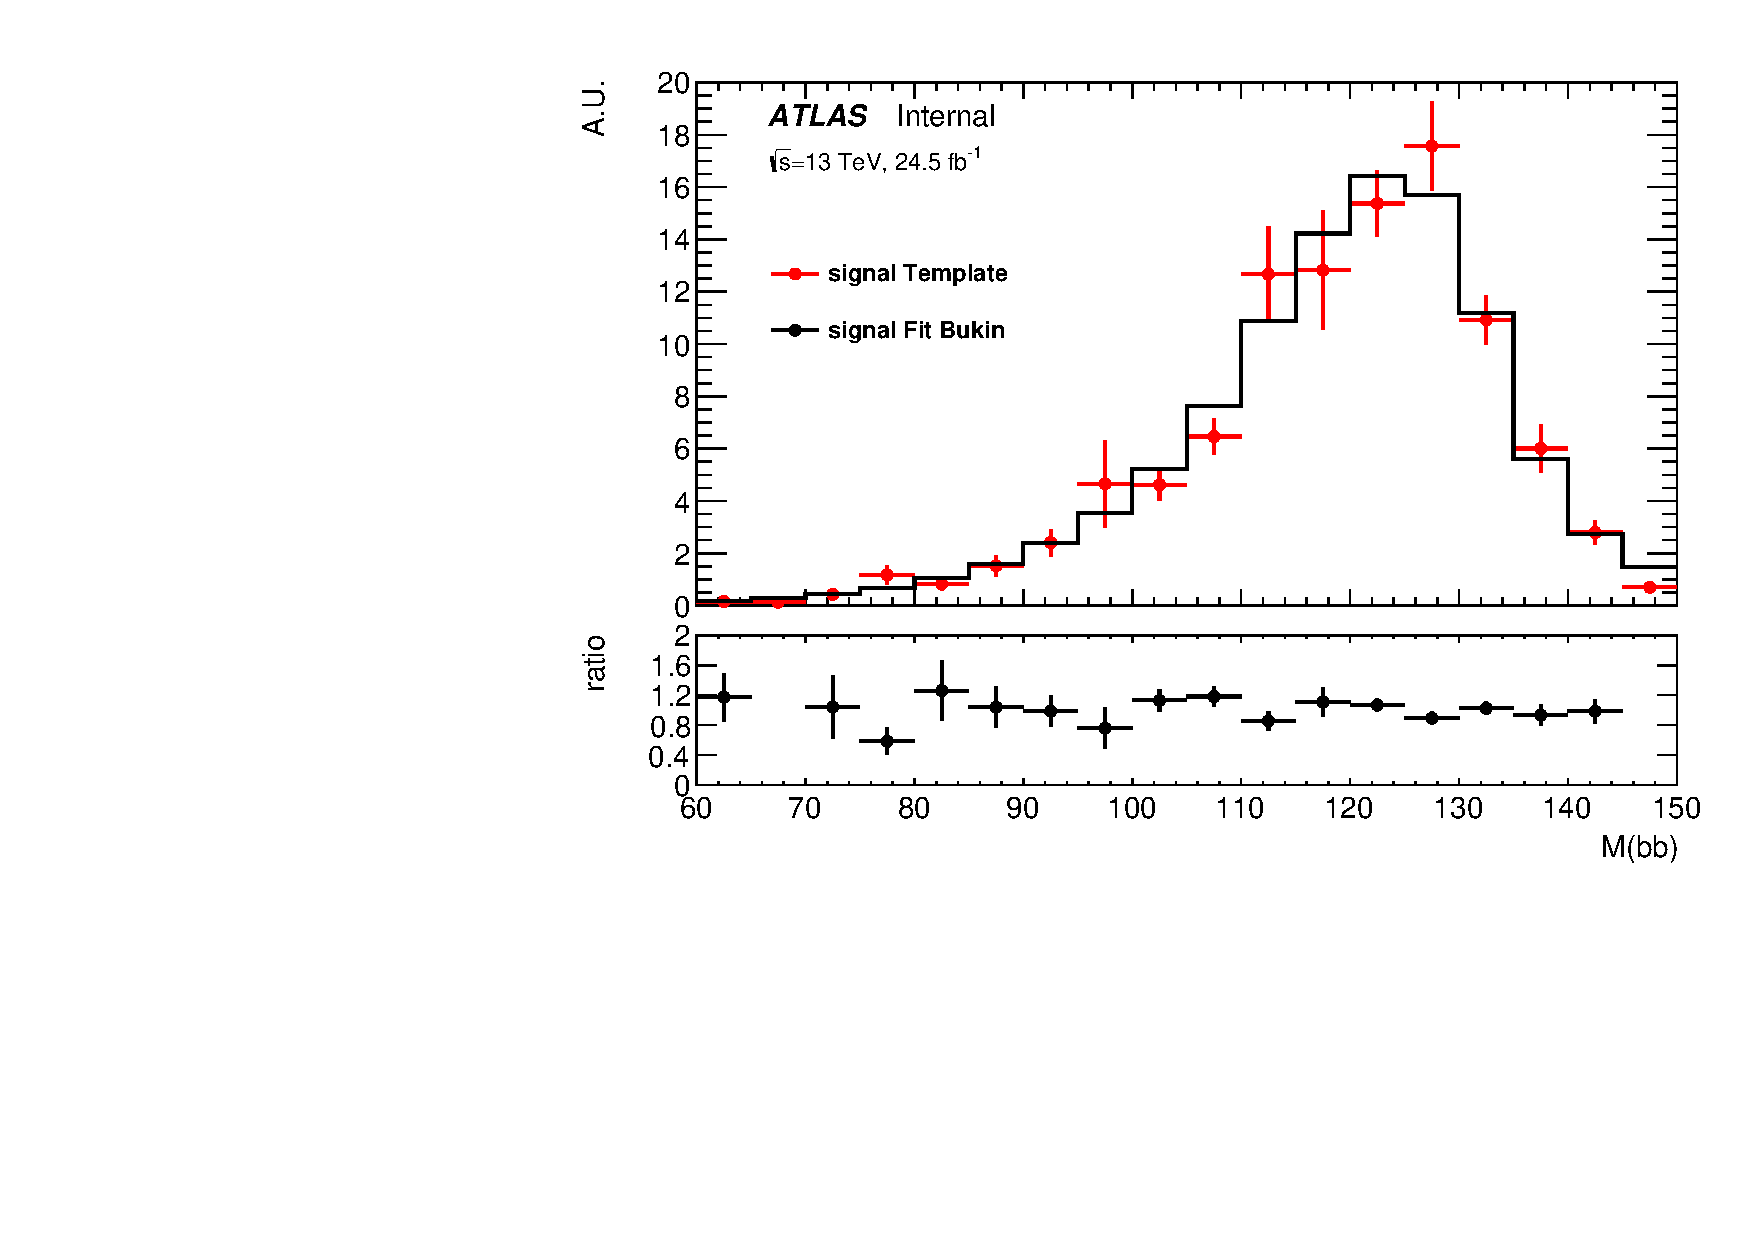
\includegraphics[width=0.24\textwidth]{figures_alt/sig_4cen_SRIII.pdf}
 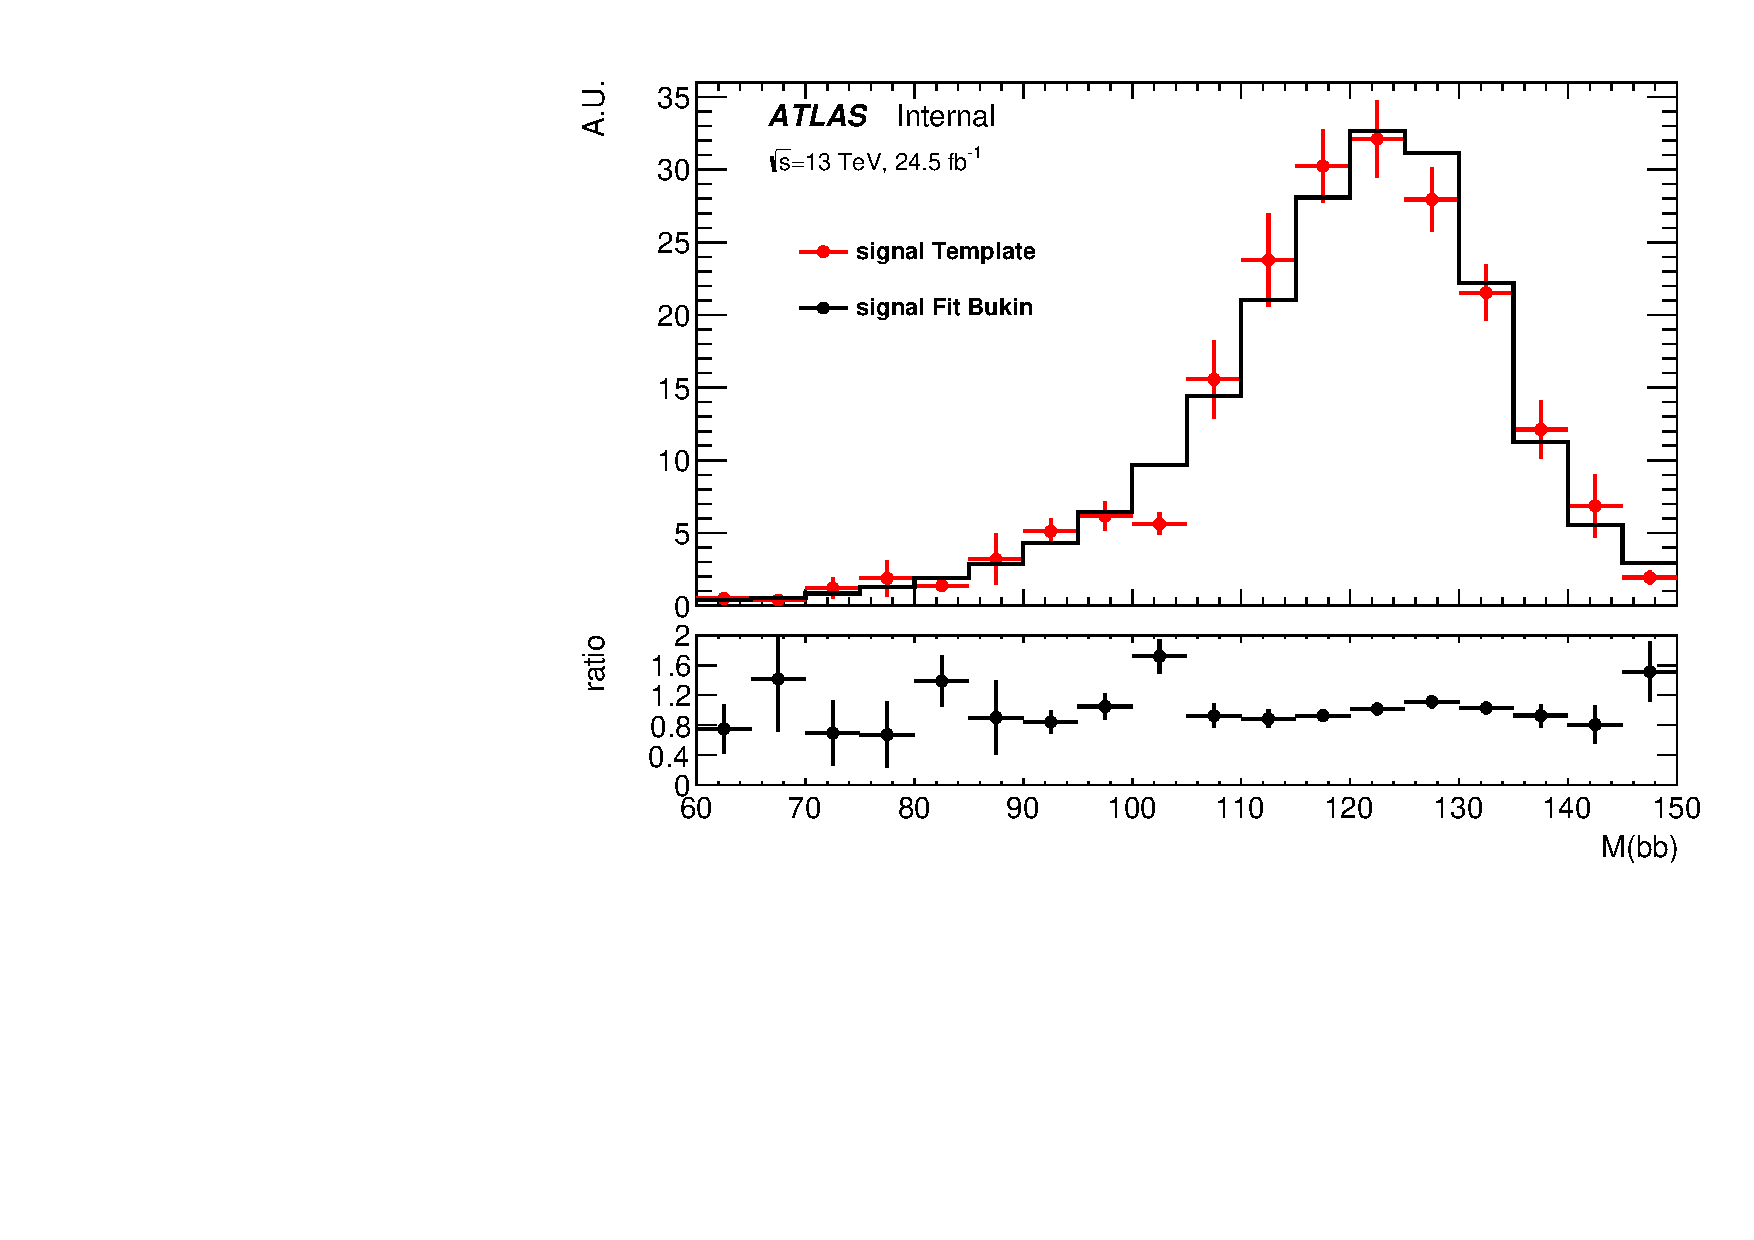
\includegraphics[width=0.24\textwidth]{figures_alt/sig_4cen_SRIV.pdf}

\caption{Bukin function parametrization of signal \Mbb{} distributions of SR I to SR IV (left to right) in \twocentral (top) and \fourcentral (bottom) channels}
  \label{fig:sigpar_alt}
\end{figure}


\begin{figure}[htbp]
  \centering    
 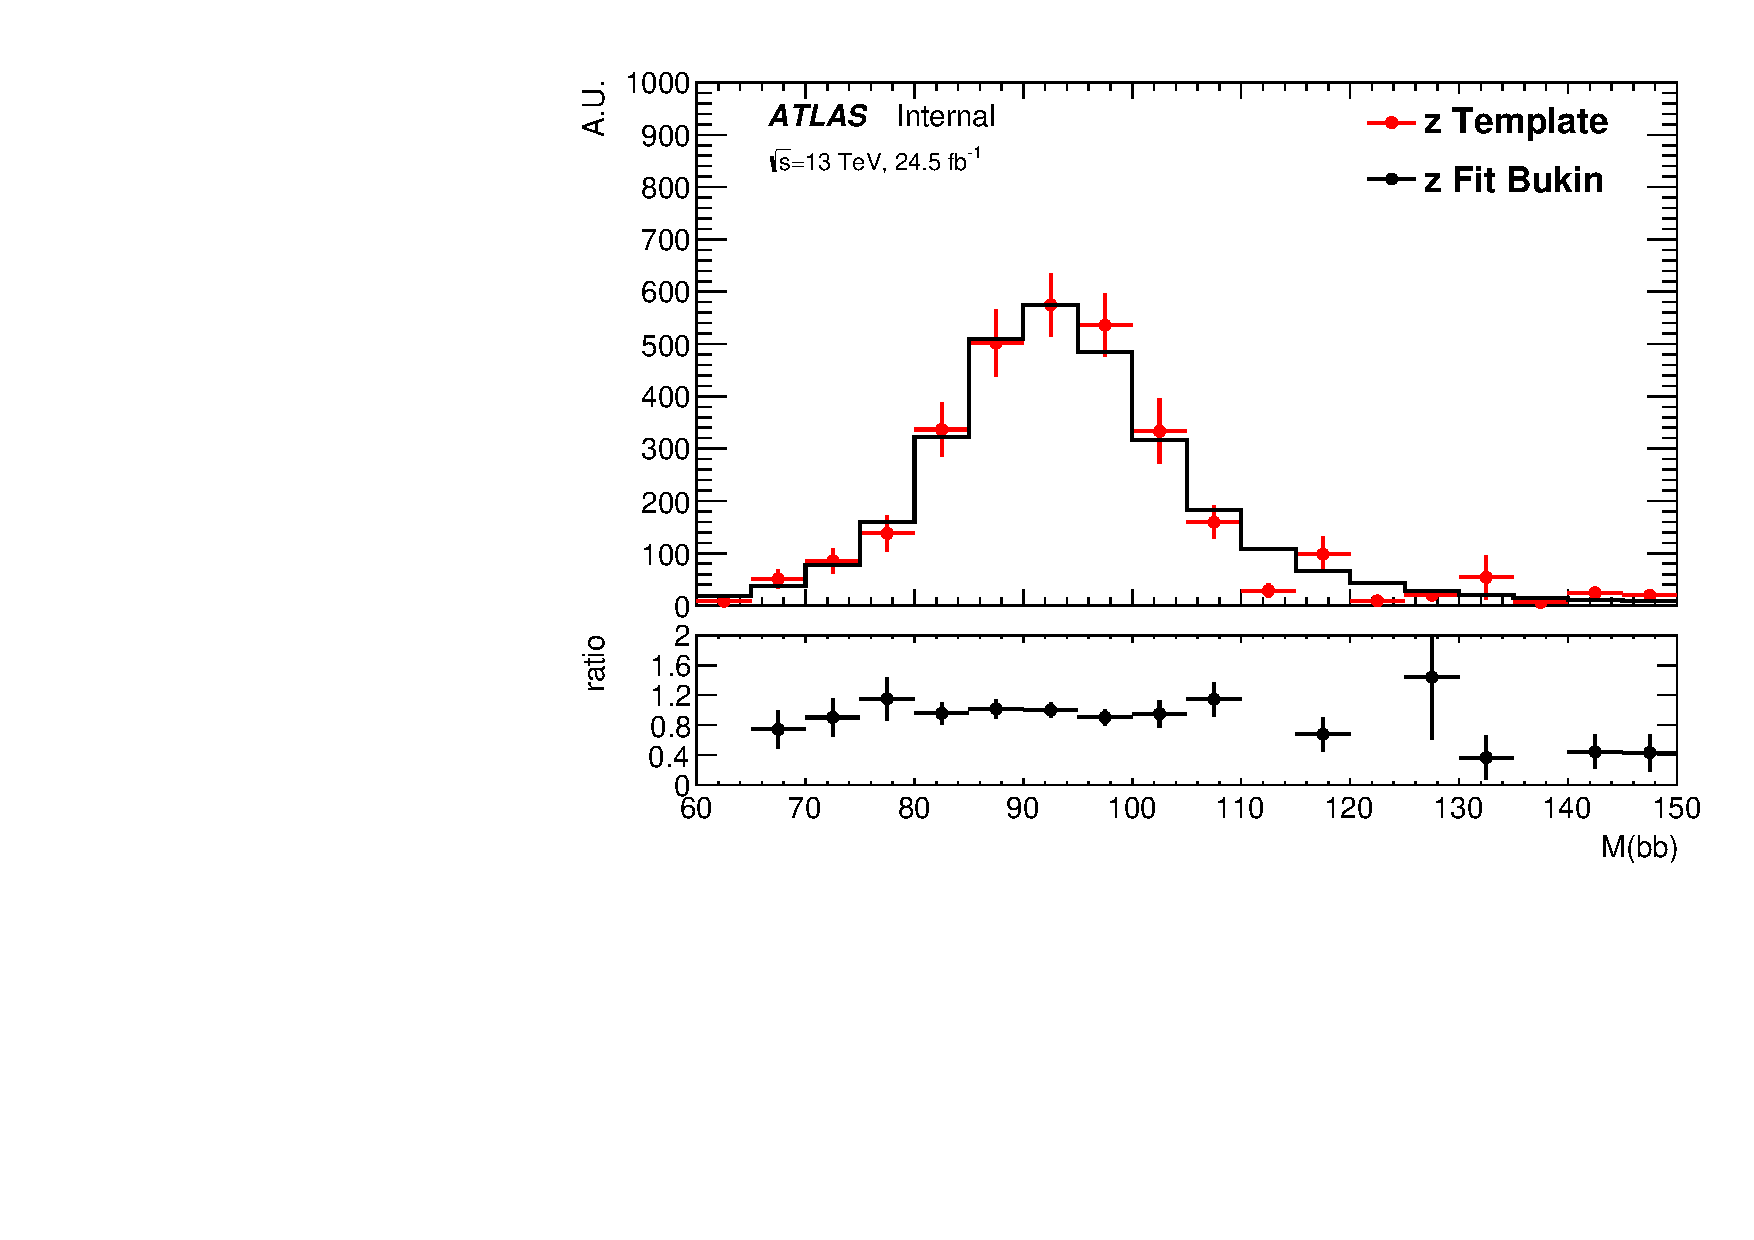
\includegraphics[width=0.45\textwidth]{figures/SigPar/z_2cen.pdf}
 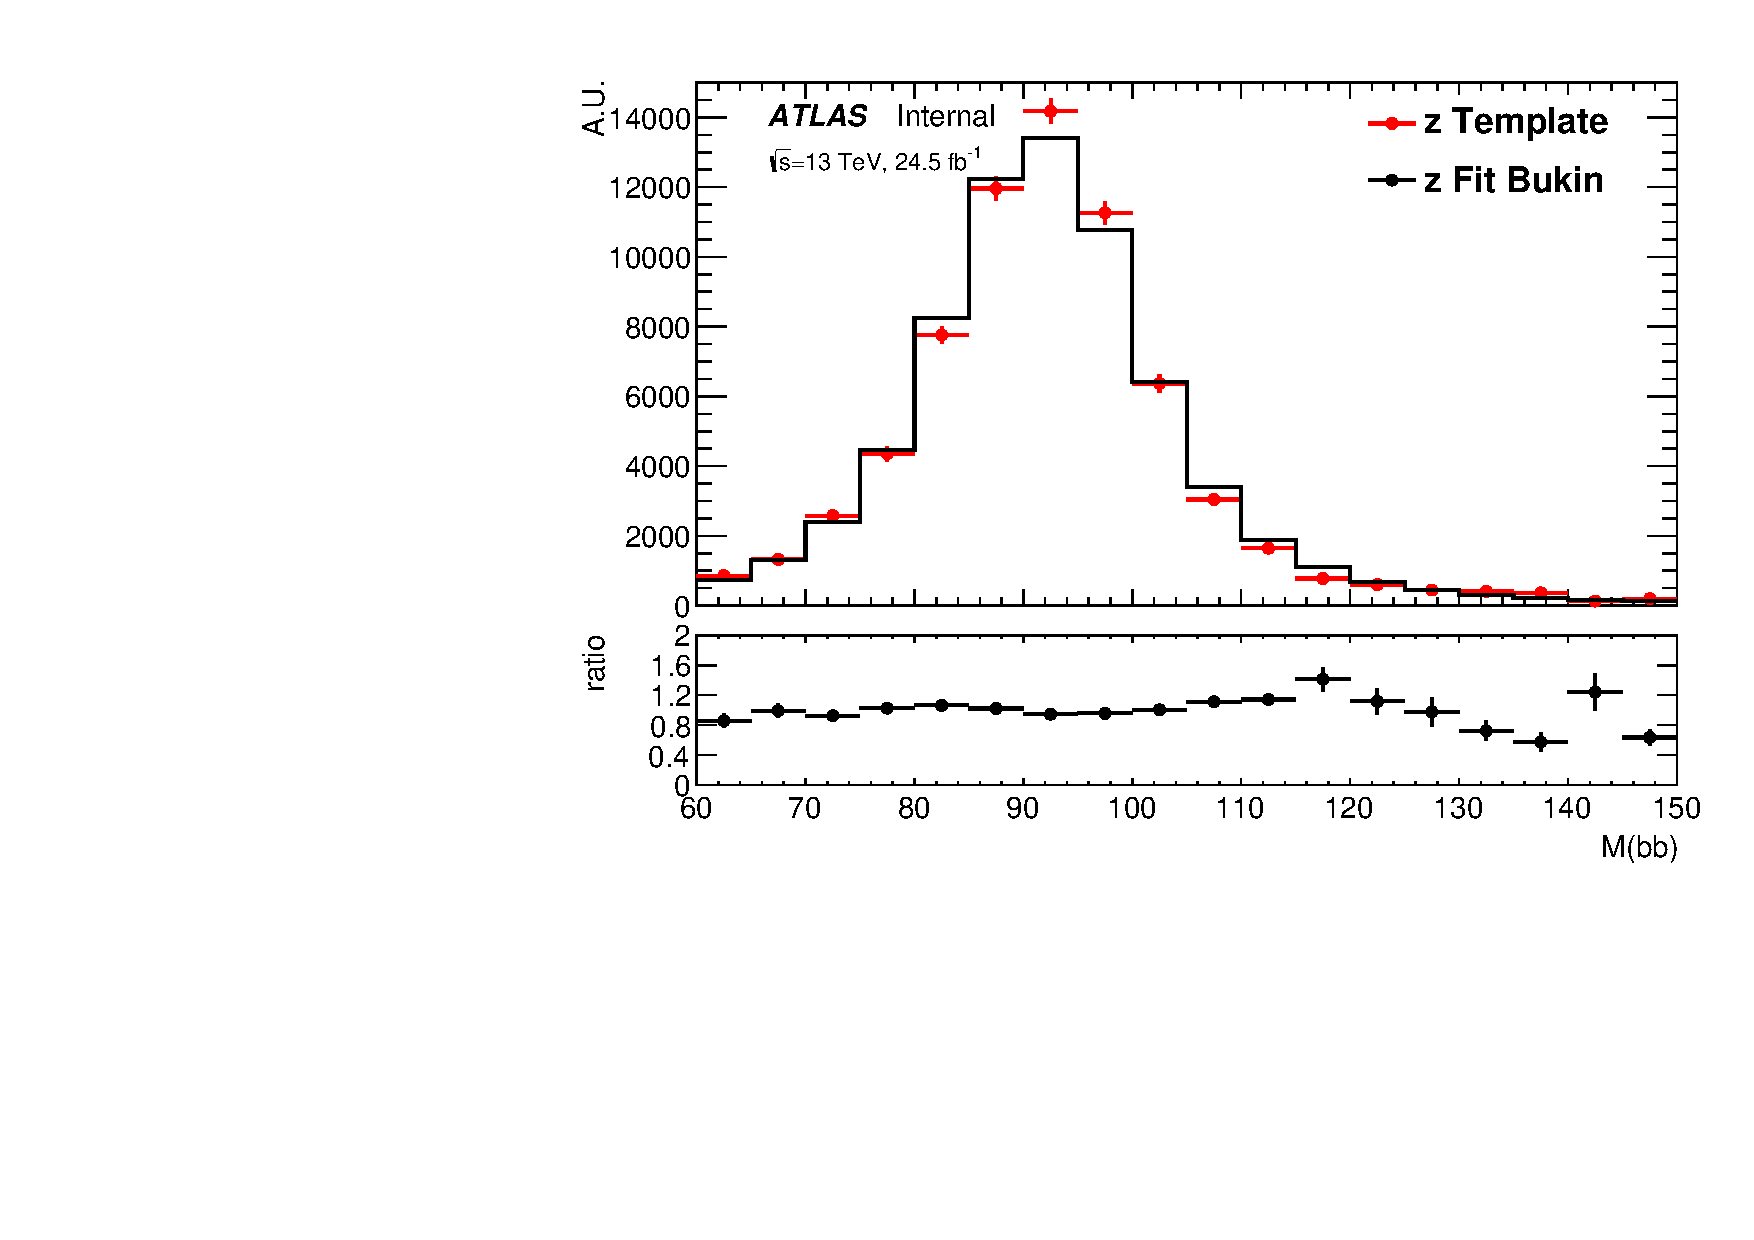
\includegraphics[width=0.45\textwidth]{figures/SigPar/z_4cen.pdf}

\caption{Bukin function parametrization of \zjets~\Mbb{} distribution in \twocentral (left) and \fourcentral (right)}
\label{fig:zpar_alt}
\end{figure}

\begin{table}[]
\centering
\caption{Goodness of fit for the Bukin parametertizationns and signal and \zjets{} \Mbb{} distributions.}
\label{tab:sigpar}
\begin{tabular}{|l|l|l|l|l|}
\hline
Process                  & Signal \twocentral SR I  & Signal \twocentral SR II  & Signal \twocentral SR III  & Signal \twocentral SR IV  \\ \hline
$\chi^2$ ($\chi^2$ Prob) & 1.27 (0.21)              & 0.73 (0.71)               & 0.87 (0.60)                & 1.02 (0.43)               \\ \hline
Process                  & Signal \fourcentral SR I & Signal \fourcentral SR II & Signal \fourcentral SR III & Signal \fourcentral SR IV \\ \hline
$\chi^2$ ($\chi^2$ Prob) & 1.06 (0.39)              & 0.77 (0.71)               & 1.10 (0.35)                & 1.21 (0.25)               \\ \hline
Process                  & \zjets \twocentral       & \zjets \fourcentral       &                            &                           \\ \hline
$\chi^2$ ($\chi^2$ Prob) & 1.7 (0.04)               & 1.32 (0.17)               &                            &                           \\ \hline
\end{tabular}
\end{table}% 



\subsubsection{Non-resonant \Mbb{} distribution}
\label{sec:nonres_alt}

Given that a potentially large bias could be induced by the assumption that all regions BDT regions 
have the same shape modulo a difference that could be explained by a linear transfer function, we fit each 
of the BDT region backgrounds independently with an analytical function. The sidebands of the \Mbb{} 
distribution of each BDT region are shown in Fig. \ref{fig:mbb_sidebands}.

\begin{figure}[htbp]
  \centering
 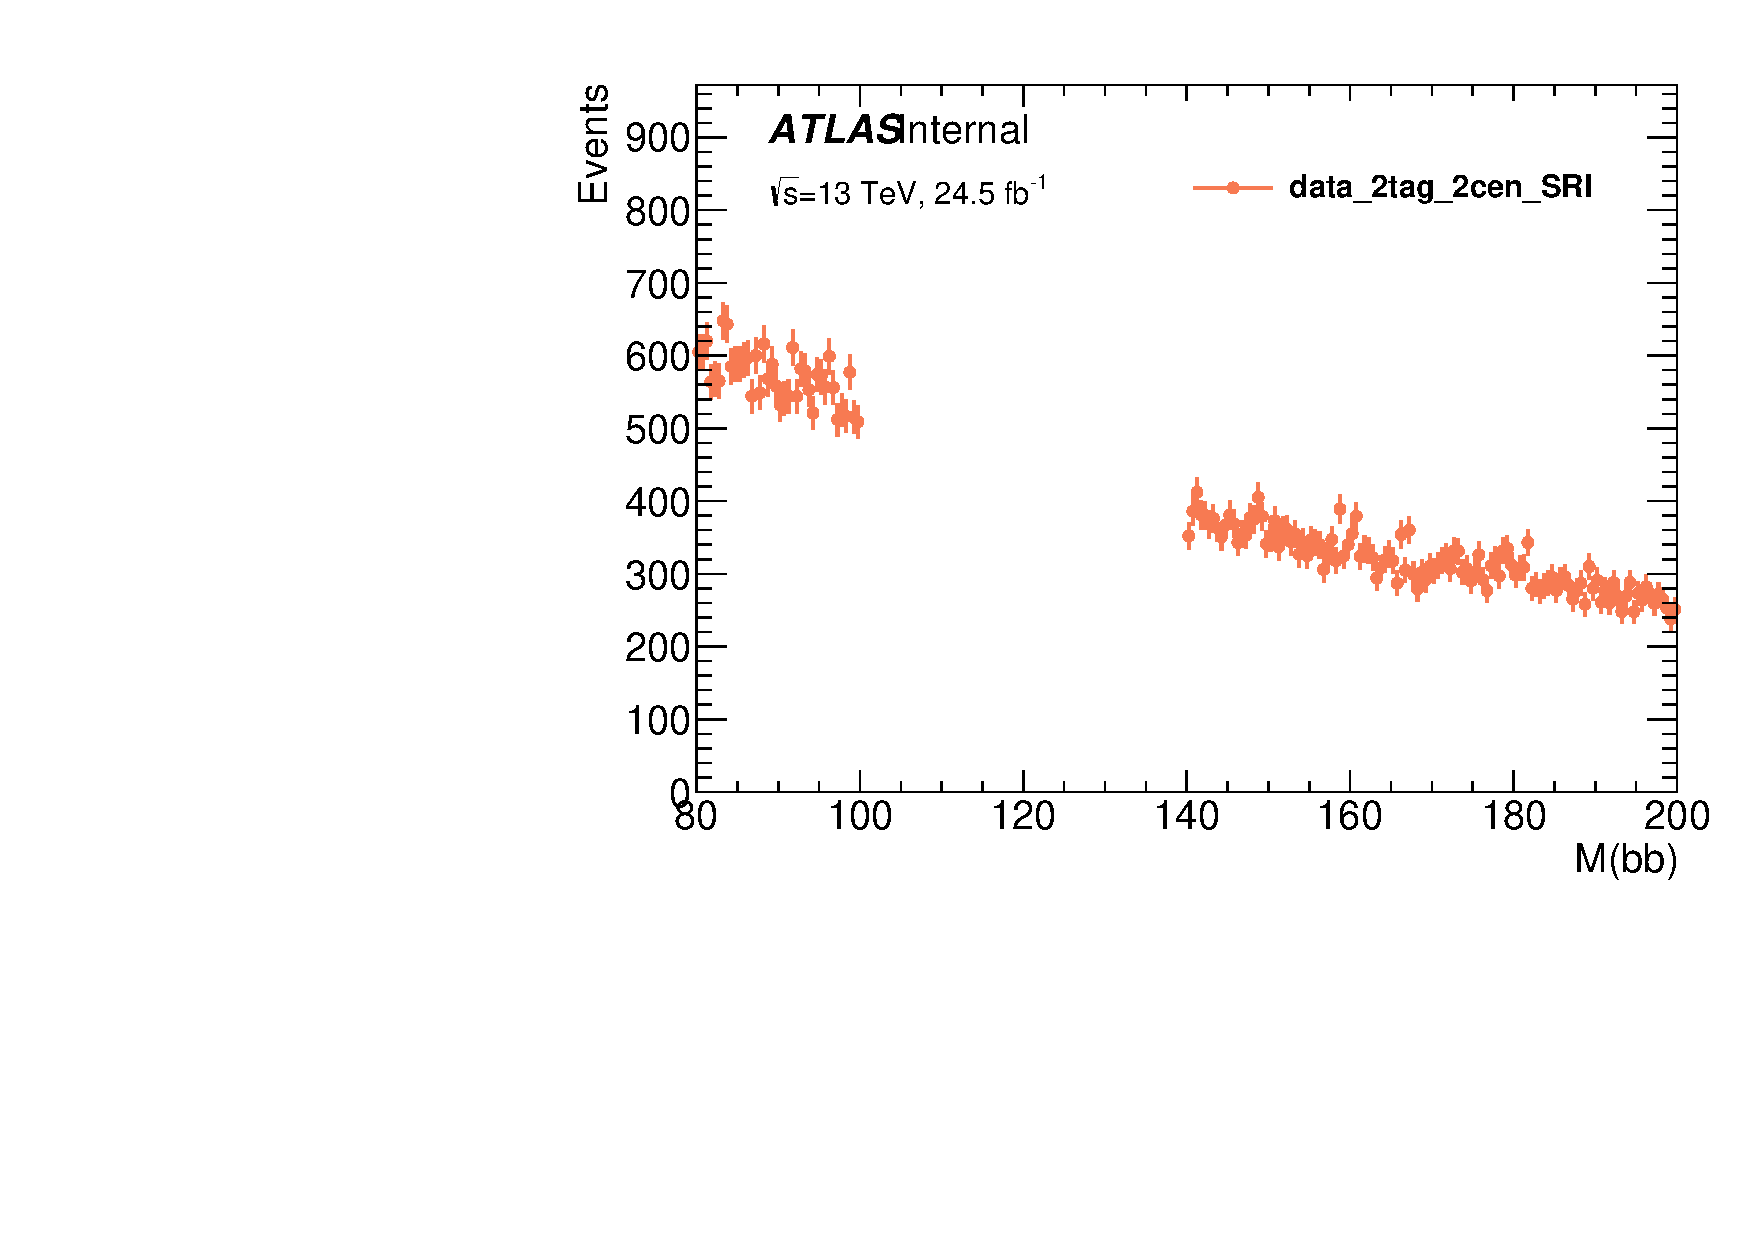
\includegraphics[width=0.45\textwidth]{figures_alt/Mbb_SRI_2cen.pdf}
 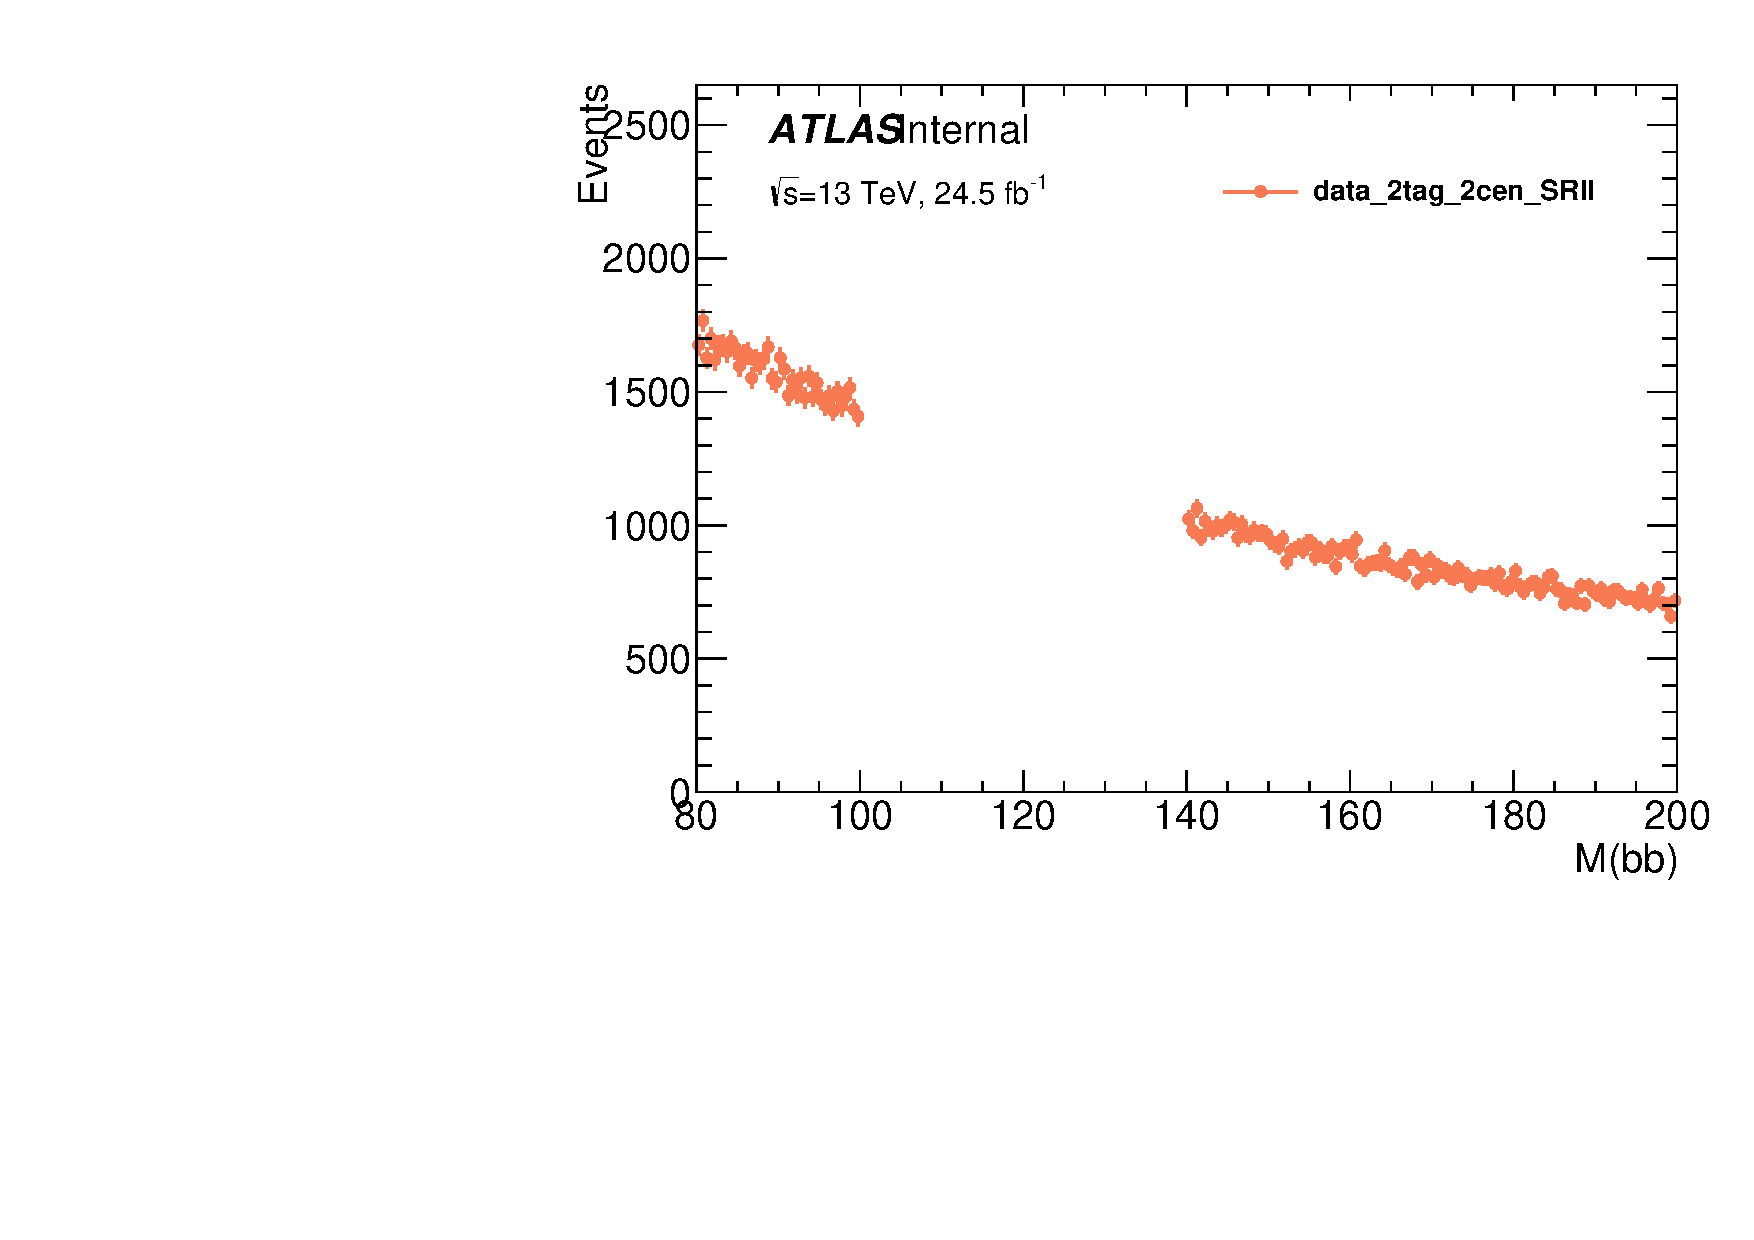
\includegraphics[width=0.45\textwidth]{figures_alt/Mbb_SRII_2cen.pdf}\\
 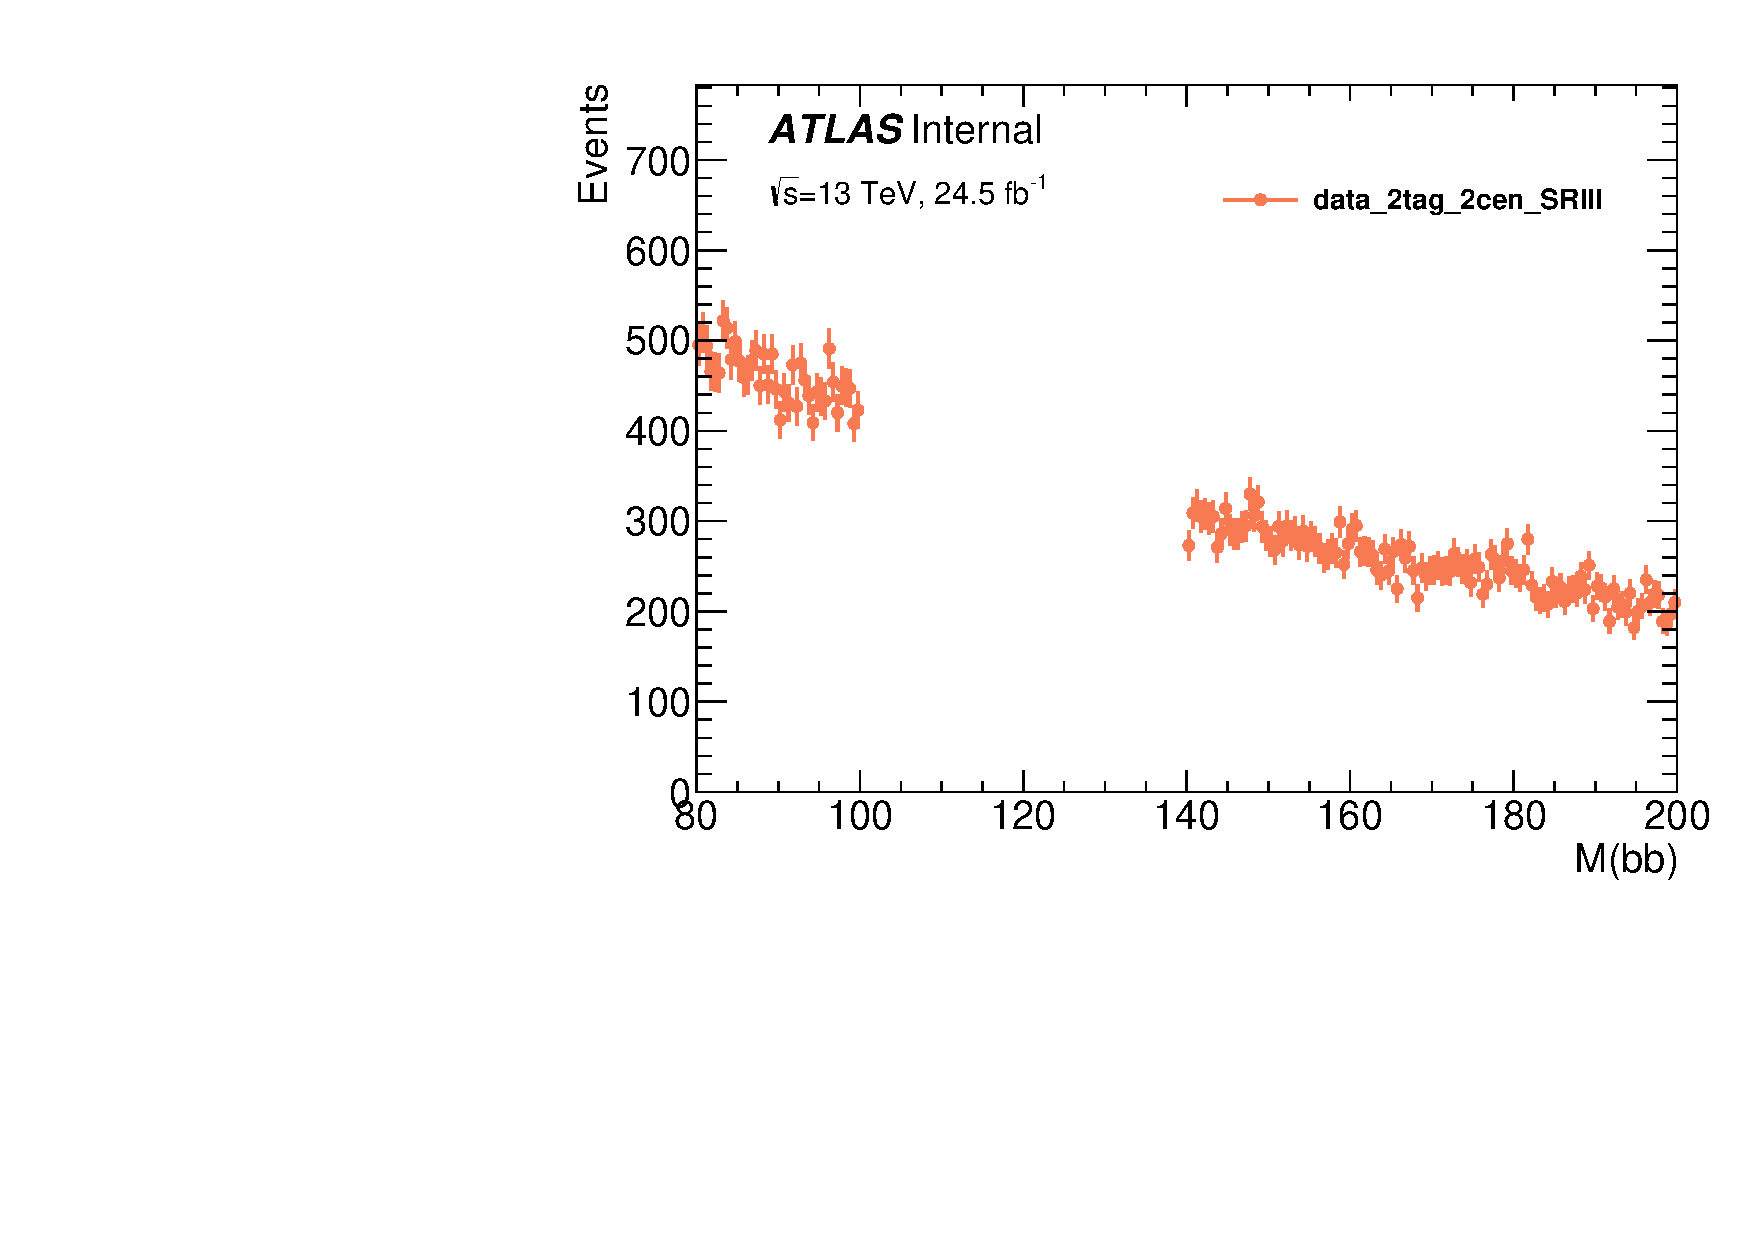
\includegraphics[width=0.45\textwidth]{figures_alt/Mbb_SRIII_2cen.pdf}
 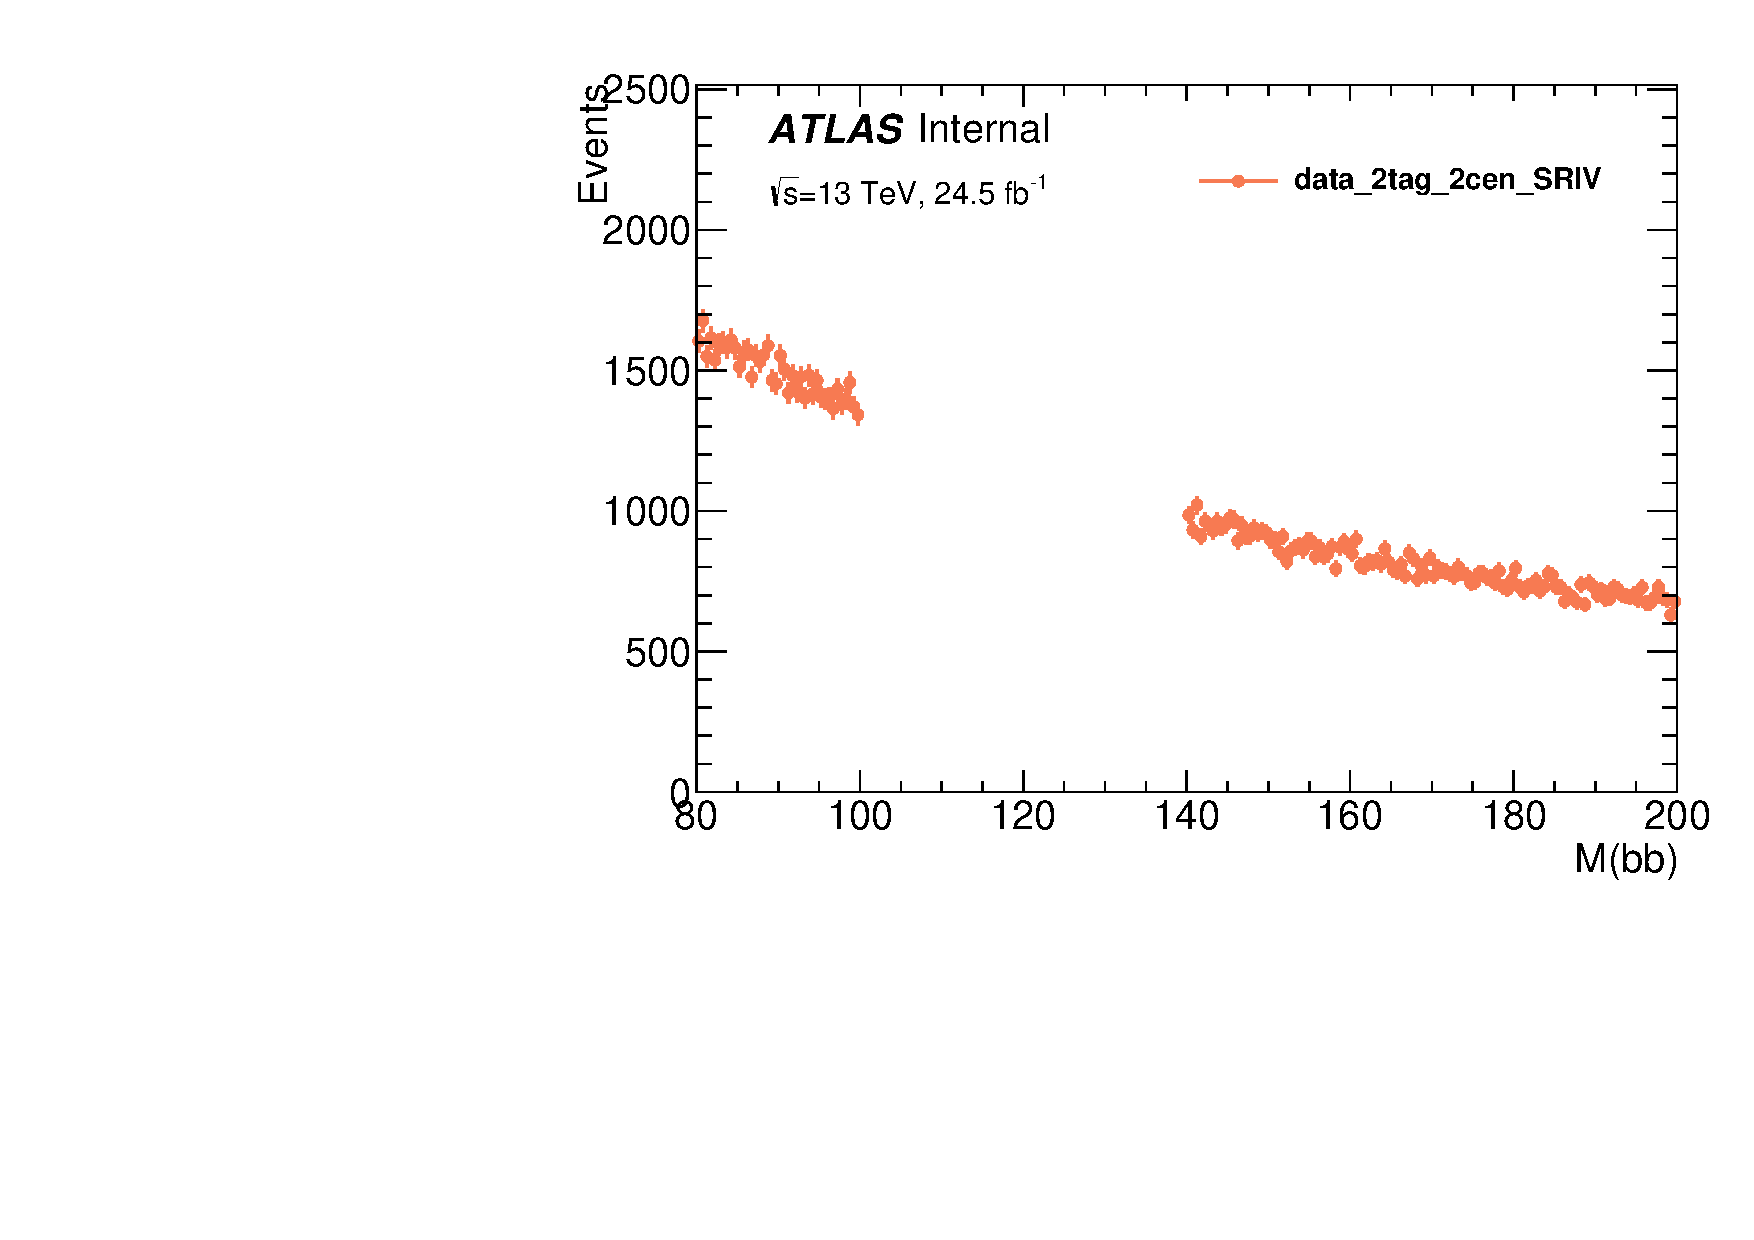
\includegraphics[width=0.45\textwidth]{figures_alt/Mbb_SRIV_2cen.pdf}\\
 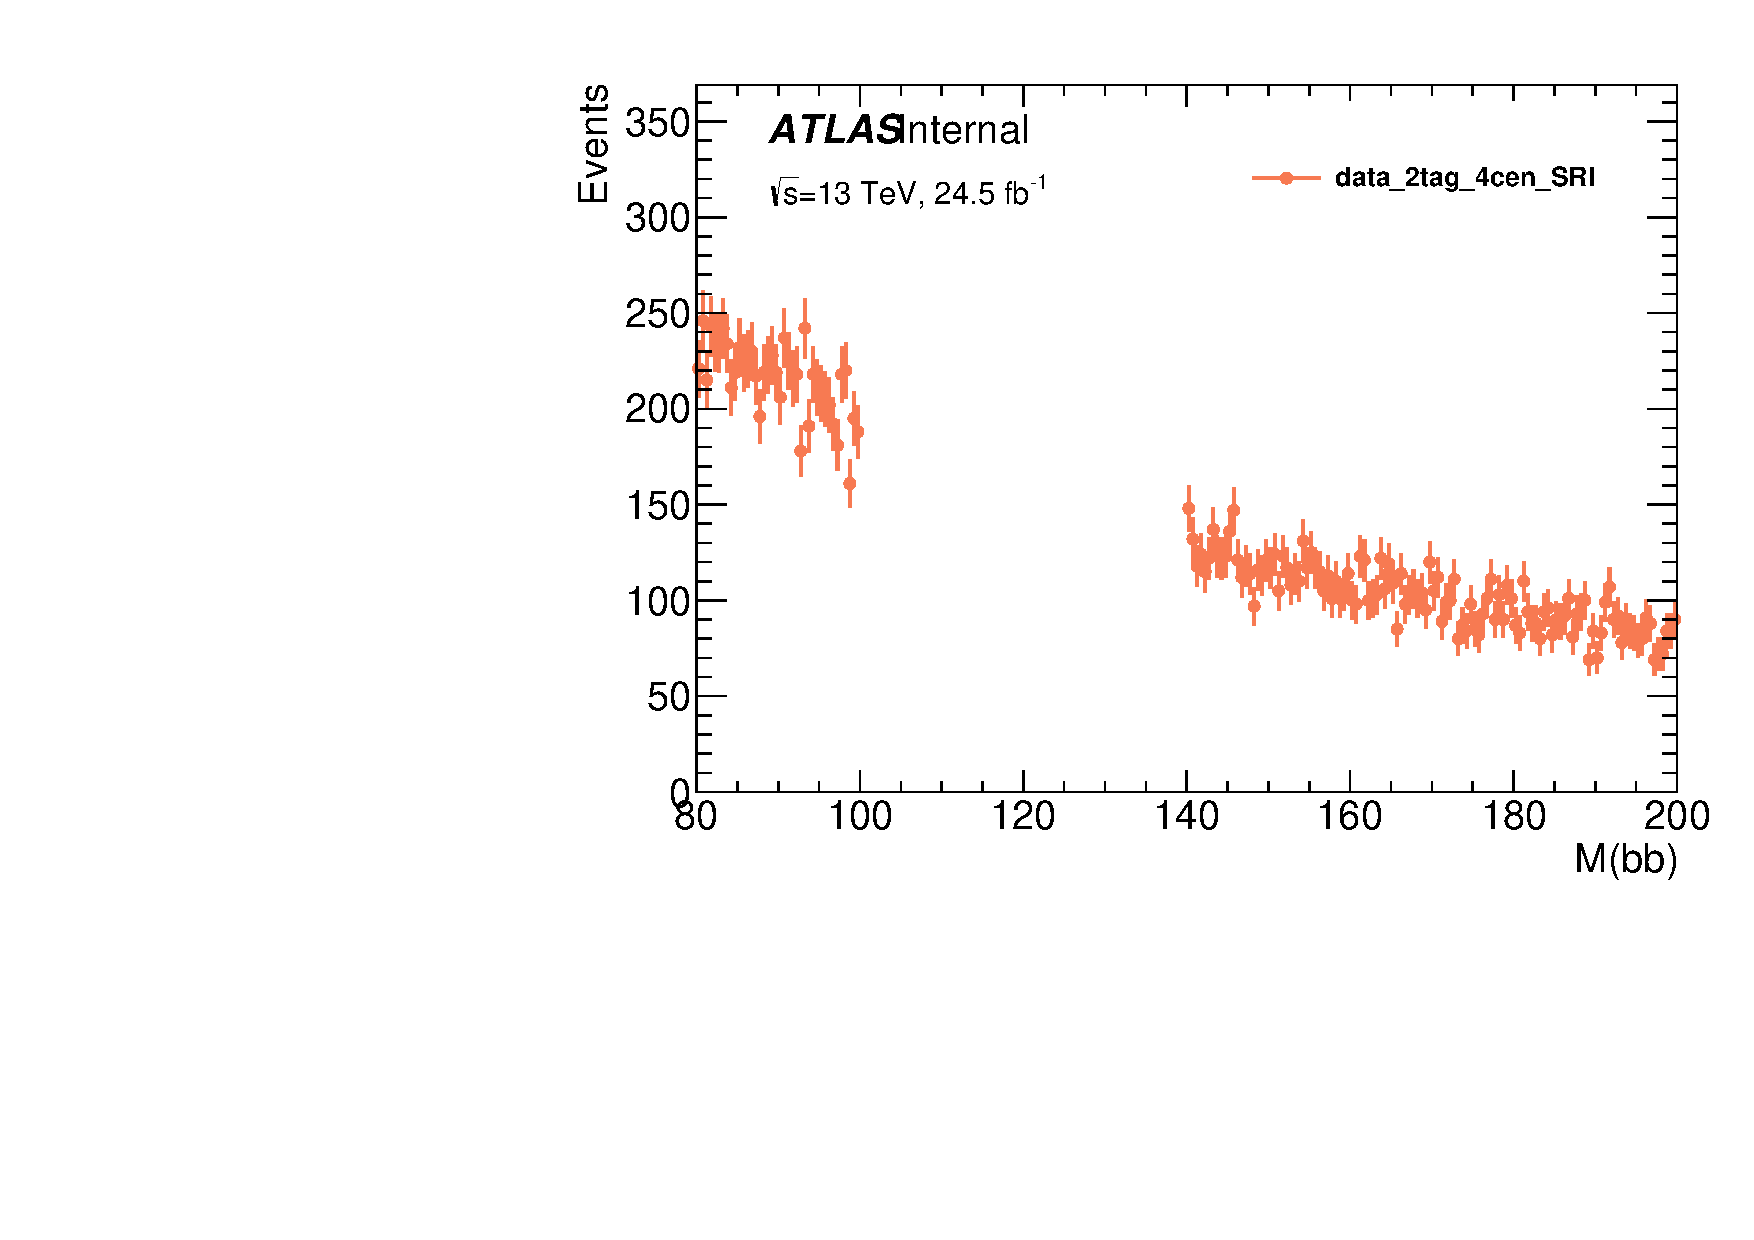
\includegraphics[width=0.45\textwidth]{figures_alt/Mbb_SRI_4cen.pdf}
 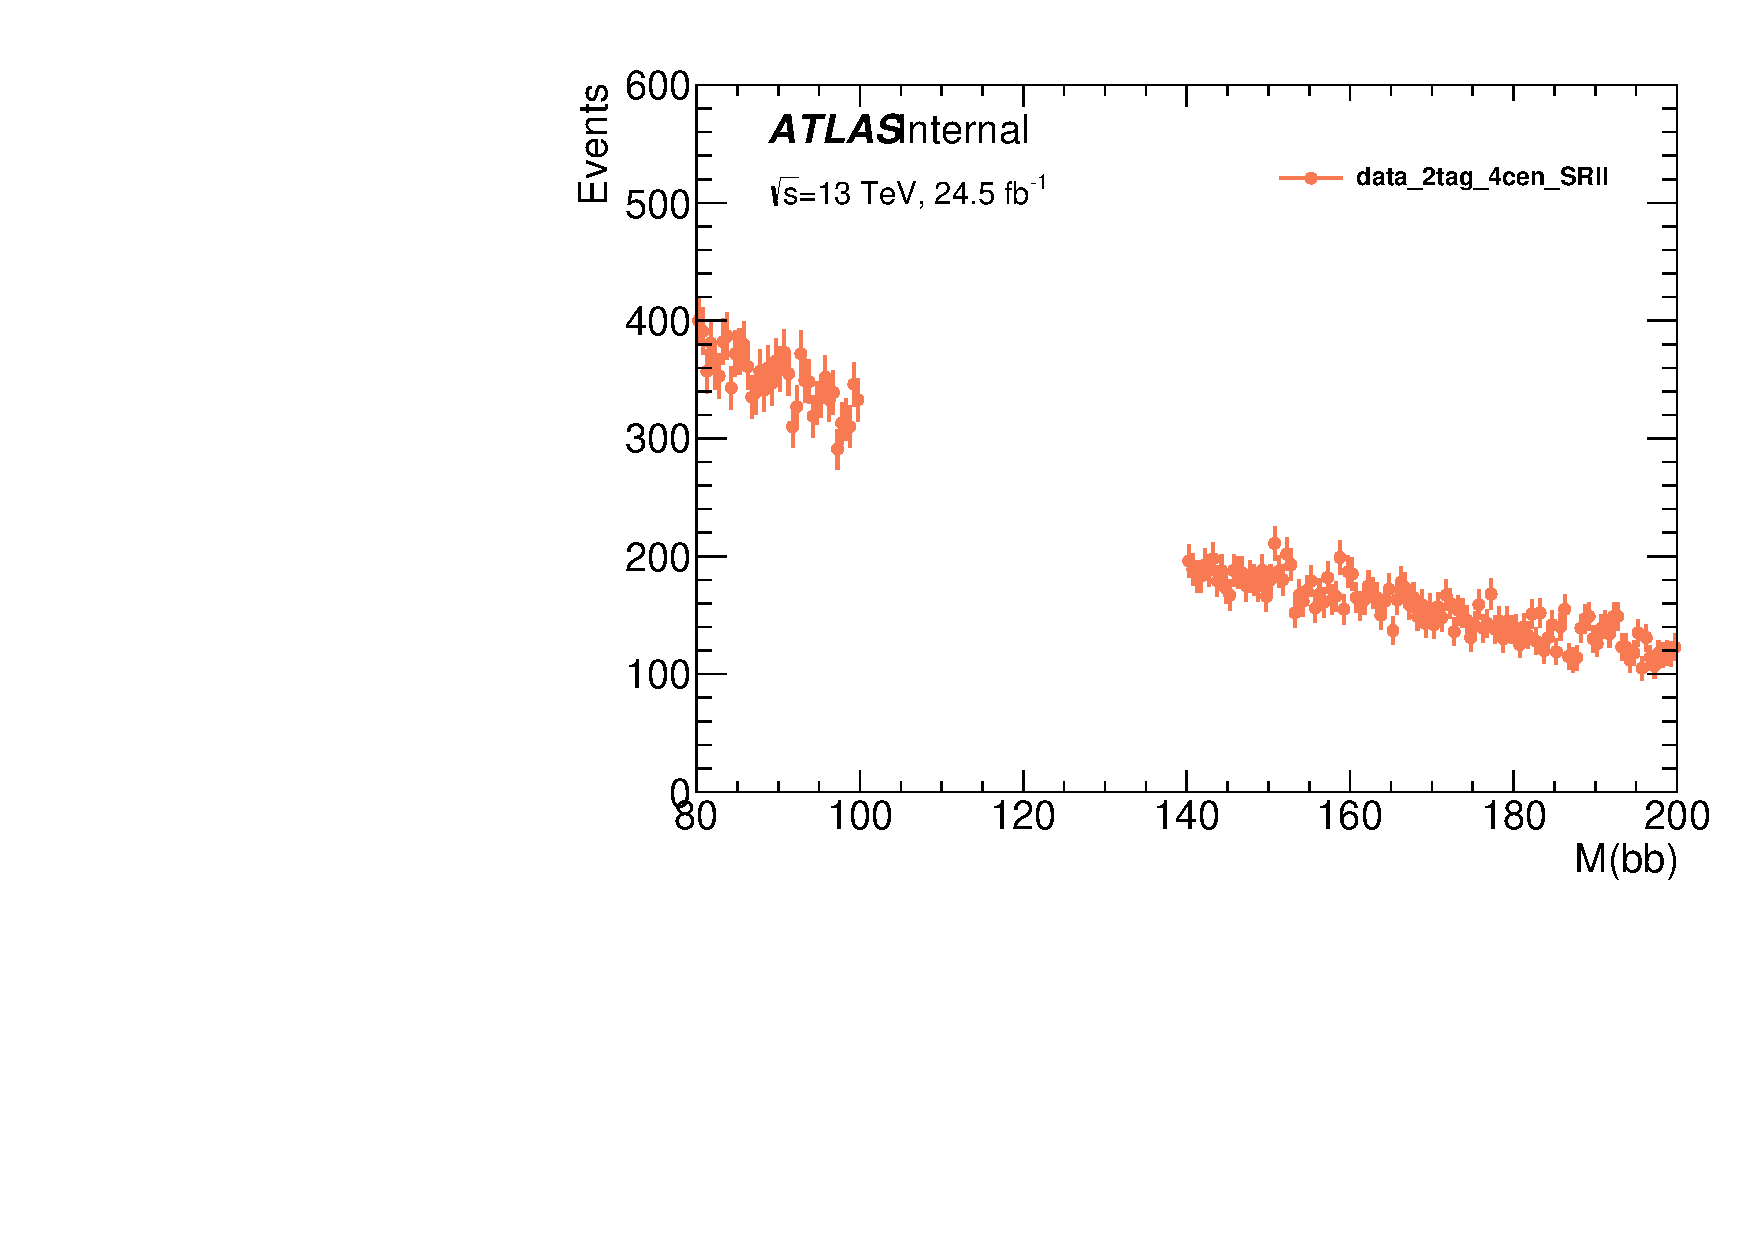
\includegraphics[width=0.45\textwidth]{figures_alt/Mbb_SRII_4cen.pdf}\\
 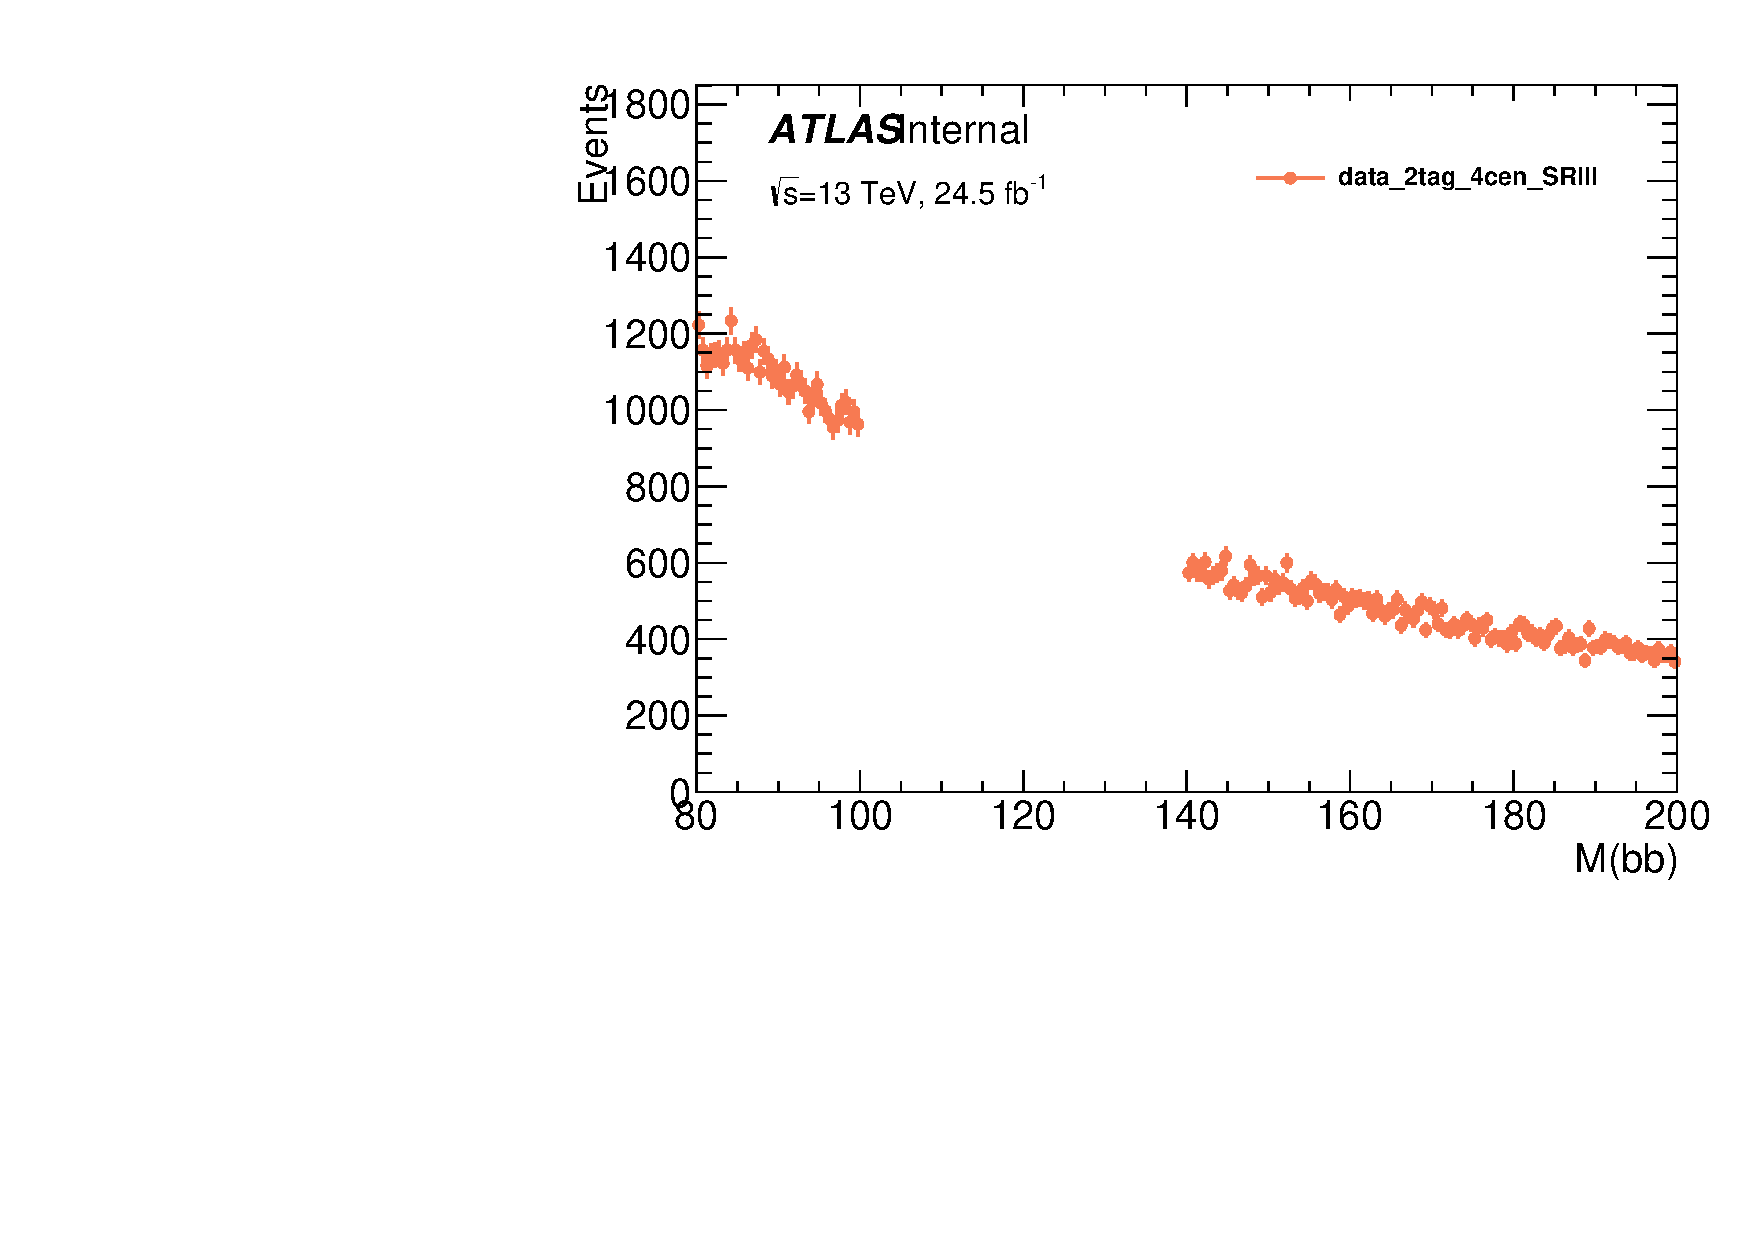
\includegraphics[width=0.45\textwidth]{figures_alt/Mbb_SRIII_4cen.pdf}
 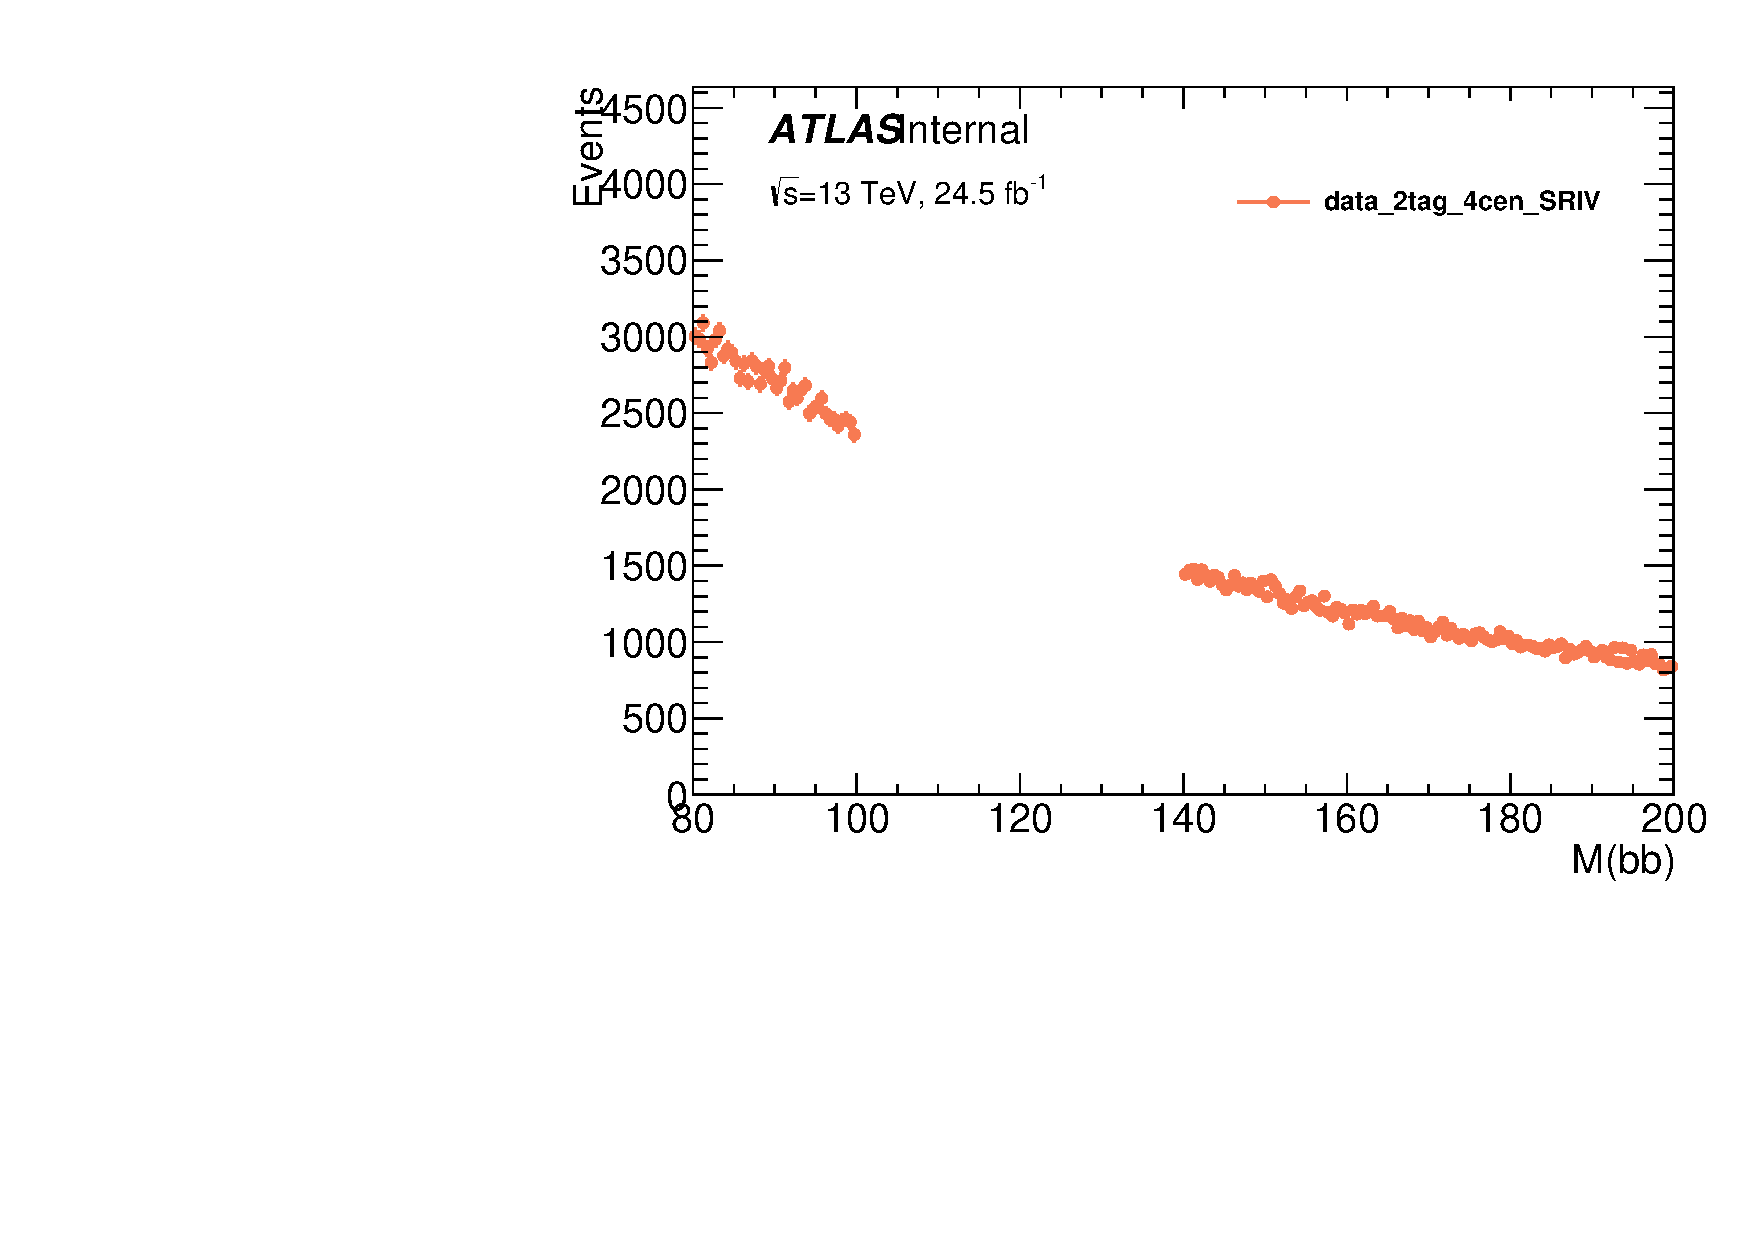
\includegraphics[width=0.45\textwidth]{figures_alt/Mbb_SRIV_4cen.pdf}\\
\caption{\Mbb{} shapes of all BDT regions in sidebands} 
  \label{fig:mbb_sidebands}
\end{figure}


\paragraph{Function choice}

The Bernstein polynomials (defined in Eq. Equation~\ref{eq:bernstein}) are considered and tested, while the exponential times Bernstein polynomial and  sum of exponentials are considered as alternative truth models to derive the spurious signal. 

The functions are required to pass two conditions:

\begin{itemize}
\item (1) Compatibility: The function must be statistically 
compatible with the sidebands of the \Mbb{} distribution in the signal regions,
where the Higgs mass range $100<\Mbb<140$ GeV is ignored. The compatibility criterion is defined as $P(\chi^2)>0.05$ and $P(F-\rm{test})>0.05$, 
where the $\chi^2$ and $F-\rm{test}$ probabilities are considered, respectively.
The $F-\rm{test}$ is performed with respect to the $n+1$ order function.  Only statistical errors are considered in these fits. 
Among the candidates satisfying the conditions above, the function with the smallest
number of degrees of freedom is chosen.
For this study, the \zjets{} component is included in the fit, 
normalized to the SM prediction.

\item (2) Spurious Signal: 
The the lowest order Bernstein polyonominal that satisfies condition (1), $f_{Bern}$, is tested against the the lowest order 
functions in the alternative truth models, $f_{A}$, that also satisfies condition (1) to derive the spurious signal size. 
In other words, we fit the background only hypothesis $f_{A}$ with $f_{Bern}$ plus $\mu_{sp}$ times the signal. The measured  apparent signal size needs to be less than $50\%$ of the actual siganl size. If not, the the next order Bernstein polynomial satisfying condition (1) is tested. 

\end{itemize}


\begin{equation}
\label{eq:bernstein}
\begin{aligned}
\textnormal{Berstein O2} &= a_1(1-k)^2 + 2a_2(1-k)k + a_3k^2, \\
\textnormal{Berstein O3} &= a_1(1-k)^3 + 3a_2(1-k)^2k + 3a_3(1-k)k^2 + a_4k^3, \\
\textnormal{Berstein O4} &= a_1(1-k)^4 + 4a_2(1-k)^3k + 6a_3(1-k)^2k^2 + 4a_4(1-k)k^3 + a_5k^4,\\
\textnormal{Berstein O5} &= a_1(1-k)^5 + 5a_2(1-k)^4k + 10a_3(1-k)^3k^2 + 10a_4(1-k)^2k^3 + 5a_5(1-k)k^4 +a_6k^5, \\
\textnormal{where } k &\equiv \frac{(x-80)}{120}
\end{aligned}
\end{equation}


The $\chi^2$ values and probabilities  and $F-\rm{test}$ probabilities are summarized 
in Tables~\ref{tab:chi2-2cen} ~\ref{tab:chi2-4cen} ~\ref{tab:f-test}.
The $\chi^2$ test criteria are met for the O(2) Bernstein function in all regions, except the in 
SR IV of \fourcentral we need at least O(3) Bernstein function. The $F$-test is passed for for functions
which pass the $\chi^2$ criterion in all channels and regions.

The spurious signal fits are given in Table~\ref{tab:spurious}. Most of the regions will need
at least O(3) Bernstein polynomial.

To summarize, we choose the O(2) Bernstein function for SR I of \twocentral region, O(3) Bernstein 
function for SR II, SR III, SR IV of \twocentral channel and SR I, SR III of \fourcentral channel. 
The other regions will use O(4) Bernstein function.


\begin{table}[]
\centering
\caption{Background Only Fit $\chi^2$ and Prob($\chi^2$) for \twocentral region}
\label{tab:chi2-2cen}
\begin{tabular}{|l|l|l|l|l|l|l|}
\hline
   & \multicolumn{3}{c|}{\twocentral SR I}              & \multicolumn{3}{c|}{\twocentral SR II}             \\ \hline
   & Bernstein   & Expo*Bernstein & Sum of Expo & Bernstein   & Expo*Bernstein & Sum of Expo \\ \hline
O2 & 1.04 (0.37) & 1.06 (0.35)    & 1.04 (0.39)         & 1.16 (0.16) & 1.14 (0.19)    & 1.20 (0.12)         \\ \hline
O3 & 1.06 (0.35) & 0.98 (0.53)    & 1.01 (0.45)         & 1.12 (0.22) & 1.14 (0.19)    & 1.15 (0.17)         \\ \hline
O4 & 0.99 (0.50) & 0.99 (0.50)    & 1.01 (0.33)         & 1.12 (0.23) & 1.14 (0.19)    & 1.20 (0.11)         \\ \hline
O5 & 1.00 (0.49) &                &                     & 1.12 (0.23) &                &                     \\ \hline
   & \multicolumn{3}{c|}{\twocentral SR III}            & \multicolumn{3}{c|}{\twocentral SR IV}             \\ \hline
   & Bernstein   & Expo*Bernstein & Sum of Expo & Bernstein   & Expo*Bernstein & Sum of Expo \\ \hline
O2 & 1.12 (0.21) & 1.12 (0.22)    & 1.12 (0.22)         & 1.02 (0.42) & 0.99 (0.51)    & 0.98 (0.51)         \\ \hline
O3 & 1.11 (0.24) & 1.13 (0.21)    & 1.15 (0.17)         & 0.99 (0.50) & 1.00 (0.48)    & 1.03 (0.41)         \\ \hline
O4 & 1.12 (0.23) & 1.13 (0.21)    & 1.18 (0.14)         & 0.99 (0.51) & 1.00 (0.47)    & 1.04 (0.39)         \\ \hline
O5 & 1.15 (0.17) &                &                     & 0.99 (0.51) &                &                     \\ \hline
\end{tabular}
\end{table}


\begin{table}[]
\centering
\caption{Background Only Fit $\chi^2$ and Prob($\chi^2$) for \fourcentral region}
\label{tab:chi2-4cen}
\begin{tabular}{|l|l|l|l|l|l|l|}
\hline
   & \multicolumn{3}{c|}{\twocentral SR I}              & \multicolumn{3}{c|}{\twocentral SR II}             \\ \hline
   & Bernstein   & Expo*Bernstein & Sum of Expo & Bernstein   & Expo*Bernstein & Sum of Expo \\ \hline
O2 & 0.93 (0.73) & 0.93 (0.73)    & 0.93 (0.73)         & 0.98 (0.55) & 0.96 (0.61)    & 0.97 (0.61)         \\ \hline
O3 & 0.93 (0.73) & 0.93 (0.71)    & 0.94 (0.69)         & 0.96 (0.63) & 0.95 (0.68)    & 0.98 (0.56)         \\ \hline
O4 & 0.93 (0.73) & 0.94 (0.69)    & 0.94 (0.65)         & 0.95 (0.65) & 0.95 (0.66)    & 0.99 (0.52)         \\ \hline
O5 & 0.94 (0.71) &                &                     & 0.95 (0.67) &                &                     \\ \hline
   & \multicolumn{3}{c|}{\twocentral SR III}            & \multicolumn{3}{c|}{\twocentral SR IV}             \\ \hline
   & Bernstein   & Expo*Bernstein & Sum of Expo & Bernstein   & Expo*Bernstein & Sum of Expo \\ \hline
O2 & 1.03 (0.39) & 0.96 (0.62)    & 0.93 (0.73)         & 1.21 (0.04) & 1.06 (0.29)    & 1.06 (0.29)         \\ \hline
O3 & 0.96 (0.62) & 0.97 (0.58)    & 0.94 (0.69)         & 1.08 (0.23) & 1.07 (0.26)    & 1.07 (0.25)         \\ \hline
O4 & 0.97 (0.61) & 0.98 (0.55)    & 0.98 (0.55)         & 1.06 (0.28) & 1.06 (0.30)    & 1.08 (0.24)         \\ \hline
O5 & 0.96 (0.63) &                &                     & 1.05 (0.31) &                &                     \\ \hline
\end{tabular}
\end{table}



\begin{table}[]
\centering
\caption{Background Only Fit F-test}
\label{tab:f-test}
\begin{tabular}{|l|l|l|l|l|l|l|l|l|}
\hline
                          & \multicolumn{4}{c|}{\twocentral} & \multicolumn{4}{c|}{\fourcentral} \\ \hline
Region                    & SR I  & SR II  & SR III  & SR IV & SR I  & SR II  & SR III  & SR IV  \\ \hline
Bernstein O2/ O3          & 0.51  & 0.45   & 0.48    & 0.46  & 0.50  & 0.44   & 0.34    & 0.14   \\ \hline
Bernstein O3/ O4          & 0.44  & 0.51   & 0.50    & 0.50  & 0.52  & 0.49   & 0.51    & 0.42   \\ \hline
Bernstein O4/ O5          & 0.51  & 0.50   & 0.51    & 0.50  & 0.52  & 0.48   & 0.48    & 0.46   \\ \hline
Sum of Expo O2/O3 & 0.44  & 0.52   & 0.53    & 0.53  & 0.55  & 0.53   & 0.53    & 0.52   \\ \hline
Sum of Expo O3/O4 & 0.54  & 0.53   & 0.53    & 0.53  & 0.55  & 0.53   & 0.52    & 0.45   \\ \hline
Expo*Bernstein O2/O3      & 0.43  & 0.50   & 0.51    & 0.52  & 0.52  & 0.53   & 0.49    & 0.56   \\ \hline
Expo*Bernstein O3/O4      & 0.52  & 0.52   & 0.51    & 0.50  & 0.52  & 0.53   & 0.52    & 0.34   \\ \hline
\end{tabular}
\end{table}

\begin{table}[]
\centering
\caption{Background spurious signal test for \twocentral region}
\label{tab:spurious-test-2cen}
\begin{tabular}{|c|c|c|c|c|}
\hline
             & \multicolumn{2}{c|}{SR I}                  & \multicolumn{2}{c|}{SR II}                 \\ \hline
             & Expo*Bernstein O2 & Sum of Expo O2 & Expo*Bernstein O2 & Sum of Expo O2 \\ \hline
Bernstein O2 & \textless0.01     & 0.45                   & 6.1               & 2.8                    \\ \hline
Bernstein O3 & \textless0.01     & 0.02                   & 0.33              & 0.14                   \\ \hline
             & \multicolumn{2}{c|}{SR III}                & \multicolumn{2}{c|}{SR IV}                 \\ \hline
             & Expo*Bernstein O2 & Sum of Expo O2 & Expo*Bernstein O2 & Sum of Expo O2 \\ \hline
Bernstein O2 & 1.9               & 2.3                    & 10.2              & 10.7                   \\ \hline
Bernstein O3 & 0.24              & 0.01                   & 0.13              & 0.08                   \\ \hline
\end{tabular}
\end{table}


\begin{table}[]
\centering
\caption{Background spurious signal test for \fourcentral region}
\label{tab:spurious-test-4cen}
\begin{tabular}{|c|c|c|c|c|}
\hline
             & \multicolumn{2}{c|}{SR I}                  & \multicolumn{2}{c|}{SR II}                 \\ \hline
             & Expo*Bernstein O2 & Sum of Expo O2 & Expo*Bernstein O2 & Sum of Expo O2 \\ \hline
Bernstein O2 & 2.3               & 3.1                    & 9.3               & 5.8                    \\ \hline
Bernstein O3 & \textless0.01     & 0.06                   & 0.19              & 1.0                    \\ \hline
Bernstein O4 &                   &                        & 0.18              & 0.25                   \\ \hline
             & \multicolumn{2}{c|}{SR III}                & \multicolumn{2}{c|}{SR IV}                 \\ \hline
             & Expo*Bernstein O2 & Sum of Expo O2 & Expo*Bernstein O2 & Sum of Expo O2 \\ \hline
Bernstein O2 & 1.9               & 2.3                    & 10.2              & 10.7                   \\ \hline
Bernstein O3 & 0.37              & 0.03                   & 0.46              & 1.2                    \\ \hline
Bernstein O4 &                   &                        & 0.46              & 0.08                   \\ \hline
\end{tabular}
\end{table}


\clearpage

\subsubsection{Treatment of \zjets{} contribution}
\label{sec:ztreat}

The \zjets{} contribution plays an important role in the overall fitting procedure due to the fact that it comprises a significant fraction lower \Mbb{} sideband ( 5--6(3--4)\% of the \fourcentral(\twocentral) selection) , yet the sideband does not extend to low enough \Mbb{} values to reliably constrain its contribution using the shape templates.  Therefore, the non-resonant background fit can be partially compensated by the $Z$-yield and vice-versa.  To mitigate the impact of this degeneracy, we could fix the contributions of \zjets{} in the fits to predictions from MC.  However, our \zjets{} MC is only leading order ($Z+$2 partons), and large or varying $k$-factors may be present in the different BDT regions. Hence, multiple strategies are considered for the treatment of \zjets{} contirbutions. 

\begin{enumerate}

\item Use \zjets{} theoretical uncertainties to account for the potential BDT shape difference: We lack the systematics variation samples ($\alpha_s$, renomalization scale) to compute the theoretical uncertainties. Nor do we have \zjets{} samples from other generators. This approach is not feasible for the current round of analysis. 

\item Use data to MC \zmujets{} as scale factor for \zjets{} BDT shape: Since the BDT input variables are largely indepedent of the $Z$ decay process, we can select a pure \zmujets{} sample in data and MC to determine the not only the accuracy of modeling of the \zjets{} BDT shape but also the total cross section of $Z$ production in data after the pre-selection. This method would be valid if we also observe a closure in the ratio of $\frac{\zjets{}(MC)}{\zmujets{}(MC)}$. The details of the \zmujets{} selection and study are found in Appendix~\ref{sec:app-zmm}.  Cuts are applied to the dimuon $Z$-candidate to emulate the di-\bjet selection of the Higgs candidate. The cross-section ratios of data to MC after pre-selection are calculated to be 0.81$\pm$0.06 and 0.75$\pm$0.06 for \twocentral and \fourcentral channels respectively. The errors include the statistical uncertainties on the data and MC. The relative ratios of the number of events in data and MC, and between \zjets{} and \zmujets{} MC are shown in Table~\ref{tab:z_ratios} for all of the regions considered in the analysis. However, notably the \zmujets{} to \zjets MC ratio is not close to one in some regions, which may be due to the fact that different generators are used for the electro-weak production events, or due to residual differences in the \bjet and muon events arising from a different mis-tag rate and different final state QCD radiation effects. Hence applying the scale factors we derived from \zmujets{} study may not be directly applicable to \zjets{}. 

\item Use two-point uncertainty for \zjets{} process: From the injection study (Appendix~\ref{sec:app-zmm}) one could also quote an uncertainty of $mu_H$ due to the variation of $Z$ contribution independent of other systematics. However the method can not profile the $Z$ systematics in the likelihood fit. 

\item \label{item:z-treat-4} Float the contribution of $Z$ in all BDT regions: Assume no prior knowledge of $Z$ contribution in all BDT regions and allow the contribution to float in the profile likelihood fit: This is the most conservative strategy and yields the largest systeamtics. 

\item \label{item:z-treat-5} Float the contribution of $Z$ in SR I and SR II of \twocentral channel and the total cross section of $Z$; Constrain the $Z$ shape variation to 50\% of the \zjets{} MC for all other BDT regions: Besides the SR I and SR II of the \twocentral channel, all other BDT regions we have reasonalbe constraints as shown in \ref{tab:z_ratios}. We know for these regions, we have good clusre between \zjets{} and \zmujets{} MC as well as smal difference across \zmujets{} MCs. Therefore the \zmujets{} data to MC ratios are applicable to \zjets{}. We also know the ratios $\frac{\zmujets{}(Data)}{\zmujets{}(MC)}$ are close to one, hence we can quote the difference between 1 and $\frac{\zmujets{}(Data)}{\zmujets{}(MC)}$ as systematics. To be conservative, we quote 50\% shape variations for all these regions. This method yields smaller systematics than the strategy of floating all $Z$ contributions. 

\end{enumerate}



\begin{table}[]
\centering
\caption{Relative Ratios of $\frac{\zmujets{}(Data)}{\zmujets{}(MC)}$, 
$\frac{\zjets{}(MC)}{\zmujets{}(MC)}$ 
and $\frac{\zmujets{}(\textnormal{Powheg})}{\zmujets{}(\textnormal{Madgraph})}$}
\label{tab:z_ratios}
\begin{tabular}{|l|r|r|r|}
\hline
Region       &  $\frac{\zmujets{}(Data)}{\zmujets{}(MC)}$ & $\frac{\zjets{}(MC)}{\zmujets{}(MC)}$ & $\frac{\zmujets{}(\textnormal{Powheg})}{\zmujets{}(\textnormal{Madgraph})}$  \\ \hline
SR I   (2cen)  & 0.73 (0.14) & 0.35 (0.10) & 1.06 (0.28)\\ \hline
SR II  (2cen)  & 0.50 (0.08) & 0.54 (0.10) & 1.40 (0.35)\\ \hline
SR III (2cen)  & 0.91 (0.09) & 1.03 (0.12) & 0.95 (0.14)\\ \hline
SR IV  (2cen)  & 1.16 (0.07) & 1.14 (0.08) & 0.97 (0.09)\\ \hline
SR I   (4cen)  & 0.82 (0.06) & 0.74 (0.08) & 1.00 (0.11)\\ \hline
SR II  (4cen)  & 0.83 (0.05) & 0.95 (0.09) & 0.89 (0.08)\\ \hline
SR III (4cen)  & 0.96 (0.03) & 1.05 (0.04) & 1.07 (0.06)\\ \hline
SR IV  (4cen)  & 1.06 (0.02) & 1.01 (0.03) & 0.99 (0.04)\\ \hline

\end{tabular}
\end{table}



%\subsection{Uncertainties}
%\label{sec:uncertainties}
%-------------------------------------------------------------------------------
%\label{sec:vbf-uncertainties}

Several sources of systematic uncertainties,
affecting the normalization of signal and background and/or the shape of
the distributions used in this analysis, have been considered.  Individual sources of systematic 
uncertainty are considered uncorrelated. The systematic variations with less than $0.5\%$ impact 
on the yields in a particular BDT region will be ignored in the profile likelihood fit for 
that particular region. 

\subsubsection{Luminosity}
\label{sec:vbf-syst_lumi}

The integrated luminosity measurement has an uncertainty of 3.4\%. This systematic uncertainty
is applied to all physics processes estimated with MC simulated samples normalized 
to the measured integrated luminosity: \zjets{} and Higgs production. {\it Ed. Note: this will be updated after the unblinding.}

\subsubsection{Uncertainties on object definitions}
\label{sec:vbf-syst_objects}

Several uncertainties are applied to the MC simulation samples to take into account the limited knowledge of the detector and reconstruction performance.

\paragraph{Trigger efficiencies}

The per-jet online b-tagging efficiency with respect to the offline b-tagging efficiency is measured in $t\bar t$ events. 
To cover the event topology dependence, a scale factor applied to the leading b-tagged jet is derived as a function of the jet $\eta$. 

\paragraph{JVT efficiency}
The per-jet efficiency to satisfy the jet vertex tagging requirement
is measured in $Z(\to \ell^+\ell^-)$+1-jet events in data and simulation,
selecting separately events enriched in hard-scatter jets and events enriched in pile-up jets. 
The corresponding uncertainty is evaluated by shifting the per-jet scale factors,
accounting for the efficiency uncertainty~\cite{JVTwiki}.

\paragraph{Jet energy scale}
%\label{sec:vbf-syst_jes}
The jet energy scale and its uncertainty have been derived combining information from test-beam data, 
LHC collision data and simulation \cite{JESwiki}. The jet
energy scale uncertainty is split into 4 uncorrelated sources, 
which can have different jet $\pt$ and $\eta$ dependencies.  These sources are
treated independently in this analysis, using the \texttt{JetUncertainties} tool \cite{TWiki_JetUncertainties} 
to compute the uncertainties corresponding to each eigenvector. 
The variation in the jet energies as a result of these systematic uncertainties are also propagated through all
observables computed using jet kinematics.

\paragraph{Jet energy resolution}
%\label{sec:vbf-syst_jer}
[The jet energy resolution (JER) has been measured separately for data and simulation 
using in-situ techniques. The \texttt{JERUncertaintyProvider}
tool~\cite{jeruncertaintyprovider} was used to obtain the expected fractional
$p_T$ resolution for a given jet as a function of its $p_T$ and rapidity. 
The systematic uncertainty is taken by smearing the jet energy by the shift 
in resolution provided by the tool and comparing to the nominal
shape and normalization in simulation. 
The nominal value is used as the default in the analysis.

In order to propagate the uncertainty in the $p_T$ resolution, for each jet a 
random number $r$ is drawn from a Gaussian distribution with mean 0 and sigma equal 
 to the difference in quadrature between the fractional $p_T$ resolution with the tool and the nominal
one.  The jet 4-momentum is then scaled by a factor $1+r$.  By definition, such uncertainty
is one-sided, since jets in simulation cannot be under-smeared. 
We compute the normalization and shape uncertainties in the final distributions 
and symmetrize them to define a corresponding "down'' variation.

\paragraph{\btagging}
%\label{sec:vbf-syst_btag}

The effects of uncertainties in efficiencies for the heavy flavor tagging of jets by
the MV2c10 tagger have been evaluated. This analysis uses the operating points 
with approximately 60\%, 70\% and 85\% efficiency for $b$-quark jets. 
These efficiencies are measured
from data for each jet flavor.

Simulation efficiencies for $b$ and $c$ quarks have to be corrected by a
$\pt$-dependent factor. In the case of light flavor jets, the corrections also 
depend on jet $\eta$. 
Each uncertainty corresponds to a resulting eigenvector after diagonalizing the matrix
containing the information of total uncertainty per $\pt$ bin and the bin-to-bin 
corrections. These systematic
uncertainties are taken as uncorrelated between $b$, $c$, and light flavor jets.
A per-jet weighting procedure is applied to simulated events to propagate the 
calibration of $b$-tagging and the related uncertainties. 
The correlation across operating points is ignored. It has been checked that this choice
wouldn't impact the results by considering the uncertainties fully correlated or fully uncorrelated.


\paragraph{Track multiplicity for Quark/gluon separation}

The track multipicity discrimination power for quark/gluon separation in simulation 
is affected by the modeling of the charged multiplicity in jet fragmentation and the modeling of the
track multiplicity reconstruction. The estimation of the corresponding uncertainties is 
described in Ref.~\cite{qgtagging}. A total of 5 nuisance parameters is used to parametrize these
uncertainties and the impact on the results presented in this note is found to be negligible.

\subsubsection{Analytical and Theoretical Modeling uncertainties of signal}
\label{sec:vbf-syst_model}

Uncertainties in the modeling both of the non-resonant background shape and the theory and phenomenological modeling uncertainties of the Monte Carlo simulation samples are described here.


\paragraph{Non-resonant background}
The non-resonant background is modeled with an analytical function, either O(3) or O(4) Bernstein polynomial. 
The potential local bump or dip caused by the functional choice is characterized by spurious signal 
which is derived by fitting the nominal model plus signal to an alternative model. The derived spurious signal 
size is then quoted the width of a gaussian constraint which is included in the profile likelihood as in 
Eq.~\ref{likelihood}.

%\paragraph{\zjets{} normalization}
%\label{sec:vbf-zjets}
%
%Strategy~\label{item:z-treat-5} of section~\ref{sec:vbf-ztreat} is taken for the systematic uncertainties on the \zjets{} normalization.
%
%The bias on the signal $\mu$ value caused by this rescaling (or lack thereof) is estimated 
%with an injection test where the scaled pseudodata is fit with the non-scaled template. 
%The bias is found to be less than $10\%$ and therefore negligible with respect to the overall uncertainty.
%Therefore no relative rescaling is applied to the \zjets{} MC prediction in each region.
%Additional details of these studies are provided in Appendix ~\ref{sec:vbf-app-zmm}.

%The normalization of the \zjets{} background, simulated at LO, is 
%affected by potentially large uncertainties~\cite{zkfactors}. 
%In order to estimate the \zjets{} normalization in data, the $Z(\mu\mu)+$jets yield
%is used as proxy. The ratio between data and MC yield after preselection is used to estimate the overall
%normalization and the difference between \zjets{} and $Z(\mu\mu)+$jets is 
%taken as uncertainty.
%The data/MC ratio is found to be 0.74(0.1) and 0.79(0.1) for \twocentral and \fourcentral channels respectively. 
%A single gaussian NP with width 0.1 is therefore used in the global fit. 
%The $Z(\mu\mu)+$jets sample is also used to study the variation across signal and control regions.
%The \zjets{} prediction is scaled in each BDT region by the ratios between the yields observed in $Z(\mu\mu)+$jets data
%and in \zjets{} and $Z(\mu\mu)+$jets MC. The scale factors are listed in Table~\ref{tab:z_ratios}
% 

\paragraph{QCD Scale Variations}

The QCD scale uncertainty for VBF is taken as varying the renormalization
and factorization scales together by a factor of 2 and 0.5. As indicated in ~\cite{QCDscale_vbf}, 
this treatment in general leads to larger variations than the independent variation of renormalization
and factorization scales. 

The QCD scale uncertainty for ggF follows the \textit{2017 scheme} recommended by 
WG1 in the follow-up of March meeting 2017 ~\cite{QCDscale_ggF}. In total, nine independent 
variations in six categories are considered. The terms and corersponding uncertainty sources 
are the following:

\begin{enumerate}
\item \textit{mu}, factorization scale variation
\item \textit{res}, renormalization scale variation
\item \textit{vbf2j} and \textit{vbf3j}, VBF topology uncertainties
\item \textit{mig01} and \textit{mig12}, truth level bin migration for non-Higgs jets
\item \textit{pTH60} and \textit{pTH120}, uncertainties extrapolation with Higgs $p_T$
\item \textit{qmt}, uncertainties of top quark mass
\end{enumerate}

The dominant source of uncertainty for this analysis comes from the term \textit{mig12} (size of $~17-18\%$), 
which is the leading source of uncertainty in high $p_T(H)$ event topology. 

Naively, one would assume uncertainties due to VBF topology terms are considerable. 
However, it is worth noting that these terms only matter for events which 
at truth level are generated in VBF topology. An event falls into Stage one classification 
of VBF topology if the truth Higgs has $p_T<200GeV$ and 
\begin{enumerate}
\item $MJJ>400 GeV$ and $|\textnormal{rapidity(J1)-rapidity(J2)}|>2.8$ ( loose VBF, events having >3 jets),
\item Pass loose VBF selection $\overrightarrow{p_{T}}(J1)+\overrightarrow{p_{T}}(J2)+\overrightarrow{p_{T}}(Higgs)<25GeV$ (tight VBF, events having ~2 jets),
\end{enumerate}
where the VBF jets are defined as the leading two jets aside from the Higgs. We note that $80\%$ of the events have $p_T(H)>200GeV$ and 
these events would not fall into the VBF category. Hence, the VBF topology uncertainties would not even apply in the \textit{2017 scheme} for most of our events. 
For our application, we could extend the definition of VBF topology to high $p_T(H)$ events and take the \textit{vbf2j} and \textit{vbf3j} values
for low $p_T(H)$ VBF topology to be the uncertainty for high $p_T(H)$ events as well. (\textit{vbf2j} and \textit{vbf3j} are defined as constants.)

We also notice that the \textit{2017 scheme} has a different definition of VBF jets, which selects the leading two jets aside from Higgs,  from the 
offline selection we apply in this analysis, which seeks a pair of jets that maximizes the $MJJ$ value. Hence if an event which is categorized by \textit{2017 scheme}
as non-VBF, the scheme lacks a term to properly count the 2J VS. 3J truth event topology uncertainty. Therefore, we also propagate the VBF topology 2J VS. 3J
uncertainties to standard non-VBF ggF+GE2j category. 

Overall, if VBF topology uncertainties are only applied to low $p_T(H)$ events, this source 
of ucnertainty is $<3\%$ in all signal regions. If the uncertainty is extended to high $p_T(H)$ events and as well as non-VBF ggF+GE2j events, the uncertainty
is about $20\%$. We take this conservative extended version of uncertainty for ggF events.

%\begin{table}[htbp]
%\centering
%\caption{Fraction of ggF events in high $p_T(H)$ and VBF topology category}
%\label{tab:highpTfraction}
%\begin{tabular}{|l|l|l|l|l|l|l|}
%Region   & 2cen SR I & 2cen SR II & 4cen SR I & 4cen SR II & 4cen SR III & 4cen SR IV \\
%Fraction & 17.5\%    & 10.4\%     & 13.2\%    & 19.4\%     & 8.8\%       & 9.5\%     
%\end{tabular}
%\end{table}


\paragraph{PDF}
The uncertainty on the PDF description used to simulate the signal is evaluated
by varying the PDF based on the uncertainties along each of the PDF eigenvectors.
Each variation is applied by reweighting the signal samples event-by-event.
A single nuisance parameter, corresponding to the envelope of all the variations,
is considered.

\paragraph{Parton Shower}

The modeling of parton shower could directly affect observables which are heavily 
correlated with the jettiness of the event. In this analysis, its impact is most 
prominent on $p_{T}$ balance, which is a variable used as the BDT input. The nominal
Pythia sample is compared with the \herwig{} sample at the truth level to derive a 
reweighting map for $p_{T}$ balance.
This reweighting map is then applied to the observable of the reconstructed events. The full impact of this variation 
is evaluated by running the BDT analysis while fixing other variables at their nominal 
and applying reweighting of $p_{T}$ balance. 


\paragraph{Signal Contamination from \VH and \ttH Processes}

The cross section of other Higgs production mode like \VH and \ttH are comparable to
the VBF process. Events from \VH (fully hadronic final states) and \ttH production could 
also pass the event selections of this analysis. The \Mbb distributions of these process
 are shown in Figure~\ref{fig:Mbb-ttH-VH}. The yields of these processes are presented 
in Table~\ref{tab:vh-tth-yield}.  The contributions to the total Higgs yields are  small 
in the most sensitive signal regions (0.2 -- 0.8 \%),  and rise to 15\% in the least sensitive regions.  

The VH process has a prominent resonance peak, similar to the VBF and ggF distributions. However, 
the statistics of the Monte Carlo sample is low, especially in \twocentral channel. 
We assign a 100\% uncertainty to the \VH process yield for a conservative estimate of 
the \VH contribution. %Its yield is added to the Higgs yields from VBF and ggF processes.

The \ttH mass distribution is a combination of the resonance peak and a continuum. 
The continuum arises from the fact that the \ttH process has at least four $b$-jets in the final state.
The failure of the jet assignment to identify the correct Higgs daughter $b$-jets results in a 
continuum combinatorial background which can be clearly seen in Figure~\ref{fig:Mbb-ttH-VH}. 
The yield is also assigned with 100\% uncertainty.
%In the fit, we take the actual shape of \ttH treating it as a background. 


\begin{figure}[htbp]
  \centering
 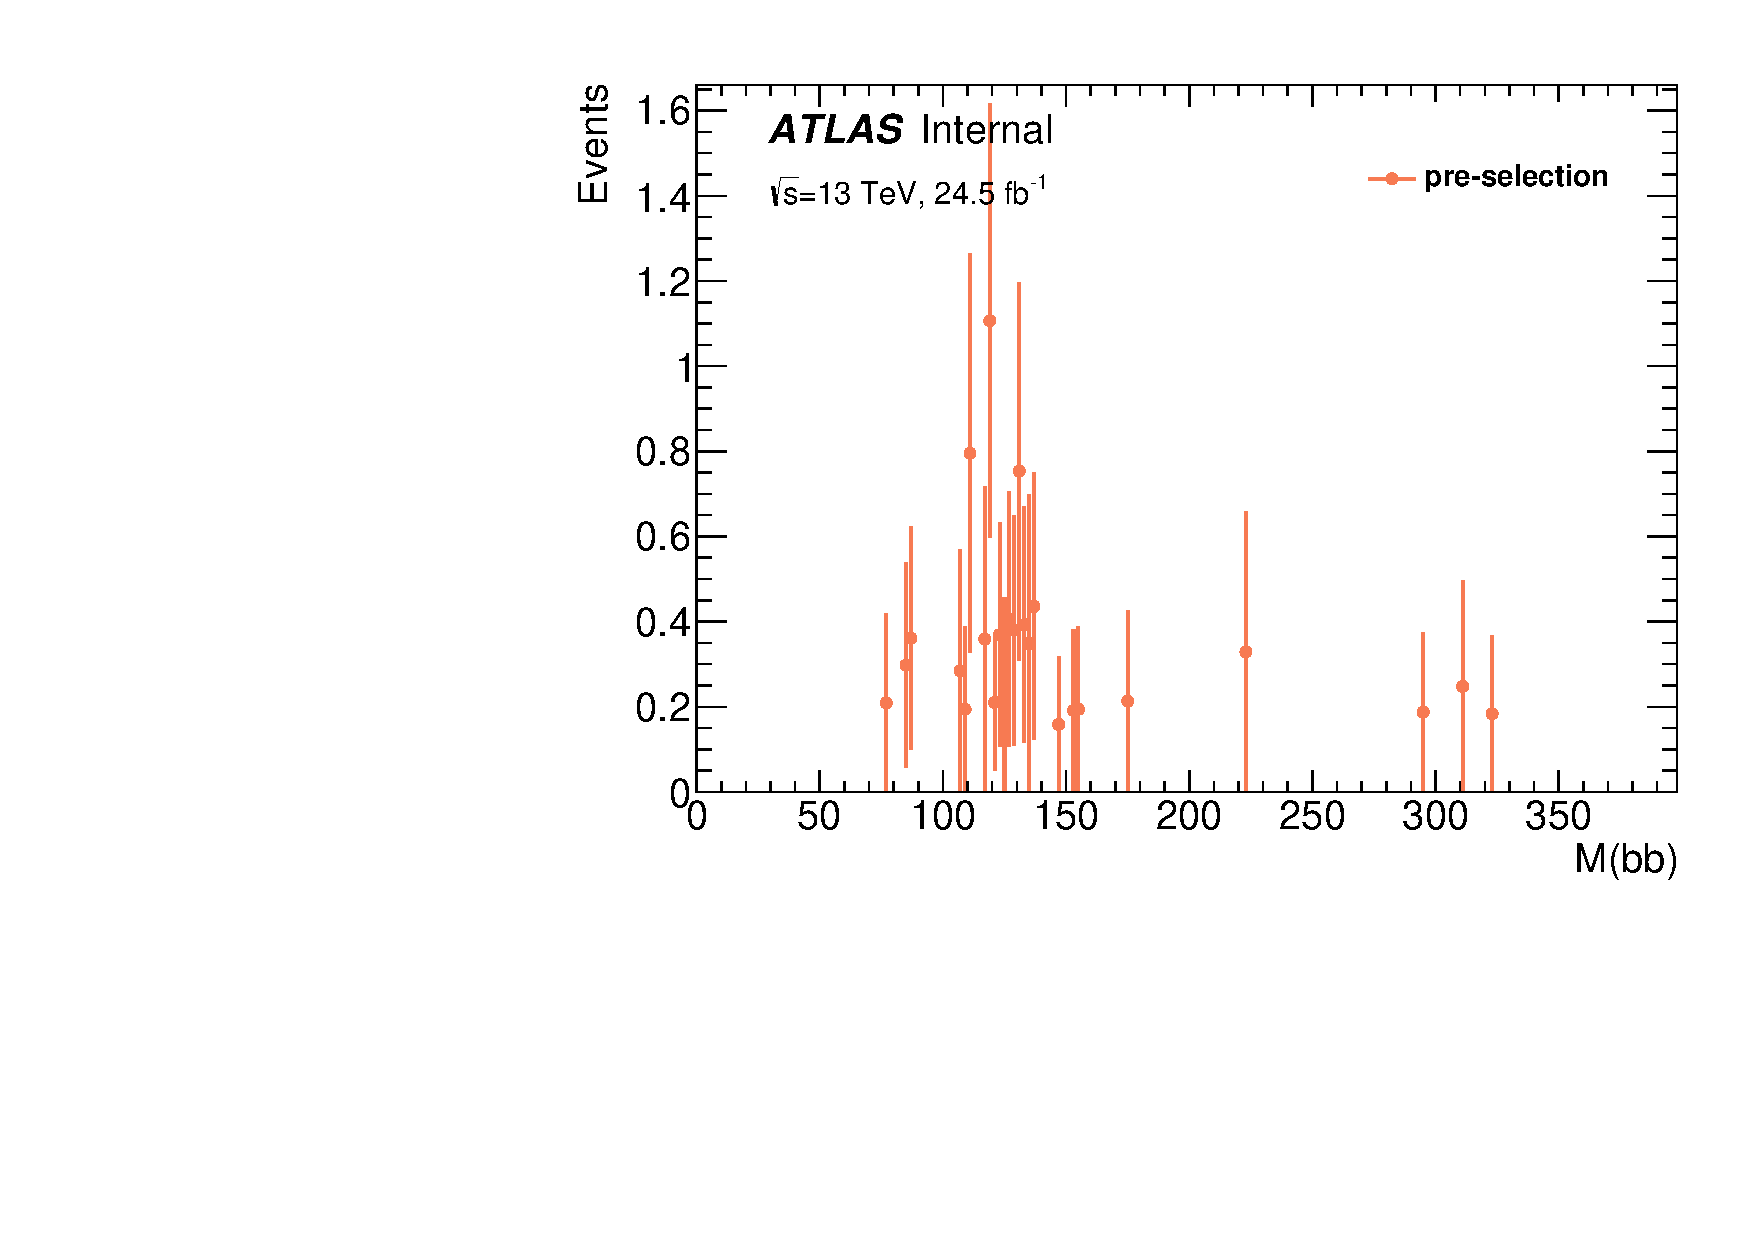
\includegraphics[width=0.42\textwidth]{figures/VBF/Mbb_VH_2cen.pdf}
 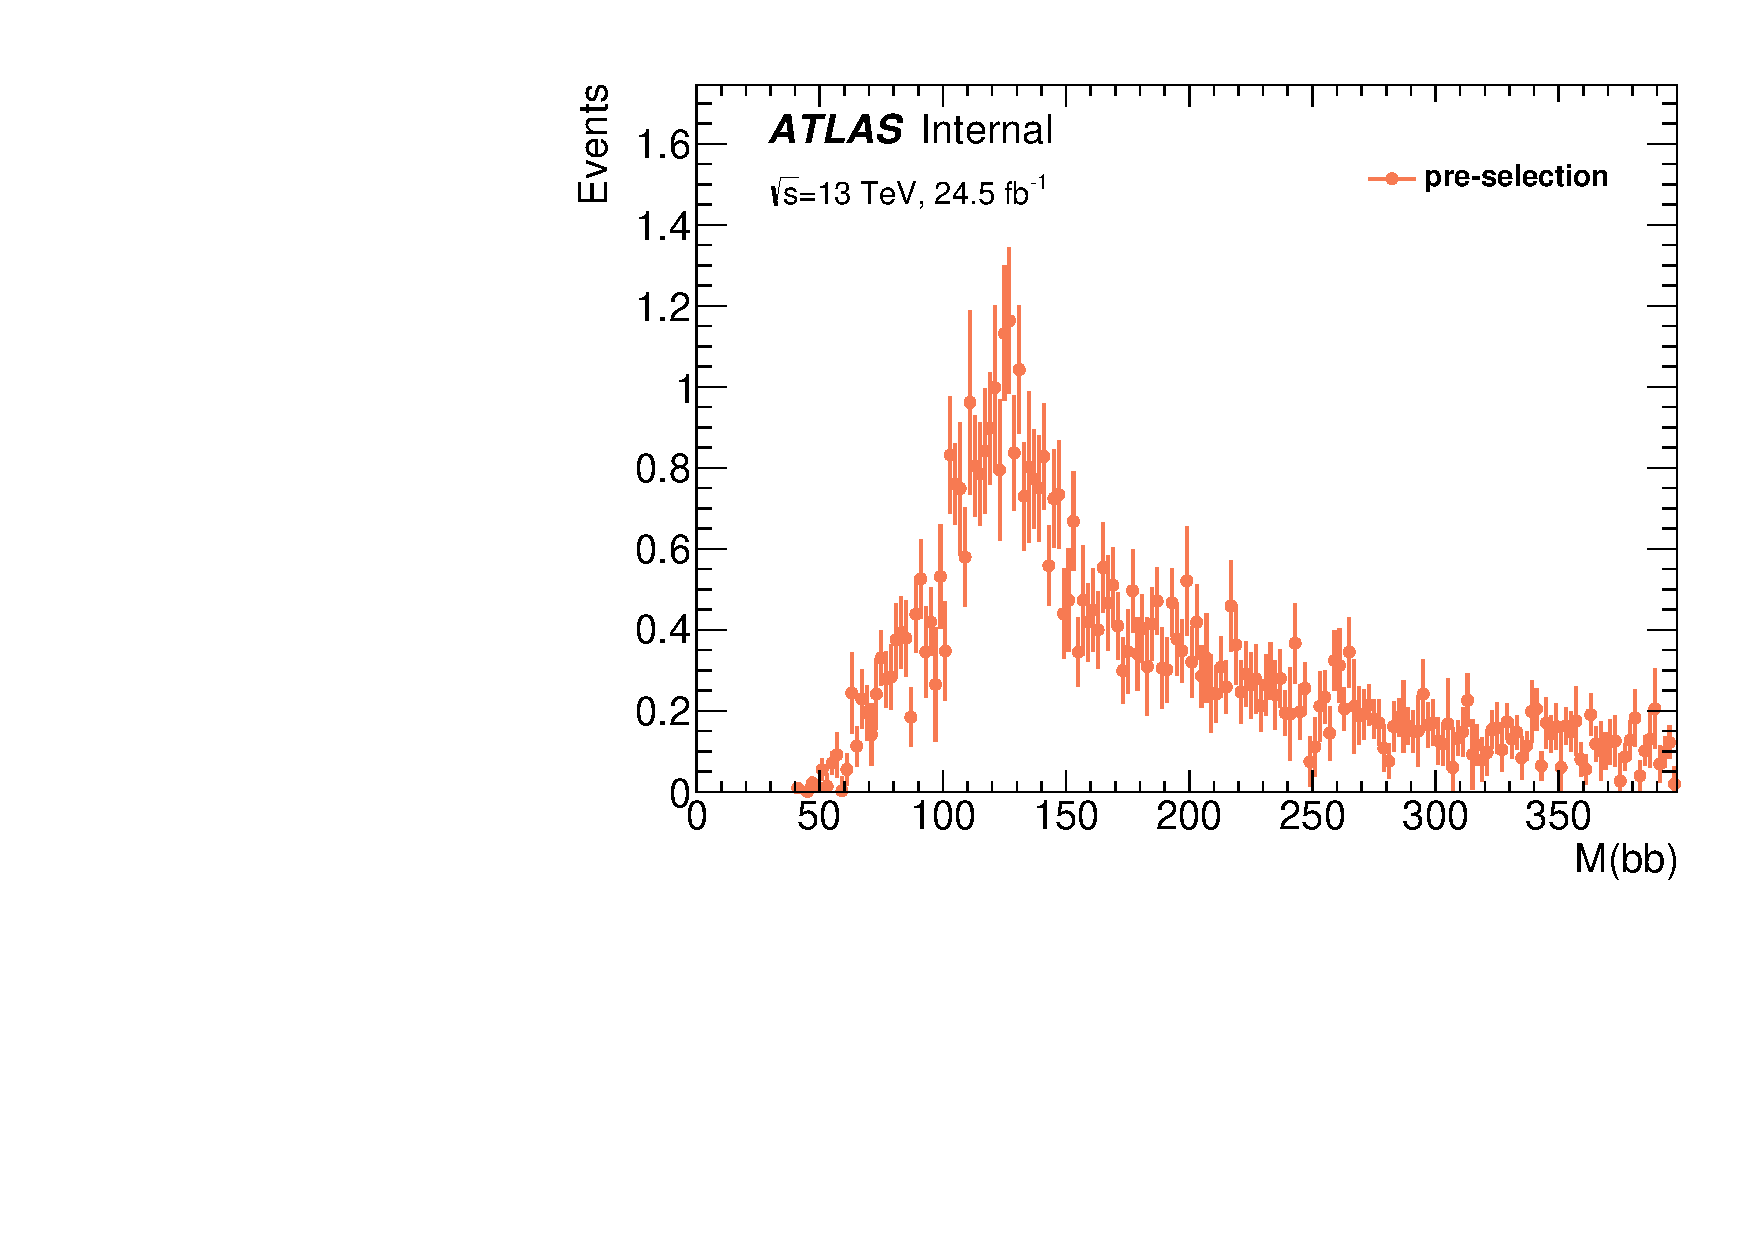
\includegraphics[width=0.42\textwidth]{figures/VBF/Mbb_ttH_2cen.pdf}\\
 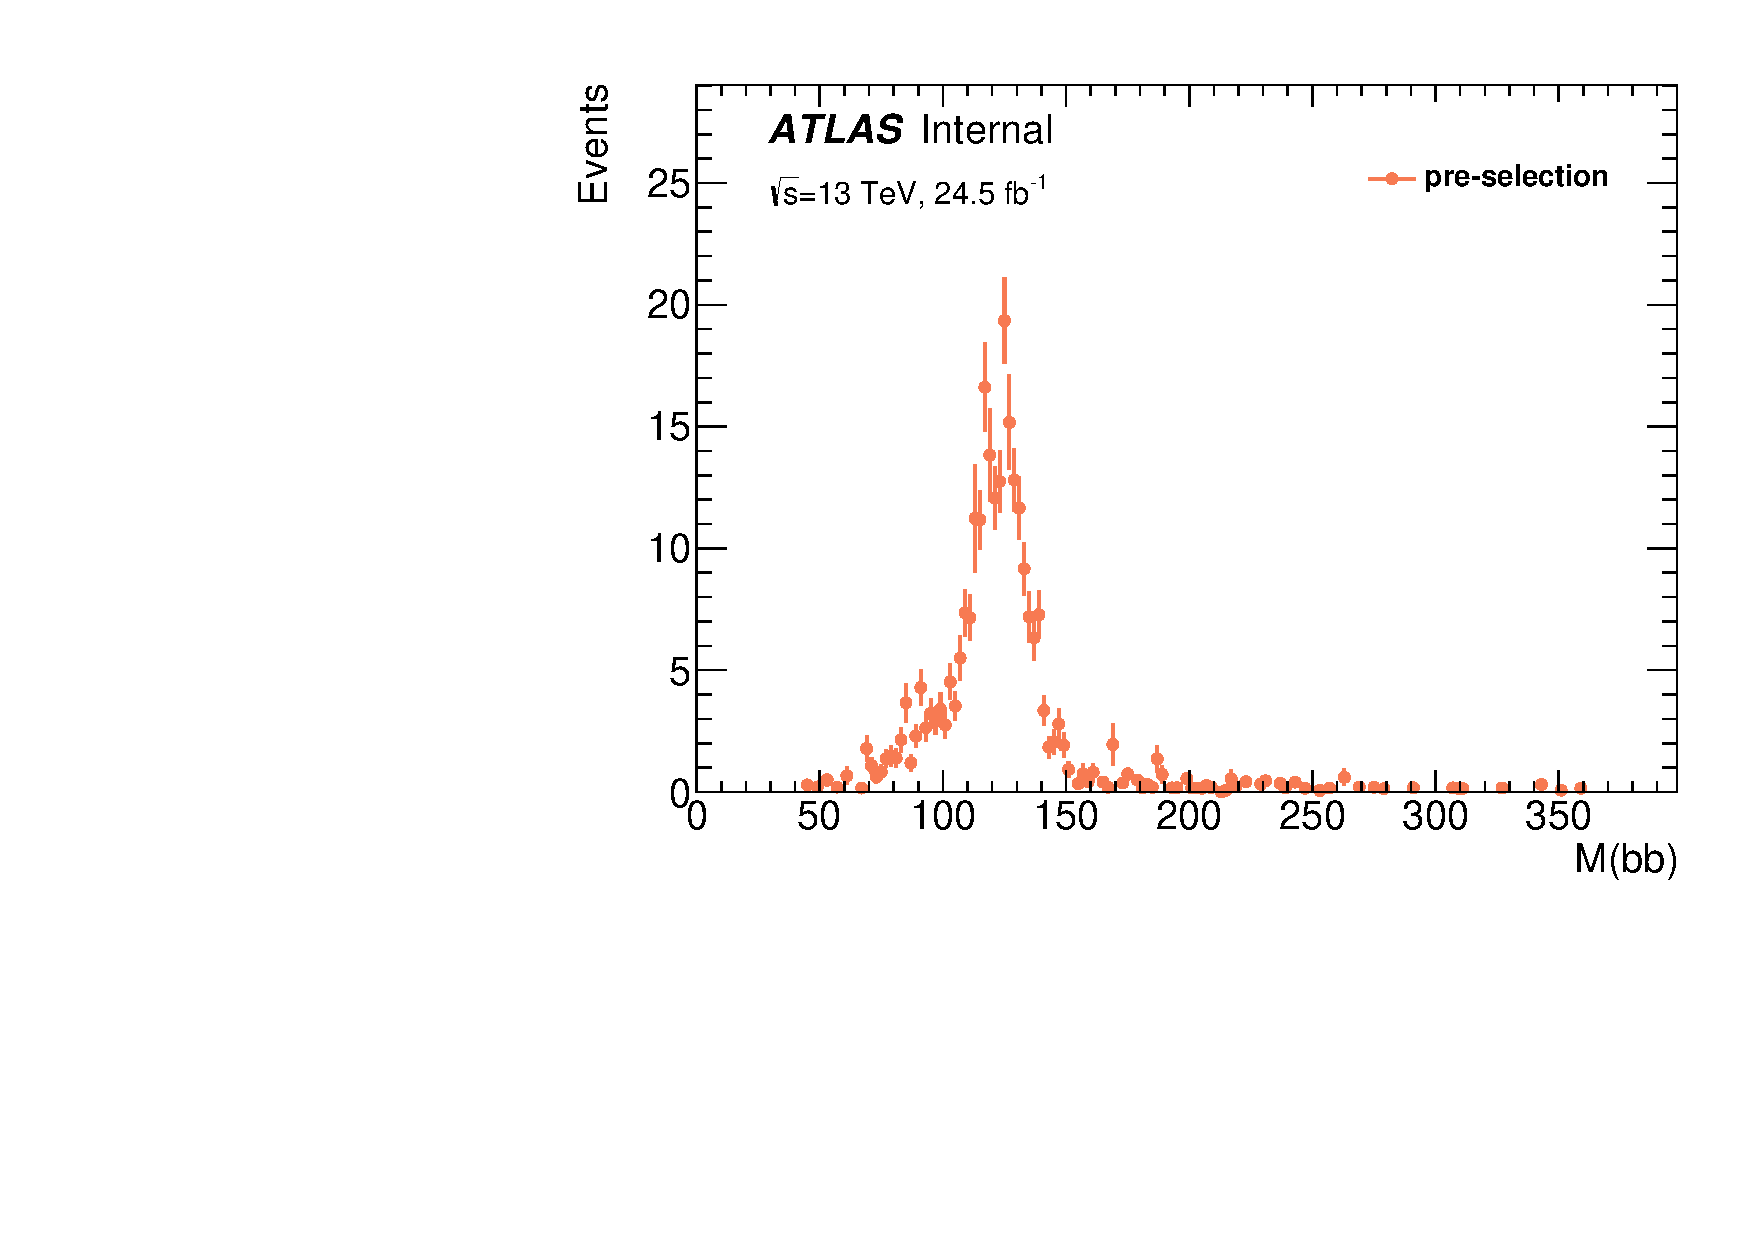
\includegraphics[width=0.42\textwidth]{figures/VBF/Mbb_VH_4cen.pdf}
 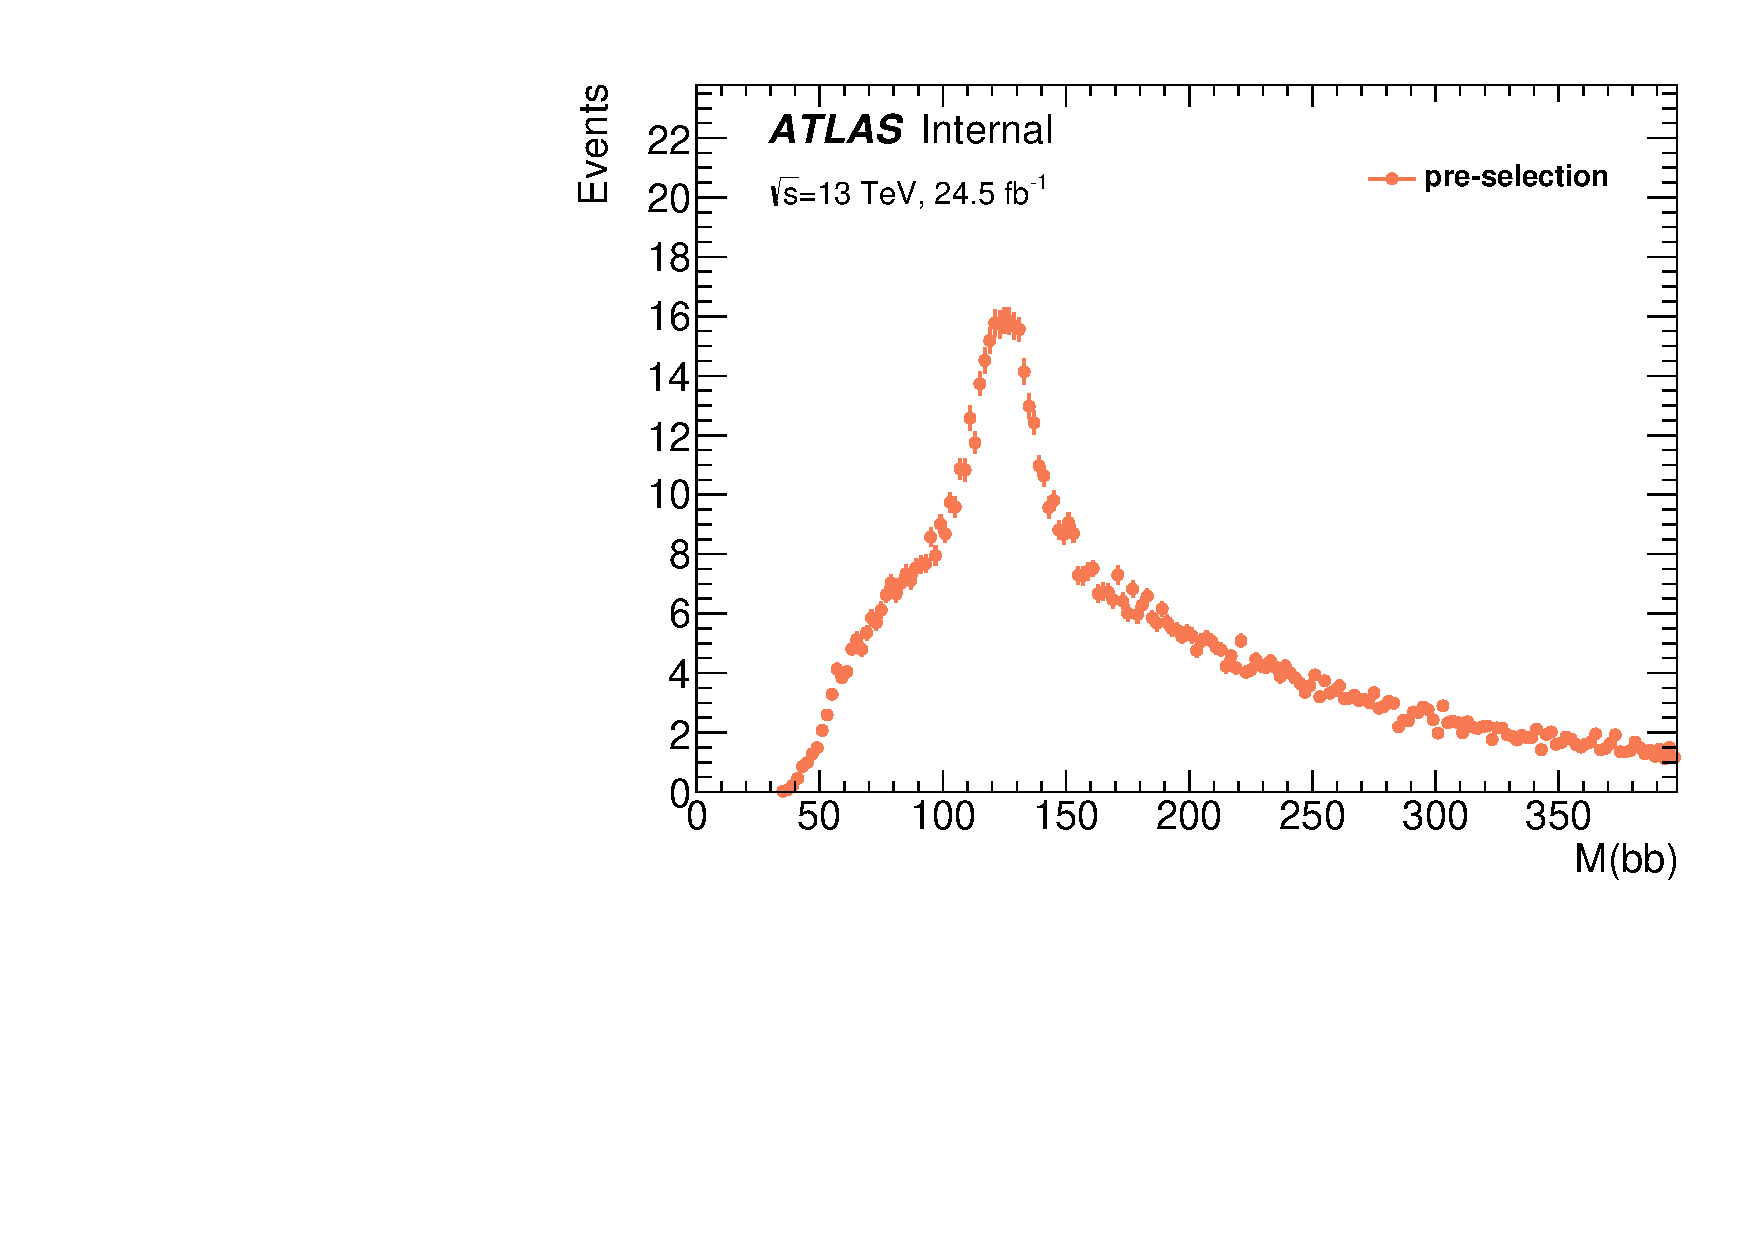
\includegraphics[width=0.42\textwidth]{figures/VBF/Mbb_ttH_4cen.pdf}
 \caption{\Mbb distributions of \VH (left) and \ttH (right) for \twocentral (top) and \fourcentral (bottom) channels passing event pre-selection. }
  \label{fig:Mbb-ttH-VH}
\end{figure}

\begin{table}[htbp]
\centering
\caption{Yields of \VH and \ttH}
\label{tab:vh-tth-yield}
\begin{tabular}{|l|l|l|l|l|}
\hline
     & \multicolumn{2}{l|}{\twocentral SR I}    & \multicolumn{2}{l|}{\twocentral SR II}  \\ \hline
     & Expected Yied  & Fraction of Total Yield & Expected Yied & Fraction of Total Yield \\ \hline
\VH  & 0.2           & 0.2\%                  & 9.3          & 6.8\%                  \\ \hline
\ttH & 4.2           & 2.9\%                  & 30.0         & 19.7\%                 \\ \hline
     & \multicolumn{2}{l|}{\fourcentral SR I}   & \multicolumn{2}{l|}{\fourcentral SR II} \\ \hline
     & Expected Yied  & Fraction of Total Yield & Expected Yied & Fraction of Total Yield \\ \hline
\VH  & 1.4           & 2.0\%                  & 0.7          & 1.4\%                  \\ \hline
\ttH & 0.6           & 0.8\%                  & 2.2          & 4.2\%                  \\ \hline
     & \multicolumn{2}{l|}{\fourcentral SR III} & \multicolumn{2}{l|}{\fourcentral SR IV} \\ \hline
     & Expected Yied  & Fraction of Total Yield & Expected Yied & Fraction of Total Yield \\ \hline
\VH  & 6.0           & 5.2\%                  & 34.1         & 13.5\%                  \\ \hline
\ttH & 12.4          & 10.2\%                 & 42.4         & 15.5\%                 \\ \hline
\end{tabular}
\end{table}

\clearpage

\subsubsection{Summary}
The typical signal yield changes due to a few representative systematic uncertainties are 
shown in Tables. \ref{tab:syst-2cen} and \ref{tab:syst-4cen}.  The theory uncertainties, especially from the QCD scale dominate, at the 20\% level across all signal regions.  The largest experimental uncertainties are from \btagging, at the 3--4\% level.

\begin{table}[hbpt]
\centering
\scriptsize
\begin{tabular}{|l|l|l|l|l|l|l|}
\hline
                 & \multicolumn{6}{c|}{\twocentral}                     \\ \hline
                 & \multicolumn{3}{c|}{SRI} & \multicolumn{3}{c|}{SRII} \\ \hline
                 & Total  & VBF    & ggF    & Total   & VBF    & ggF    \\ \hline
Jet Energy Scale NP1           & 0.75   & 1.19   & 1.14   & 2.54    & 4.11   & 2.07   \\ \hline
Jet Energy Scale \bjets        & 1.52   & 1.62   & 1.08   & 2.21    & 2.71   & 2.06   \\ \hline
Jet Energy Resolution          & 1.65   & 3.03   & 4.11   & 2.16    & 4.69   & 4.19   \\ \hline
\qgtagging                     & 0.65   & 0.73   & 0.28   & 1.39    & 2.12   & 1.18   \\ \hline
Pile-up Reweighting            & 0.49   & 0.18   & 1.74   & 0.18    & 0.99   & 0.54   \\ \hline
\btagging NP0 70WP             & 2.66   & 2.67   & 2.60   & 2.88    & 2.74   & 2.92   \\ \hline
\btagging NP0 85WP             & 0.80   & 0.87   & 0.52   & 1.26    & 1.08   & 1.31   \\ \hline
$\alpha_s$                     & 0.73   & 0.14   & 3.18   & 2.66    & 3.95   & 3.35   \\ \hline
QCD scale VBF                  & 9.92   & 12.29  & 0      & 2.41    & 10.50  & 0      \\ \hline
QCD scale ggF                  & 8.17   & 0      & 42.33  & 29.61   & 0      & 41.91  \\ \hline
PDF Variations                 & 10.08  & 11.52  & 4.16   & 6.36    & 9.56   & 5.42   \\ \hline
Parton Shower                  & 0.34   & 1.06   & 2.69   & 0.62    & 1.92   & 0.24   \\ \hline
\end{tabular}
\caption{Yield change in percentage due to $\pm 1 \sigma$ variation of systematics for \twocentral for combined signal, VBF and ggF production modes. }
\label{tab:syst-2cen}
\end{table}


\begin{table}[hbpt]
\centering
\scriptsize
\begin{tabular}{|l|l|l|l|l|l|l|l|l|l|l|l|l|}
\hline
                    & \multicolumn{12}{c|}{\fourcentral}                                                                                \\ \hline
                    & \multicolumn{3}{c|}{SR I} & \multicolumn{3}{c|}{SR II} & \multicolumn{3}{c|}{SR III} & \multicolumn{3}{c|}{SR IV} \\ \hline
                    & Total   & VBF    & ggF    & Total   & VBF     & ggF    & Total   & VBF     & ggF     & Total   & VBF     & ggF    \\ \hline
Jet Energy Scale NP1      & 3.38    & 1.05   & 18.50  & 0.65    & 0.57    & 3.10   & 1.56    & 2.43    & 0.76    & 1.12    & 0.59    & 1.44   \\ \hline
Jet Energy Scale \bjets   & 0.21    & 0.64   & 1.67   & 1.48    & 1.57    & 12.9   & 0.49    & 1.35    & 0.31    & 1.66    & 2.25    & 1.46   \\ \hline
Jet Energy Resolution     & 1.16    & 1.25   & 12.04  & 0.35    & 2.20    & 3.38   & 3.96    & 1.14    & 8.64    & 1.13    & 0.79    & 1.78   \\ \hline
\qgtagging                & 3.98    & 2.41   & 10.69  & 0.21    & 0.60    & 1.86   & 0.33    & 1.81    & 0.22    & 0.11    & 4.27    & 1.56   \\ \hline
Pile-up Reweighting       & 0.34    & 0.38   & 0.17   & 2.17    & 2.06    & 4.19   & 1.49    & 0.19    & 3.04    & 2.55    & 2.23    & 2.66   \\ \hline
\btagging NP0 77WP        & 4.37    & 4.33   & 4.53   & 4.19    & 4.17    & 4.23   & 4.30    & 4.12    & 4.47    & 4.21    & 4.15    & 4.25   \\ \hline
$\alpha_s$                & 0.76    & 0.16   & 3.35   & 1.32    & 0.23    & 3.45   & 1.85    & 0.34    & 3.23    & 2.85    & 0.90    & 3.49   \\ \hline
QCD scale VBF             & 6.69    & 8.25   & 0      & 5.39    & 8.06    & 0      & 3.86    & 8.08    & 0       & 1.98    & 7.95    & 0      \\ \hline
QCD scale ggF             & 7.83    & 0      & 41.56  & 12.86   & 0       & 40.66  & 22.67   & 0       & 43.42   & 31.99   & 0       & 42.60  \\ \hline
PDF Variations            & 6.19    & 6.44   & 5.16   & 5.62    & 6.33    & 4.18   & 5.03    & 6.11    & 4.05    & 4.95    & 7.23    & 4.19   \\ \hline
Parton Shower             & 3.24    & 4.14   & 0.62   & 1.75    & 3.56    & 1.87   & 2.36    & 0.31    & 0.96    & 0.26    & 0.32    & 0.24   \\ \hline
\end{tabular}
\caption{Yield change in percentage due to $\pm 1 \sigma$ variation of systematics for \fourcentral for combined signal, VBF and ggF production modes.}
\label{tab:syst-4cen}

\end{table}




\subsection{Profile Likelihood and yield determination}

The negative log-likelihood is constructed as shown in Eq.\ref{likelihood}, 
where $Y_{ijk}$ denotes the yield of $k^{th}$ bin of $j^{th}$ region of $i^{th}$ channel. 
Nuisance parameters, which have external constraints $f(\alpha_l)$, are penalized in the negative log-likelihood. 
b
Both \twocentral{} and  \fourcentral{} channel consists of four signal regions and yield in total eight \Mbb{} distributions.
The yield of a given region R is calculated with Eq.\ref{yield_float}. Note in the equation that a Gaussian constraint $\alpha_{sp}$ 
for spurious signal is included with width being the spurious signal size we measured in the spurious signal test.

Free parameters are the normalizations of the non-resonant background in each control and
signal region, denoted with $N_B$.
The signal normalizations $N_H$ are set to the Standard Model expectation from simulation,
while $\mu$ represents the observed signal strength.
The shapes of Higgs, Z and non-resonant background are $H$, $Z$ and $B$, respectively.

\begin{equation}
\label{likelihood}
-\log\mathcal{L}(\mu, \{\alpha_{l}\} )= -\log \prod_{i=1}^{\textnormal{Channels}} \prod_{j=1}^{\textnormal{Regions}} \prod_{k=1}^{\textnormal{Bins}} \frac{e^{-Y_{ijk}(\mu, \{\alpha_l\})} \times Y_{ijk}N_{ijk}^{Obs} }{N_{ijk}^{Obs}} - \log \prod_{l}^{\textnormal{Nuisance Pars}} f(\alpha_l)
\end{equation}

\begin{equation}
\label{yield_float}
\begin{split}
Y(R) &= (\mu + \alpha_{sp}(R))N_{H}H(R)+ N_{B}B(R)+ \mu_{z}(R)N_{Z}Z  \\
\end{split}
\end{equation}


The Eq.\ref{yield_float} adopts the strategy floating the $Z$ contributions in all BDT regions. In case we adopt the method only floating the $Z$ contributions in SR I and SR II of \twocentral, the rest of the regions will have yield as in Eq.\ref{yield_constrain} where $\mu_z(Norm)$ stands for the floating parameters for $Z$ normalization and $\alpha_z(R)$ stands for the BDT shape nuisance parameter with 50\% width. 

\begin{equation}
\label{yield_constrain}
\begin{split}
Y(R) &= (\mu + \alpha_{sp}(R))N_{H}H(R)+ N_{B}B(R)+ \mu_{z}(Norm)\alpha_z(R)N_{Z}Z  \\
\end{split}
\end{equation}



%The nuisance parameter $\alpha_{z}$ controls the overall normalization for the \zjets{} template 
%and is constrained with a Gaussian prior with width 0.06. The overall normalization is scaled
% to 0.81 and 0.75 for \twocentral and \fourcentral channels, respectively, determined as described in Section~\ref{sec:ztreat}..
%We also adopt independent NPs for each BDT region to account the data/MC shape difference of \zjets{}. 
%The chosen values are motivated by the validation study in data described in Appendix~\ref{sec:zjets}. 


\subsubsection{Fit toy experiments}

To determine if the fit procedure yields bias, we build 1000 toy experiments from the background function determined in background only fit and inject the \Zjets{} component fixed at the Standard Model prediction. The Higgs signals are injected of different strengths at $\mu_{inj} = 0.5, 1.0, 2.0, 5.0$. The pulls of the toy experiment fits defined as $(\mu_{fit}-\mu_{inj})/ \sigma$ are shown in Figures \ref{fig:MCToy}. The distributions of pulls are fitted with Gaussian distribution to determine means and widths, which are consistent with 0 and 1 within statistical uncertainties. For $\mu_{inj}=1.0$ test, as shown in Figures~\ref{fig:2cenAsimov} and~~\ref{fig:4cenAsimov}, we fit back $\hat{\mu}=1.00\pm 1.40$. The expected signal significance in this case is 0.71. (If we adopt the strategy to only float the $Z$ contribution in SR I and SR II of \twocentral channel, we get $\hat{\mu}=1.00\pm 1.35$) The uncertainties and pulls in the fit are shown in Figure~\ref{fig:pull_asimov} and the correlation matrix is shown in Figure~\ref{fig:corr_asimov}


\begin{figure}[htbp]
  \centering
 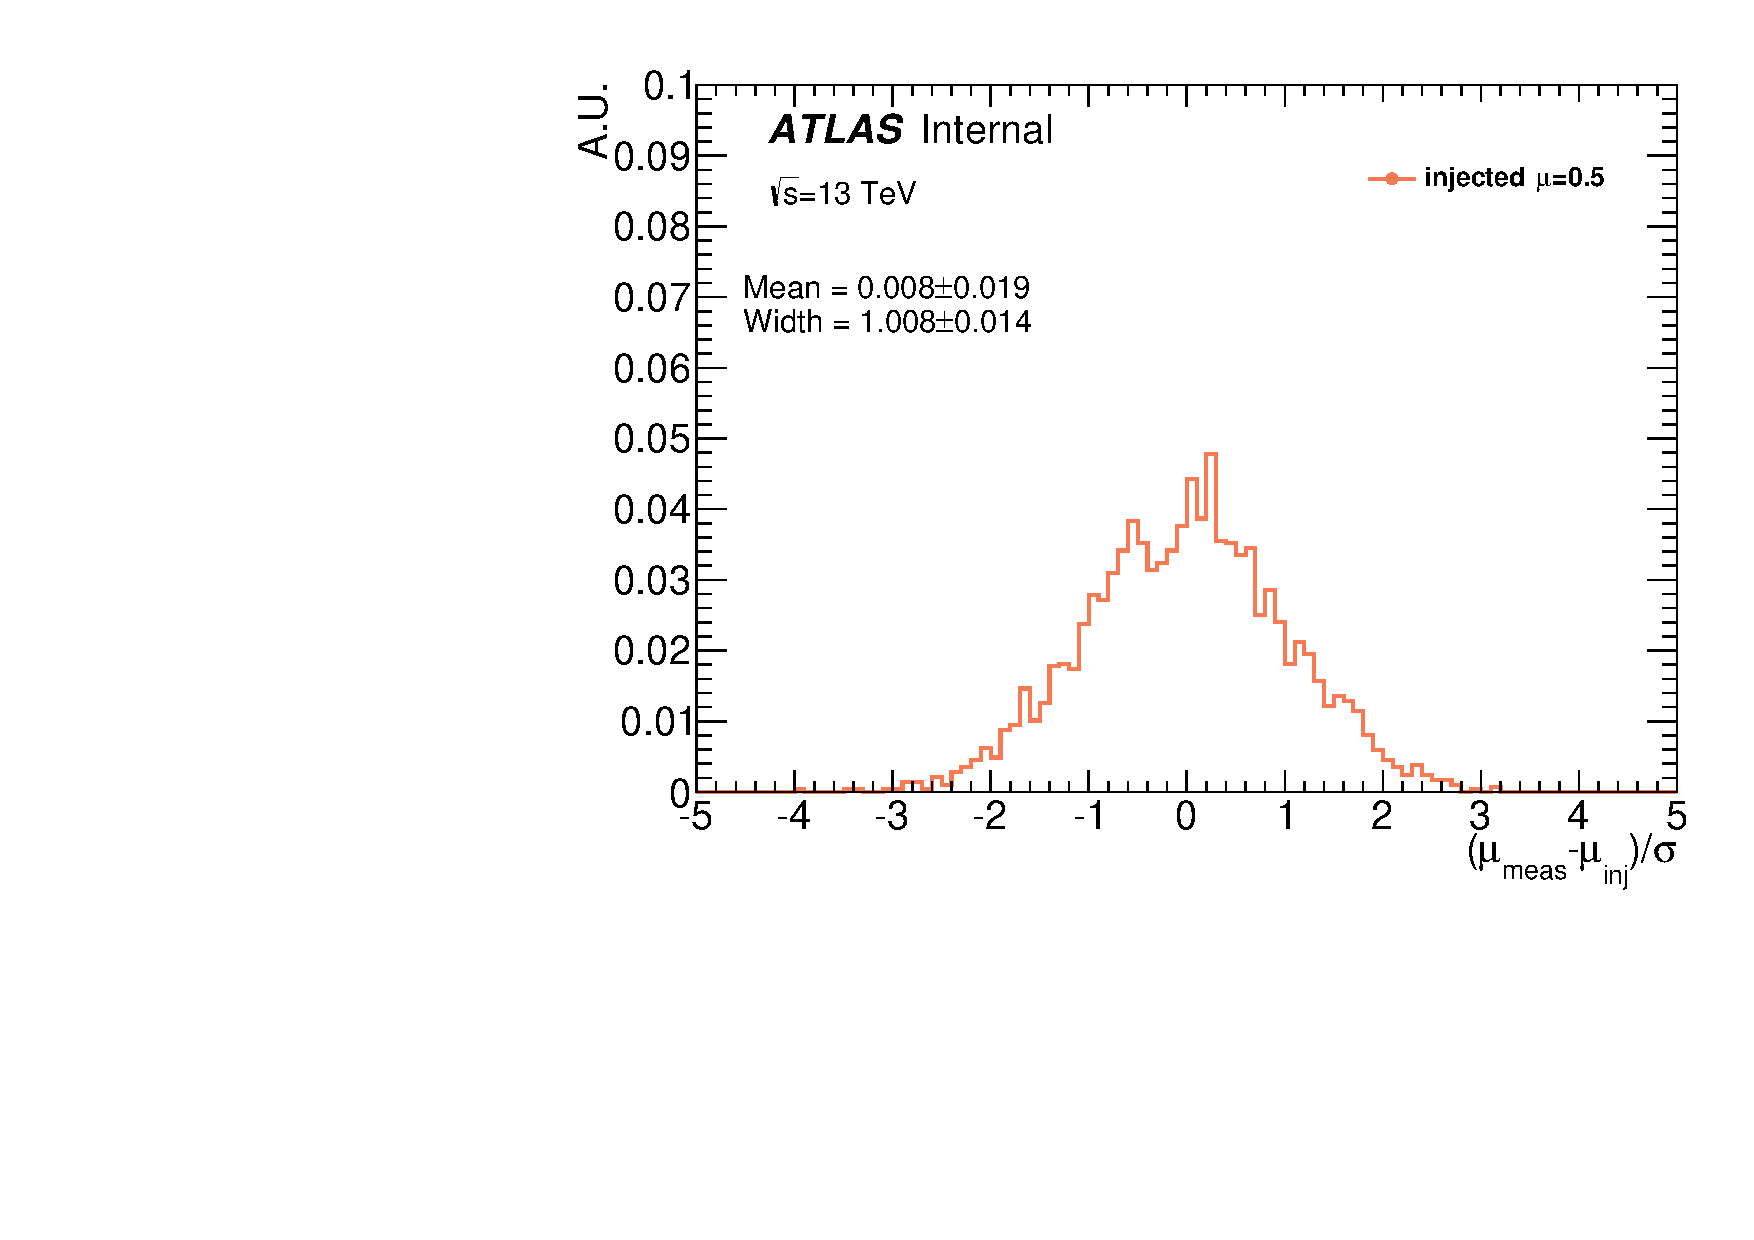
\includegraphics[width=0.45\textwidth]{figures_alt/Mu05.pdf}
 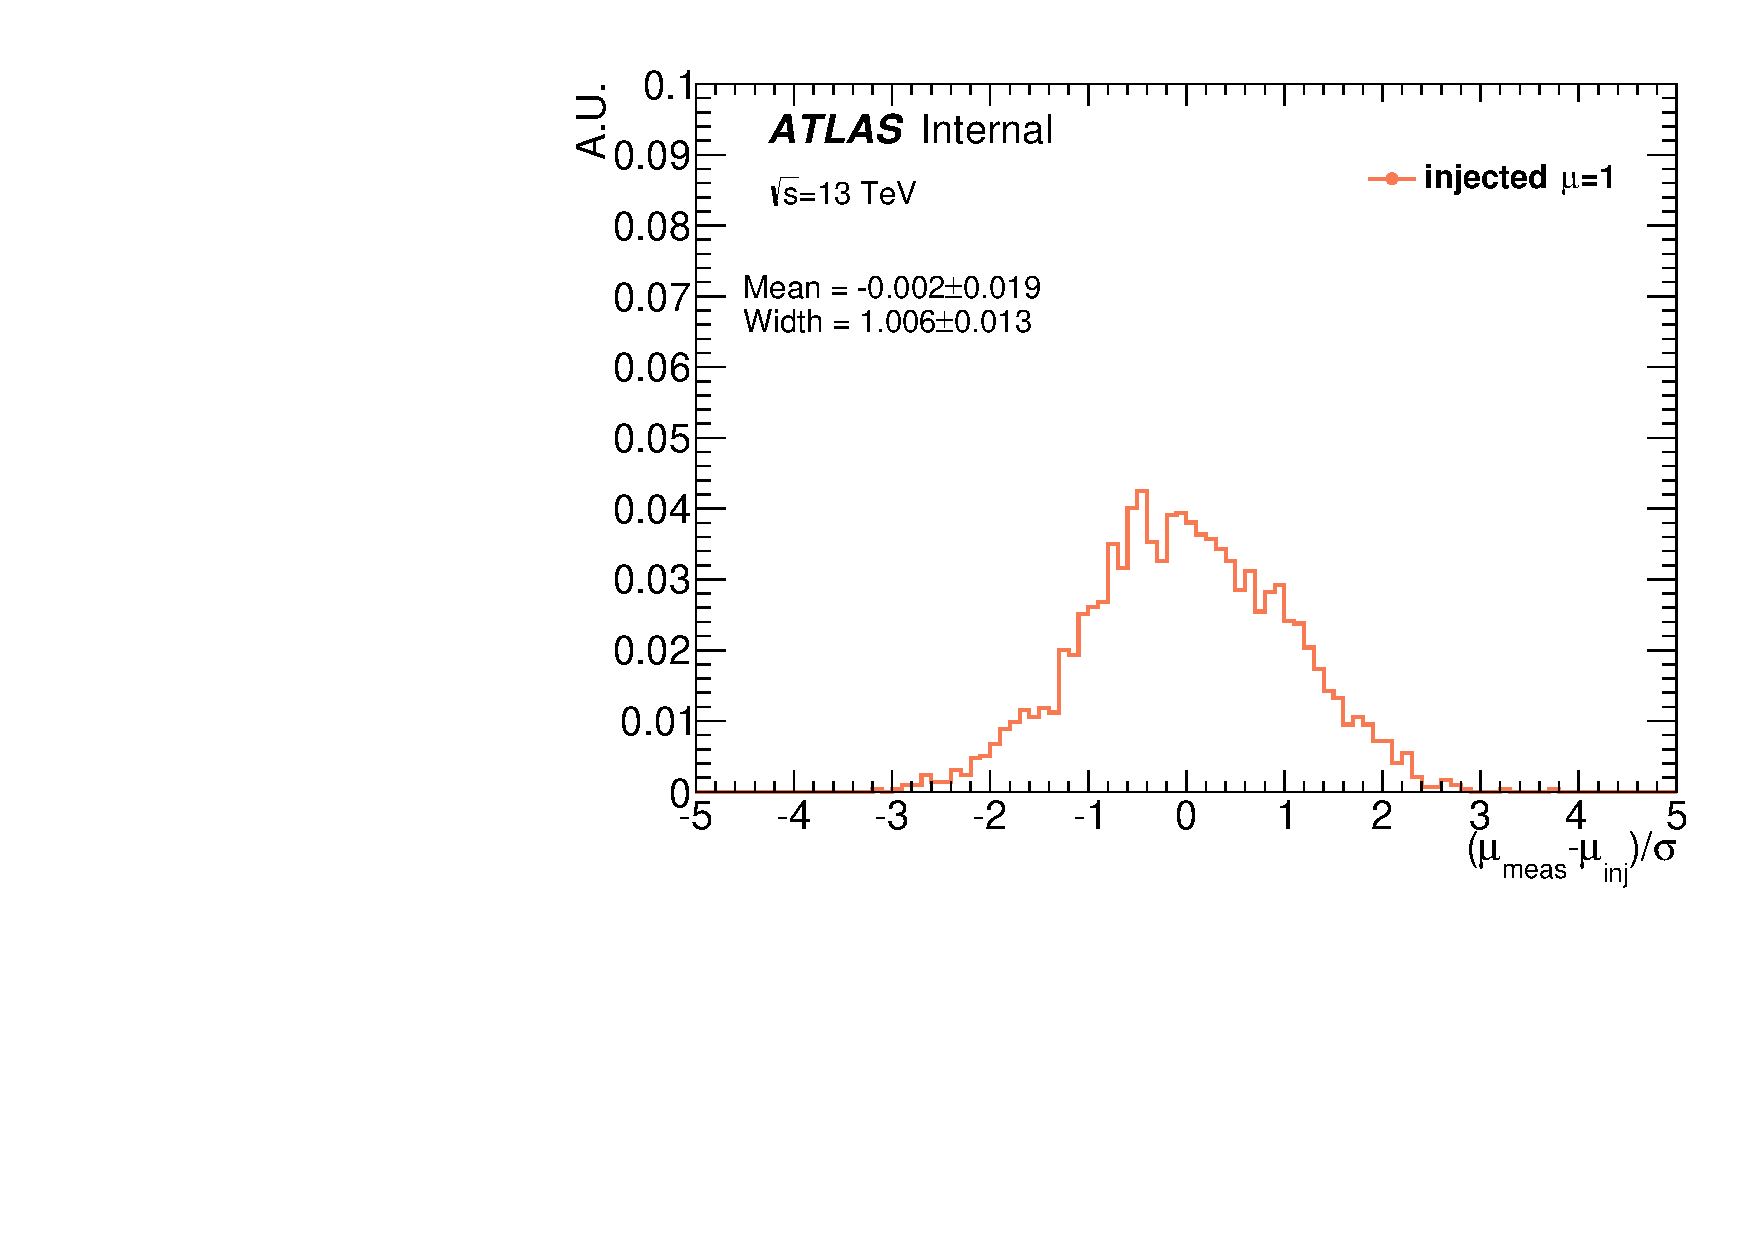
\includegraphics[width=0.45\textwidth]{figures_alt/Mu1.pdf}\\
 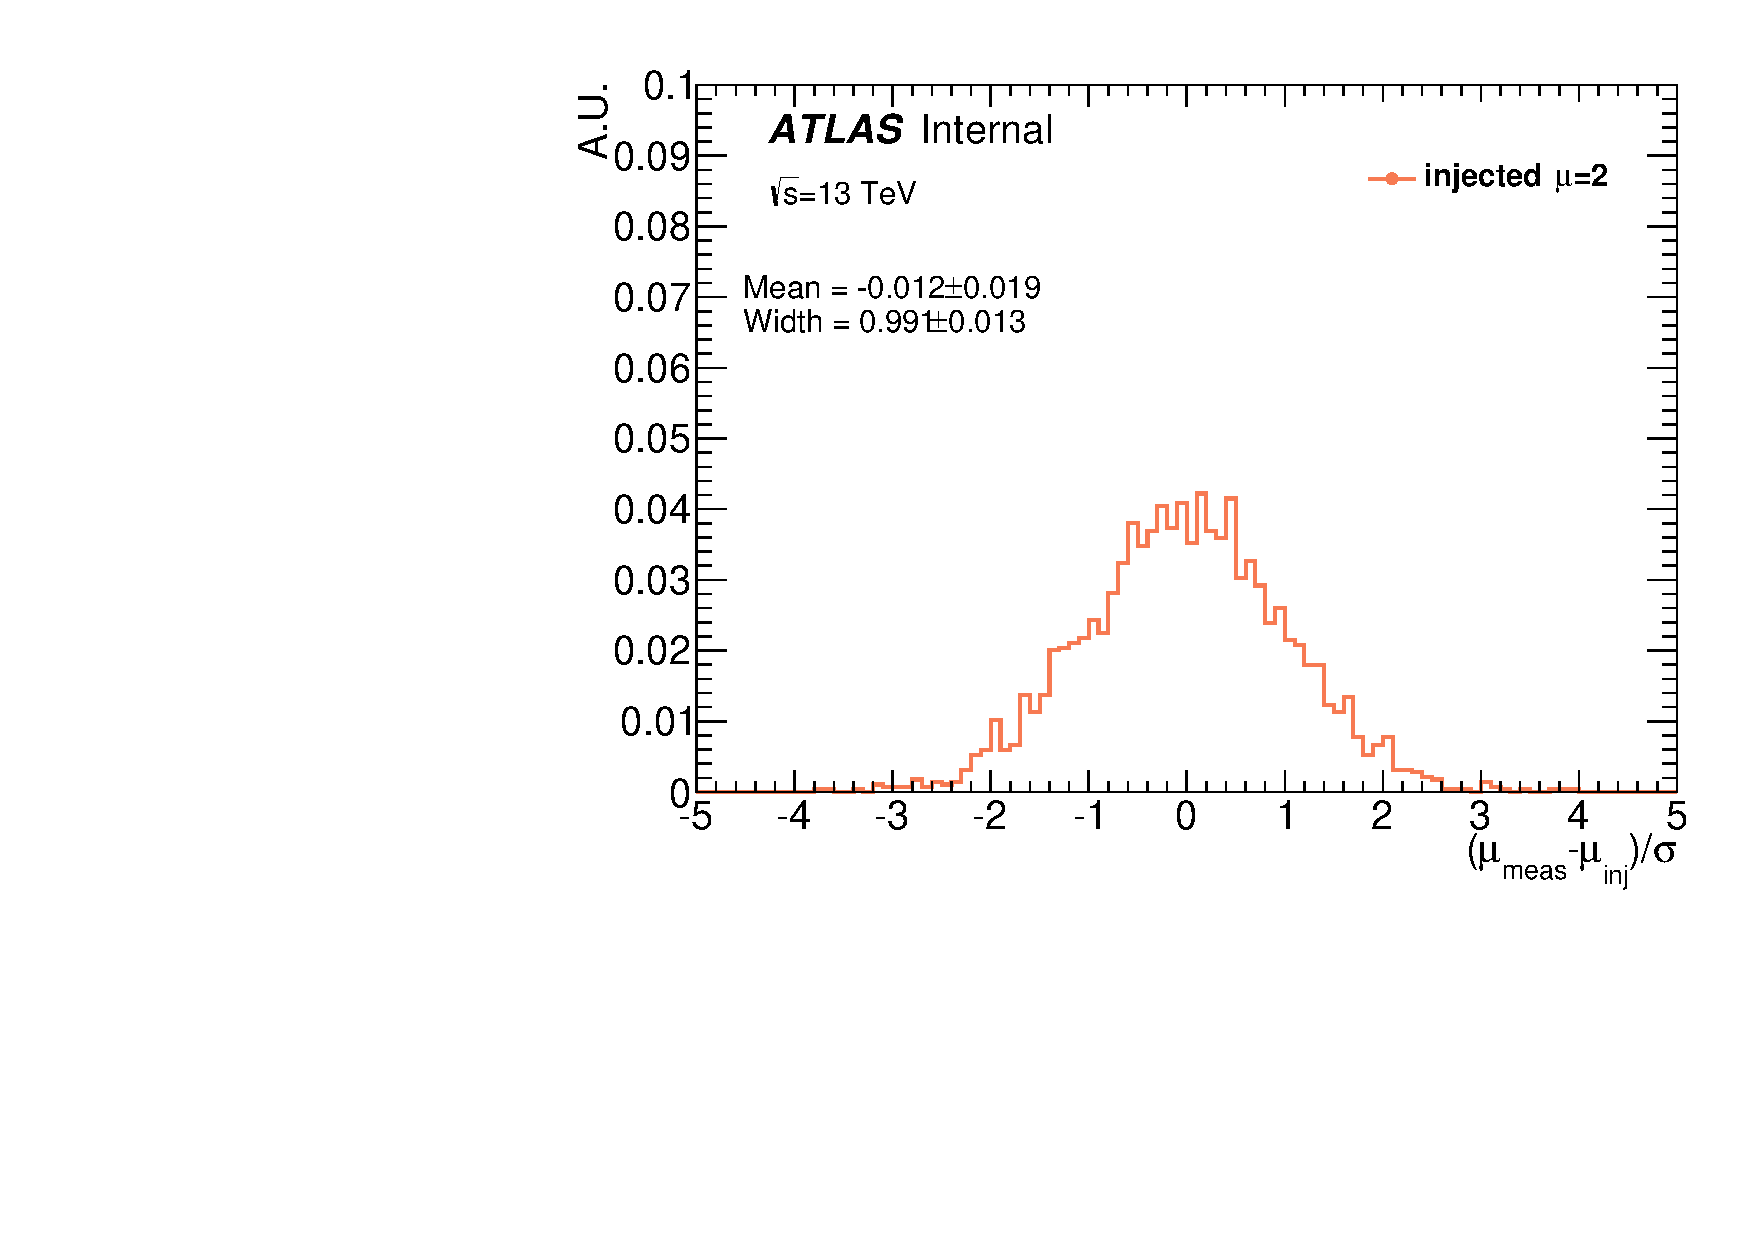
\includegraphics[width=0.45\textwidth]{figures_alt/Mu2.pdf}
 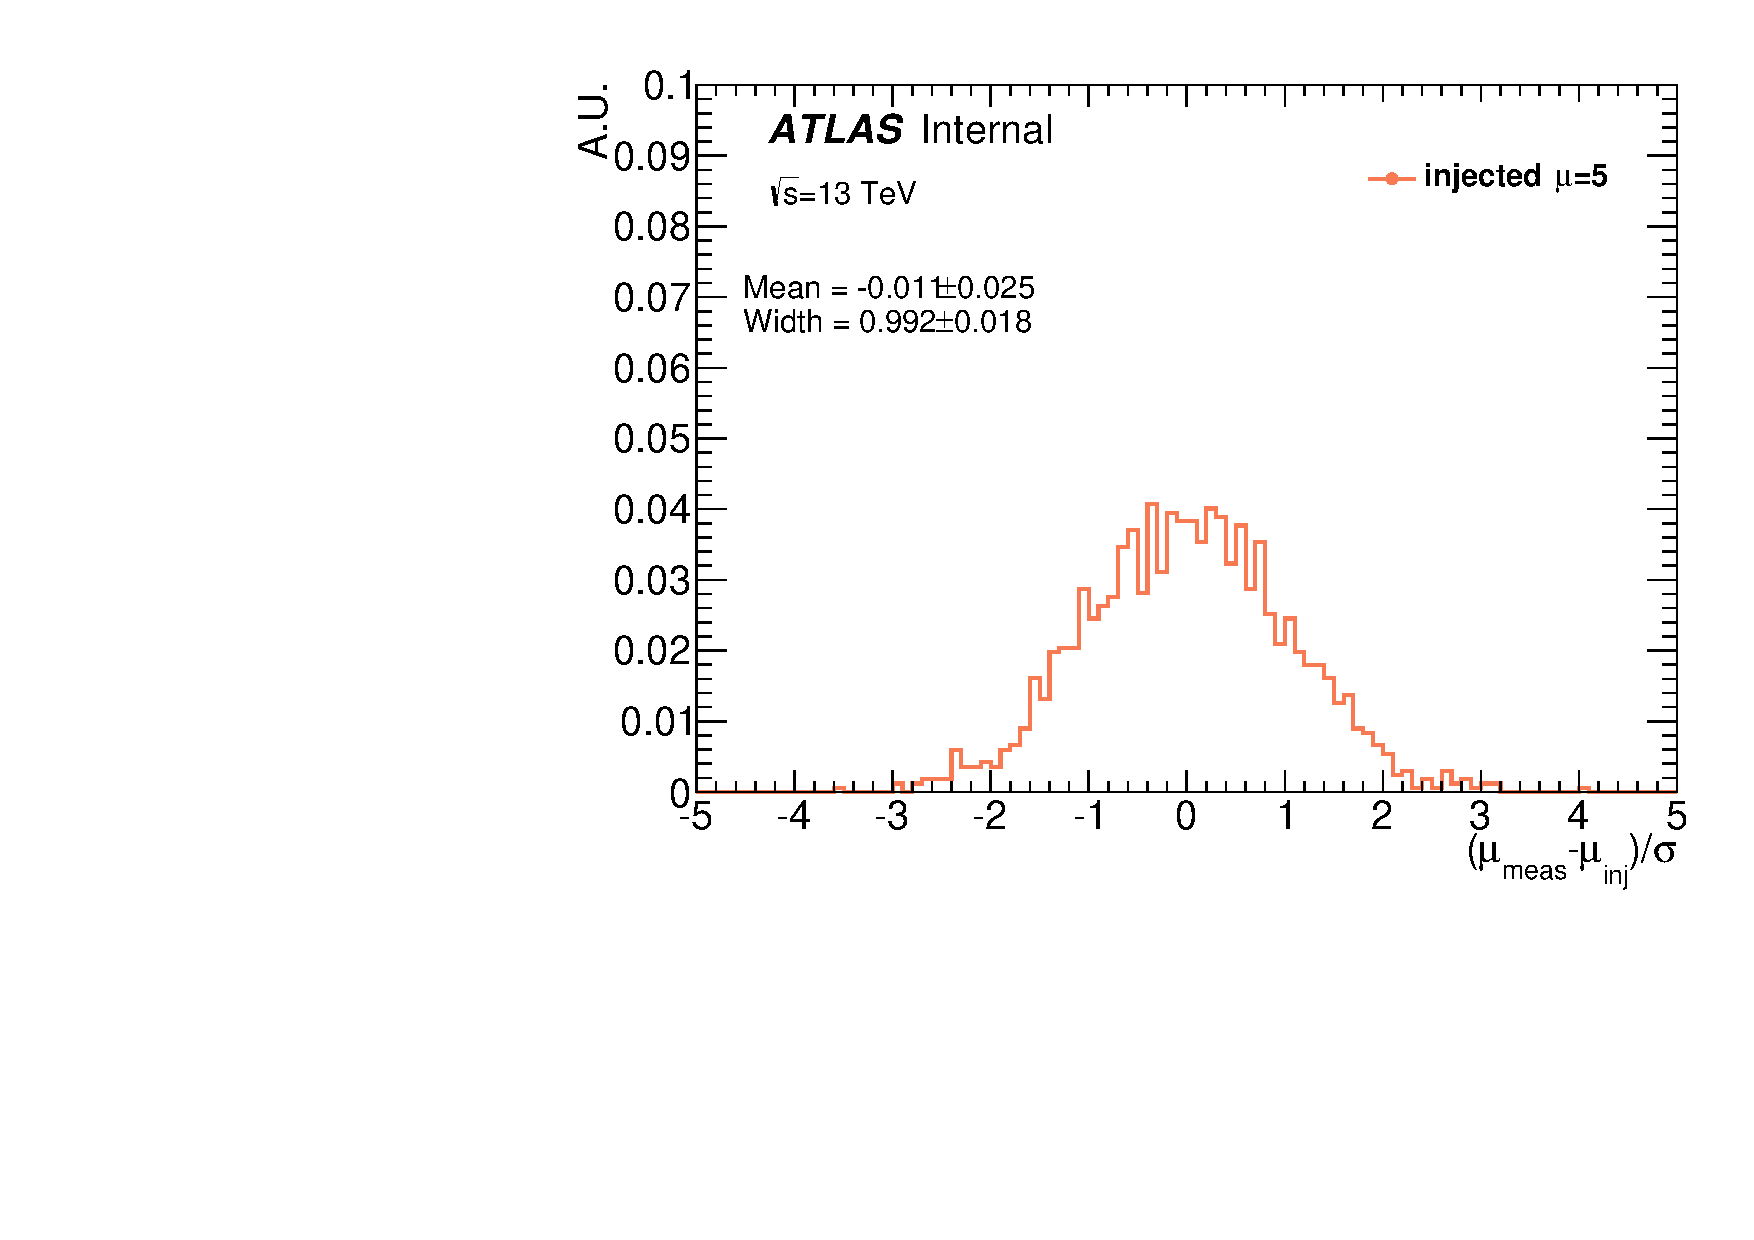
\includegraphics[width=0.45\textwidth]{figures_alt/Mu5.pdf}\\
\caption{Pull distribution of toy experiment fits. We inject Higgs signal strength of 0.5 (top left), 1.0 (top right), 2.0 (bottom left) and 5.0 (bottom right) times the Standard Model prediction. The pulls are fitted with Gaussian to determine the means and widths which are unbiased. }
  \label{fig:MCToy}
\end{figure}


\begin{figure}[htbp]
  \centering
 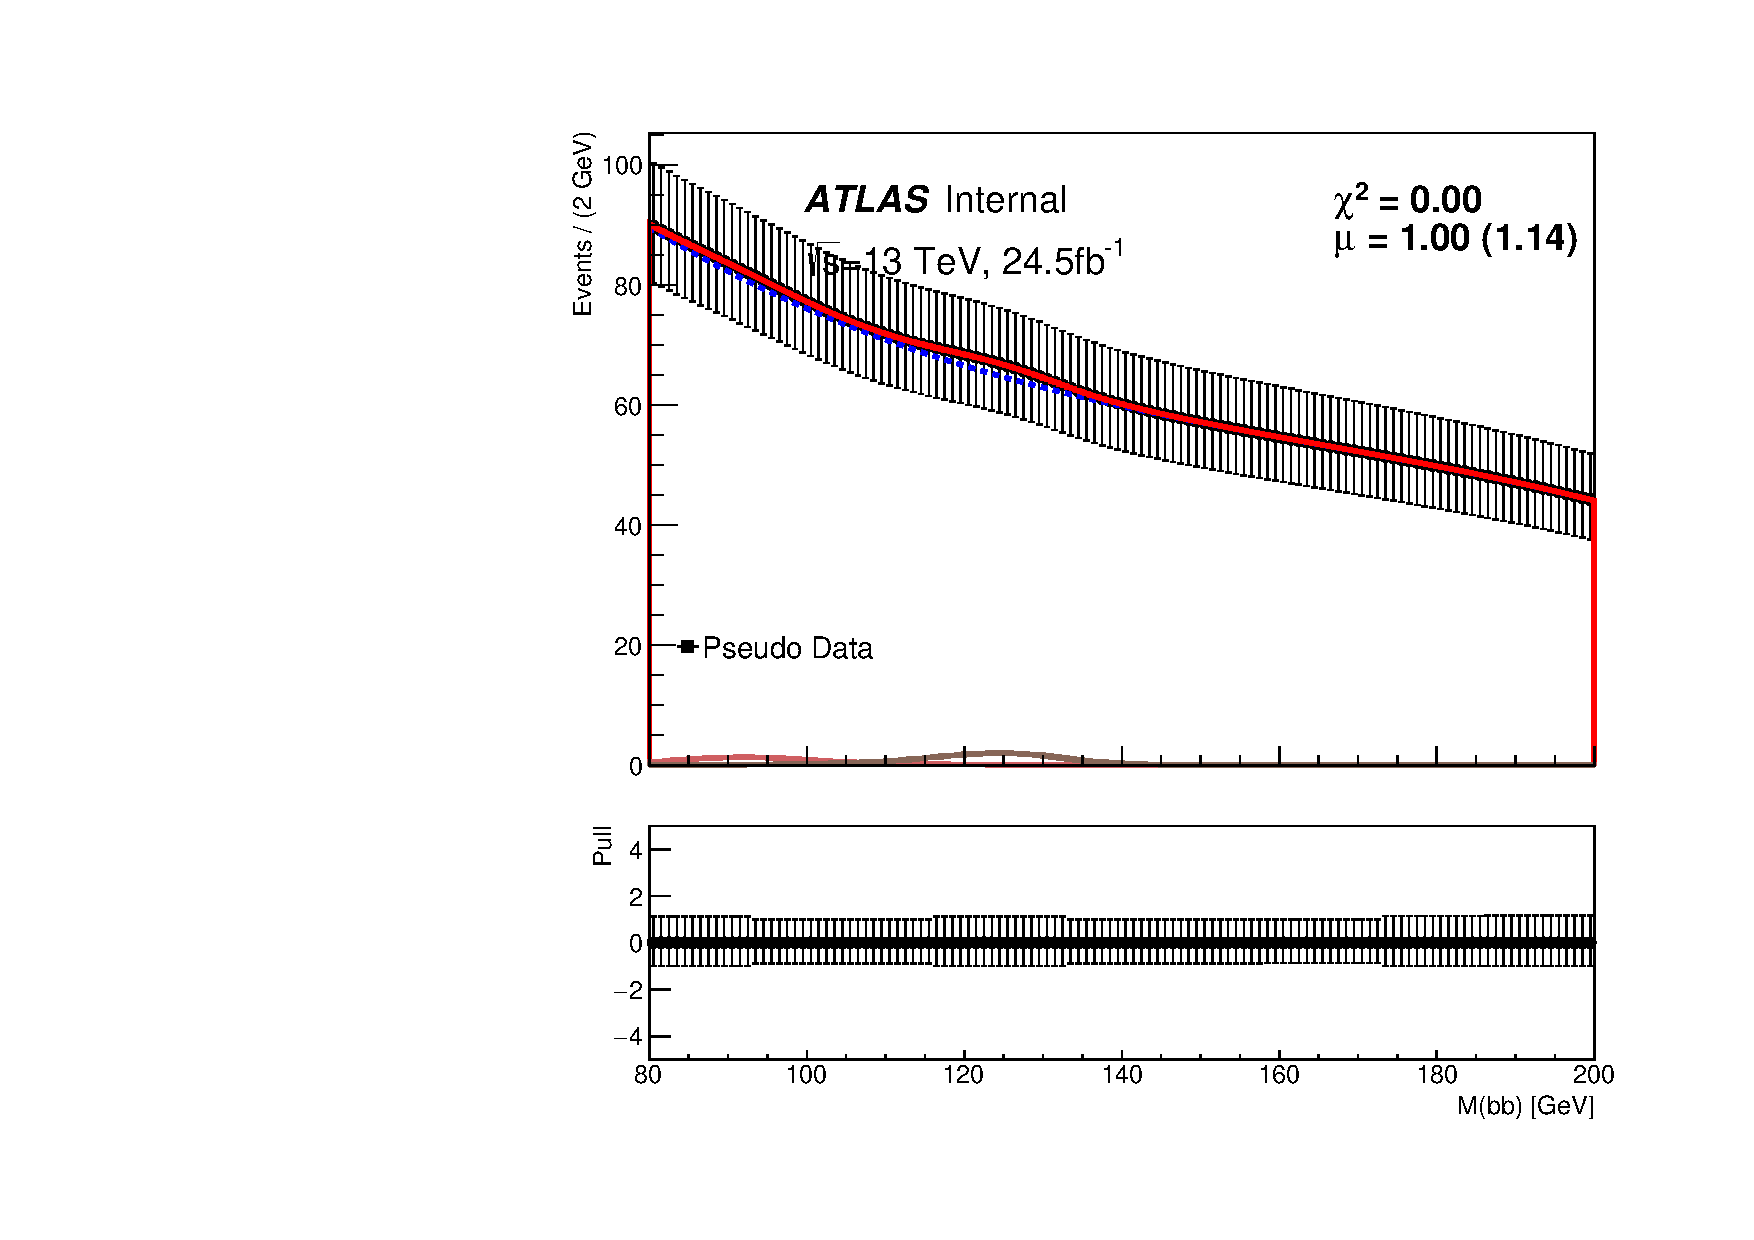
\includegraphics[width=0.48\textwidth]{figures_alt/Asimov_testVBF_ICHEP_2cen_SRI.pdf}
 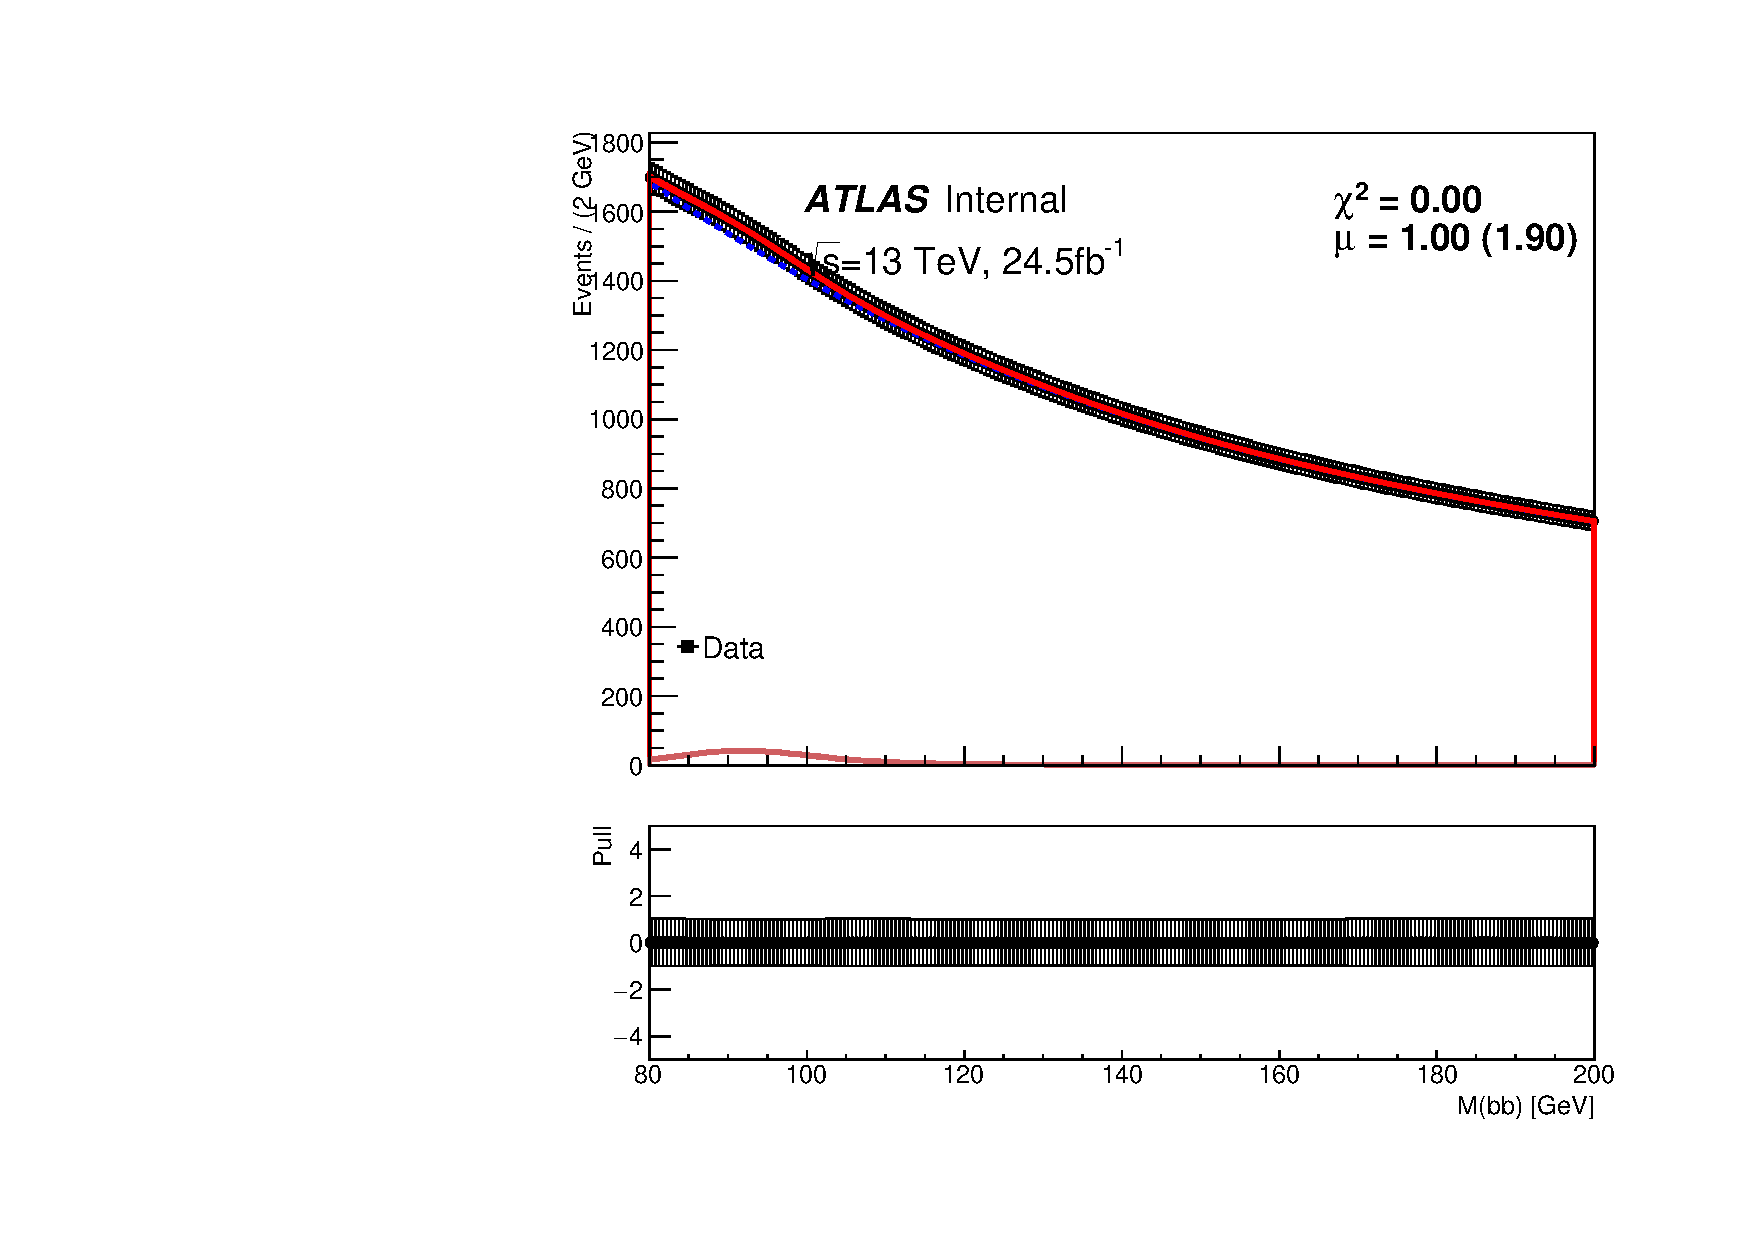
\includegraphics[width=0.48\textwidth]{figures_alt/Asimov_testVBF_ICHEP_2cen_SRII.pdf}
 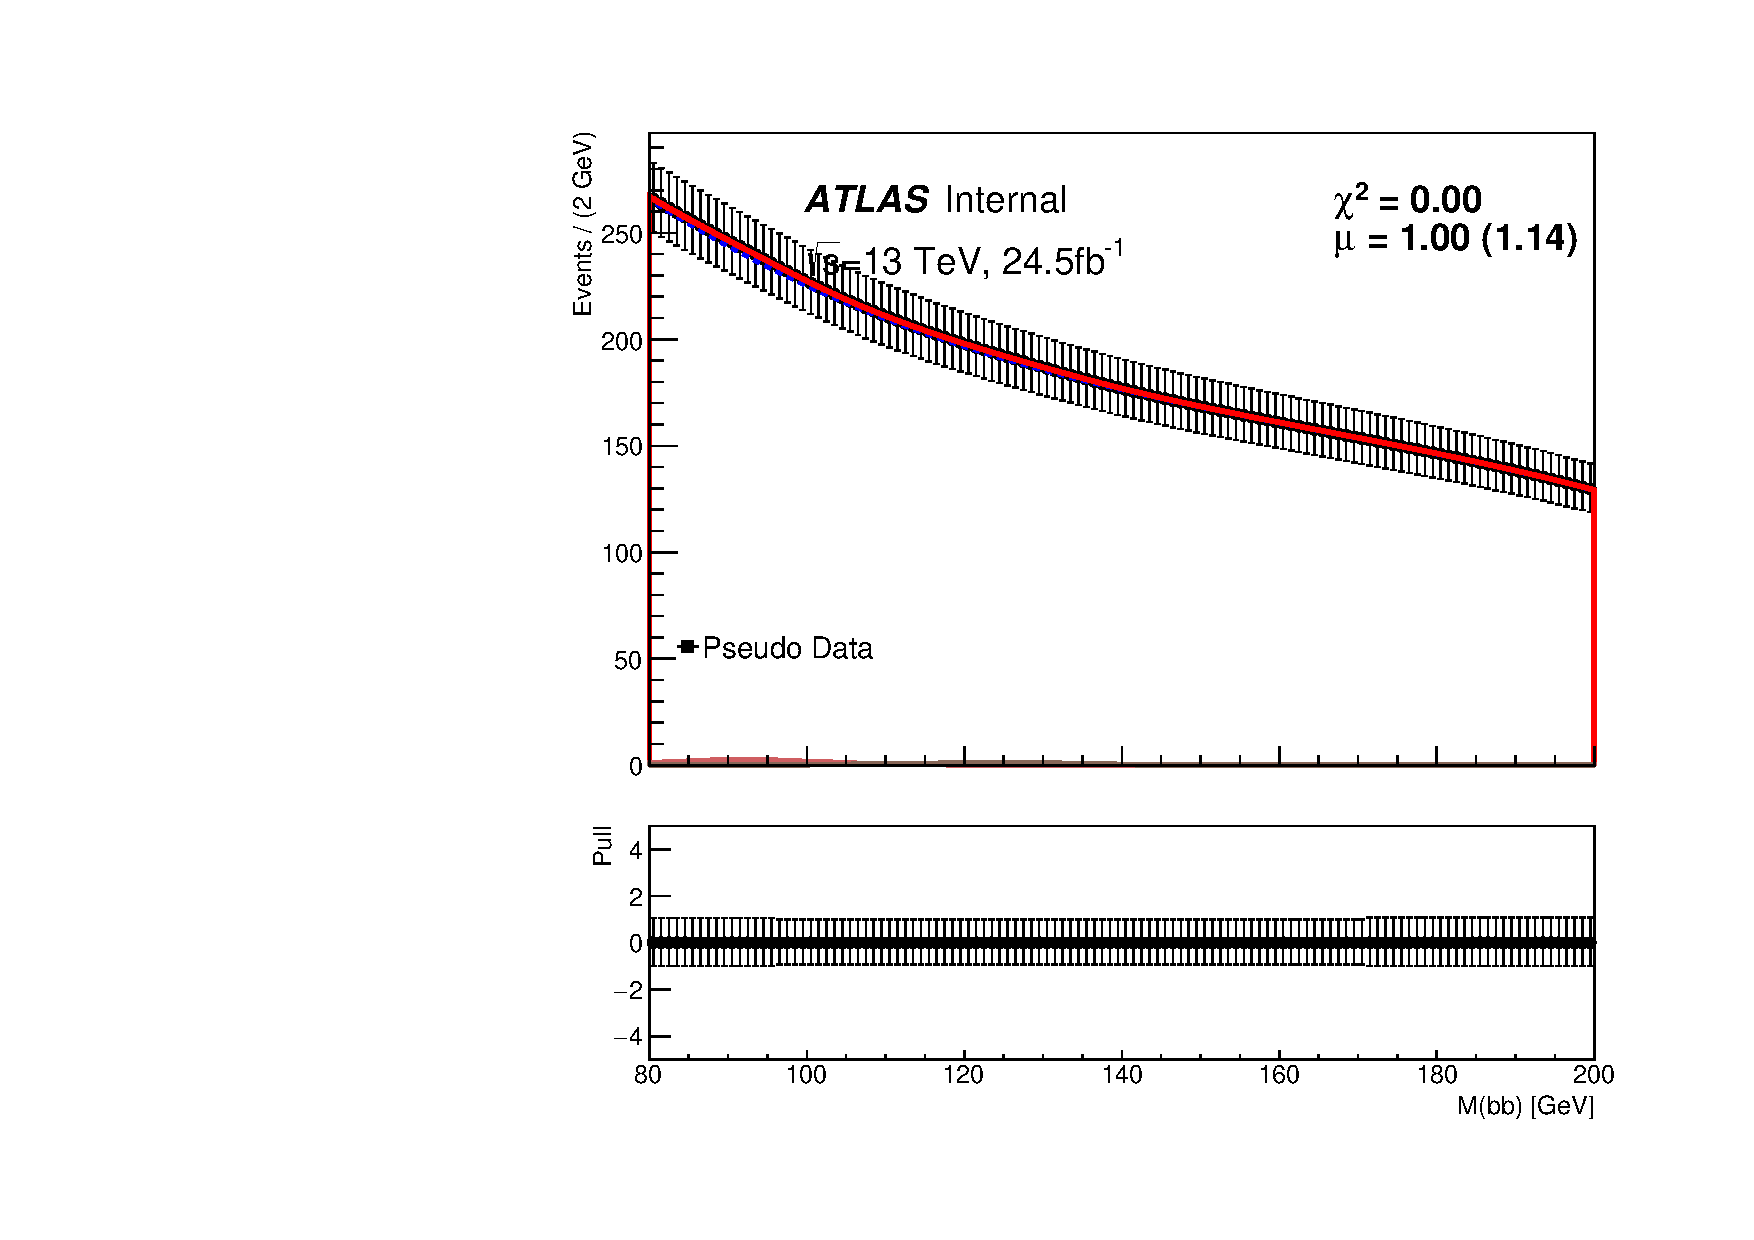
\includegraphics[width=0.48\textwidth]{figures_alt/Asimov_testVBF_ICHEP_2cen_SRIII.pdf}
 \includegraphics[width=0.48\textwidth]{figures_alt/Asimov_testVBF_ICHEP_2cen_SRIV.pdf}\\
\caption{Asymptotic Asimov fits for SR1 to SRIV for the \twocentral channel.}
  \label{fig:2cenAsimov}
\end{figure}

\begin{figure}[htbp]
  \centering
 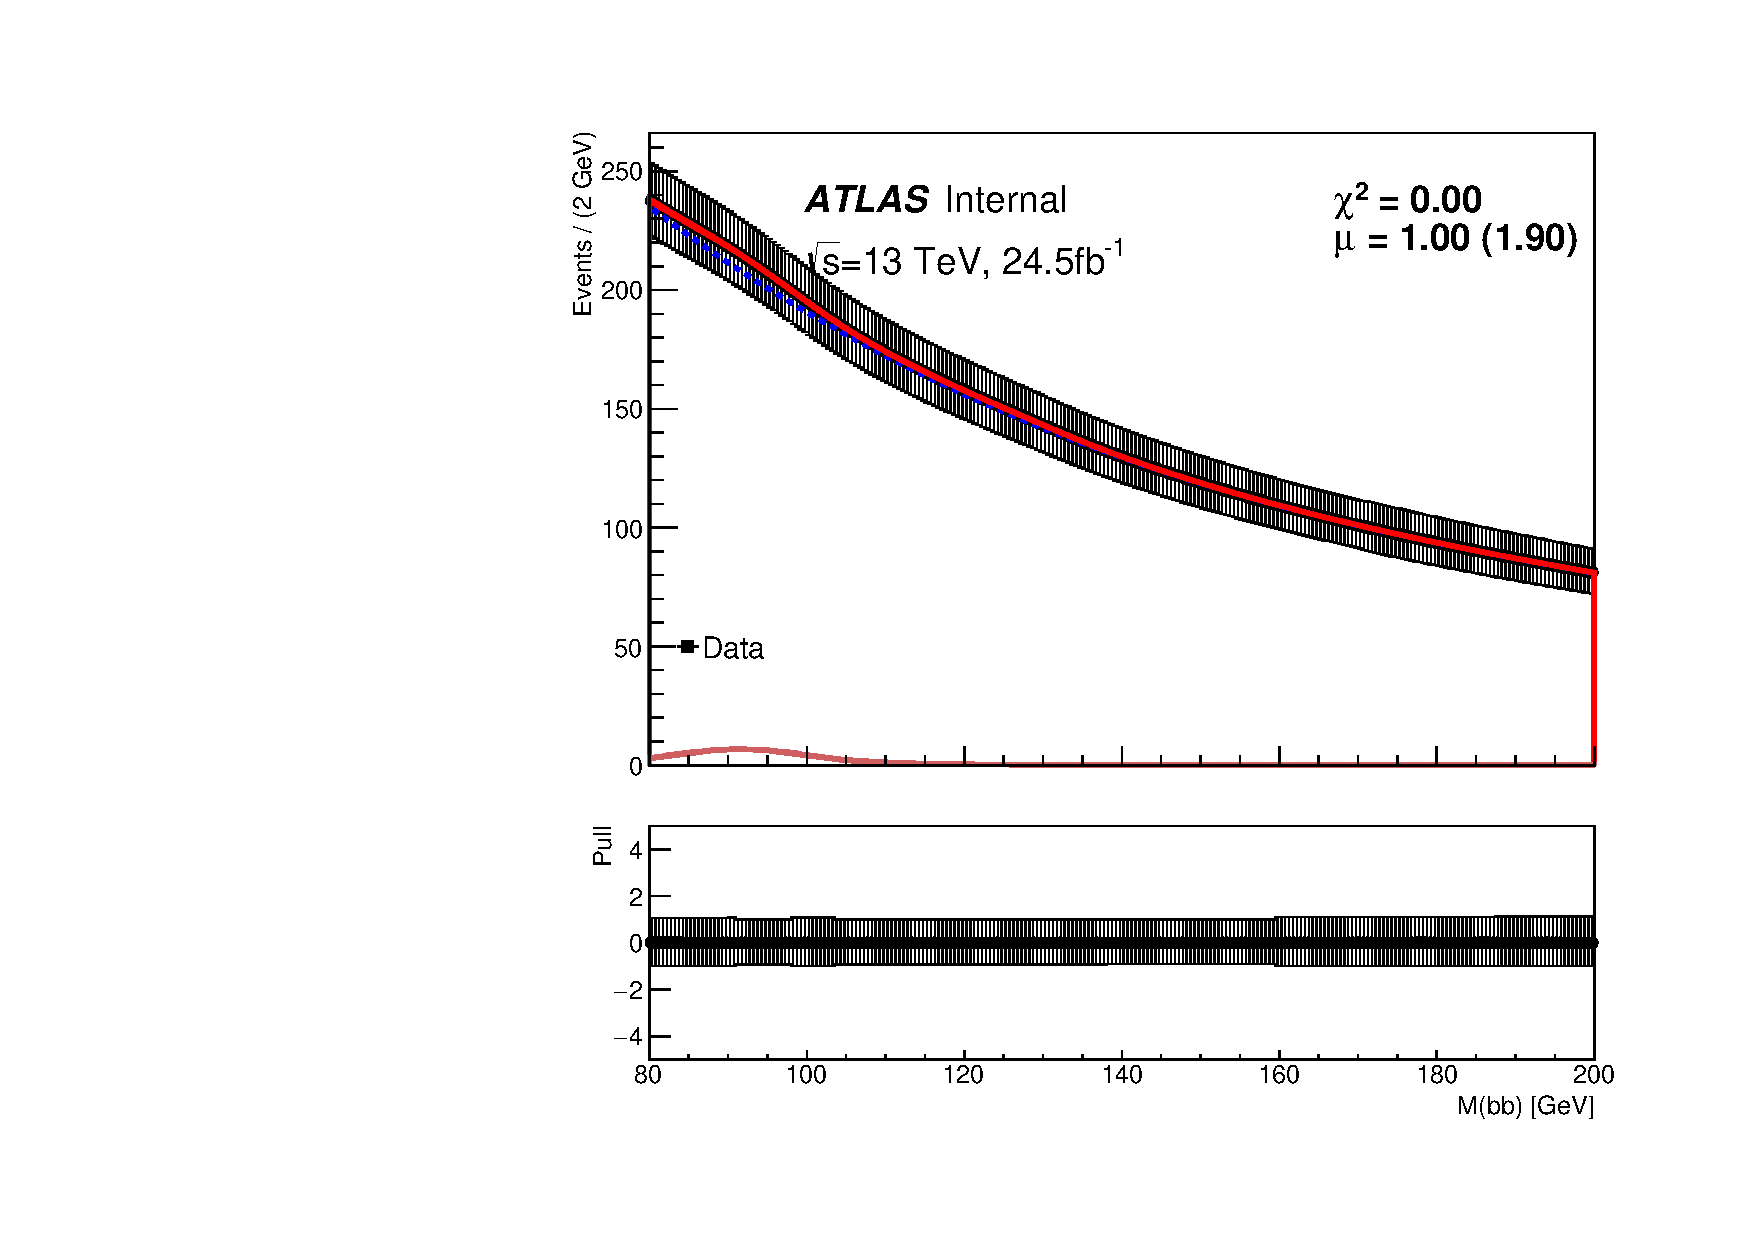
\includegraphics[width=0.48\textwidth]{figures_alt/Asimov_testVBF_ICHEP_4cen_SRI.pdf}
 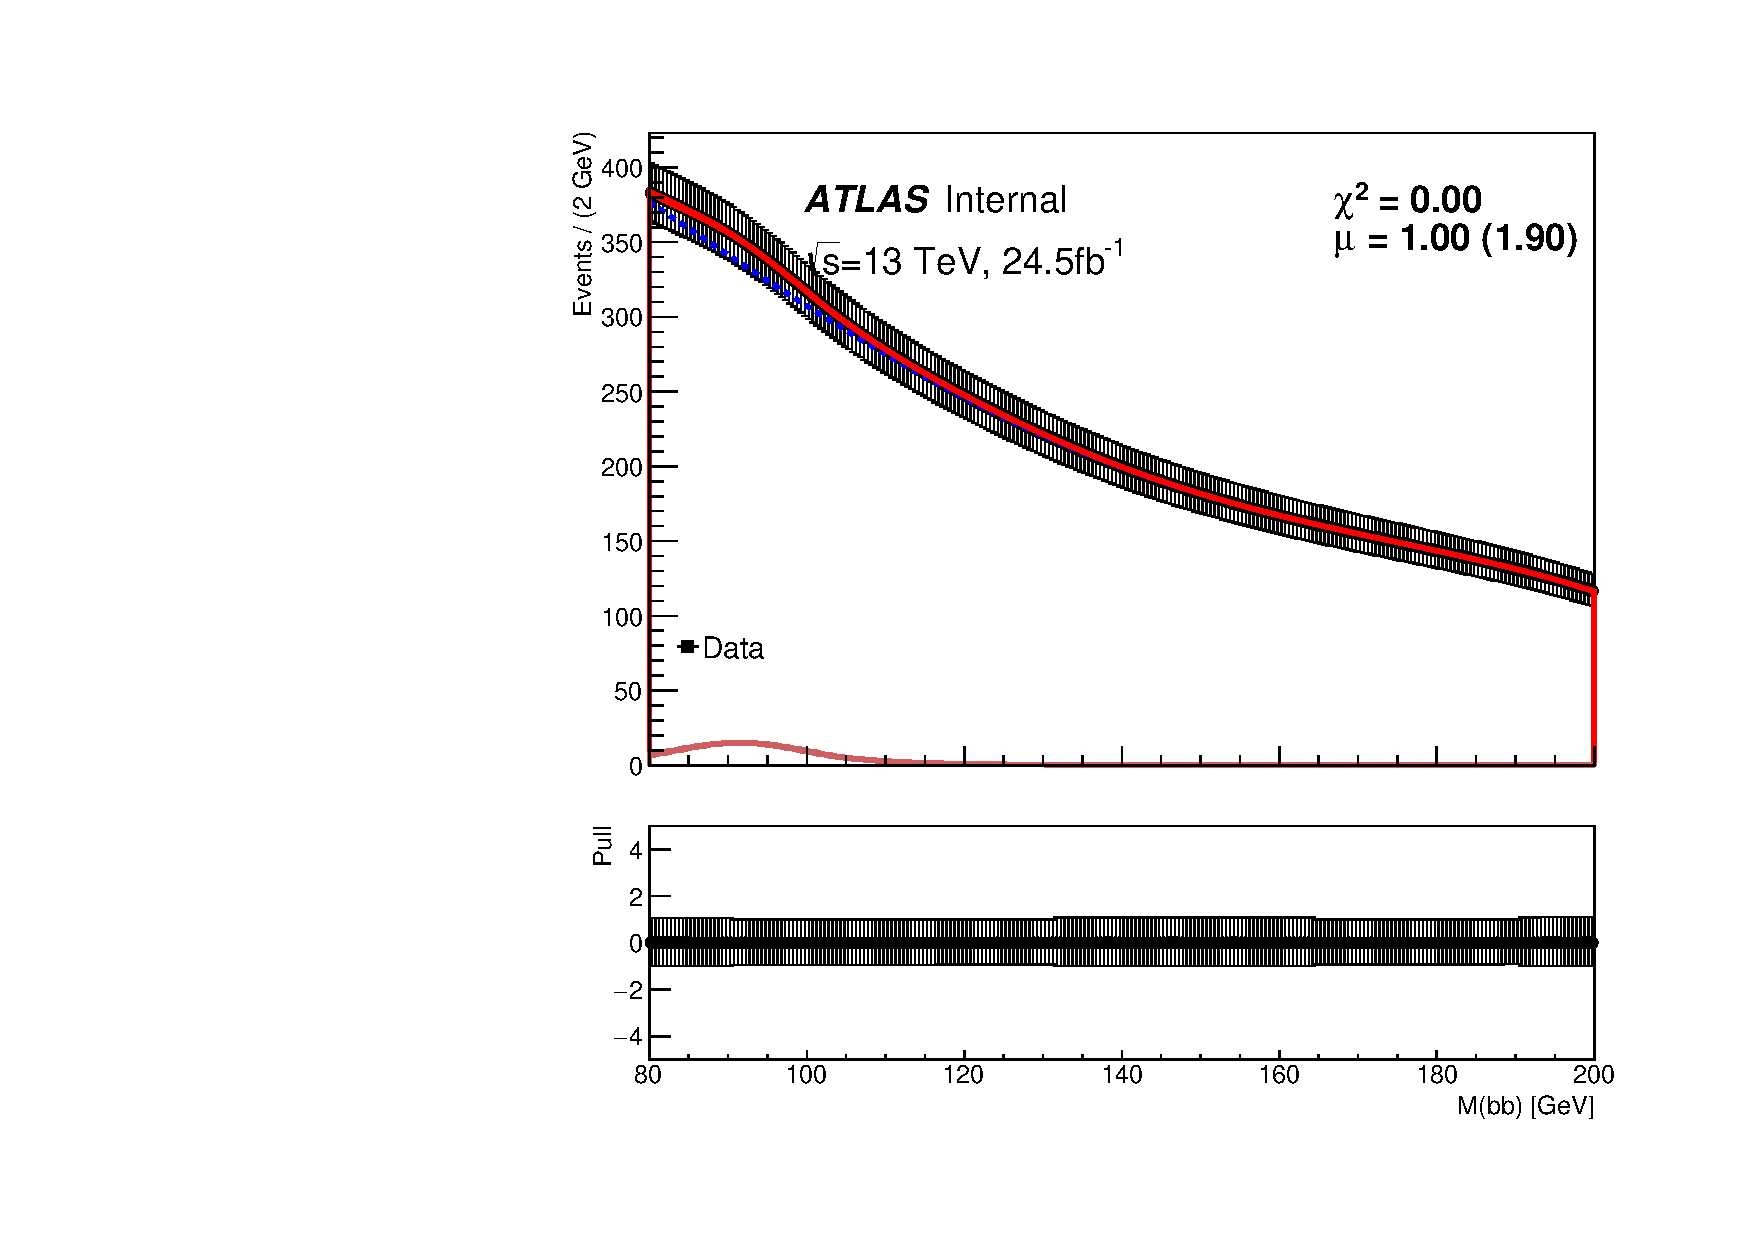
\includegraphics[width=0.48\textwidth]{figures_alt/Asimov_testVBF_ICHEP_4cen_SRII.pdf}
 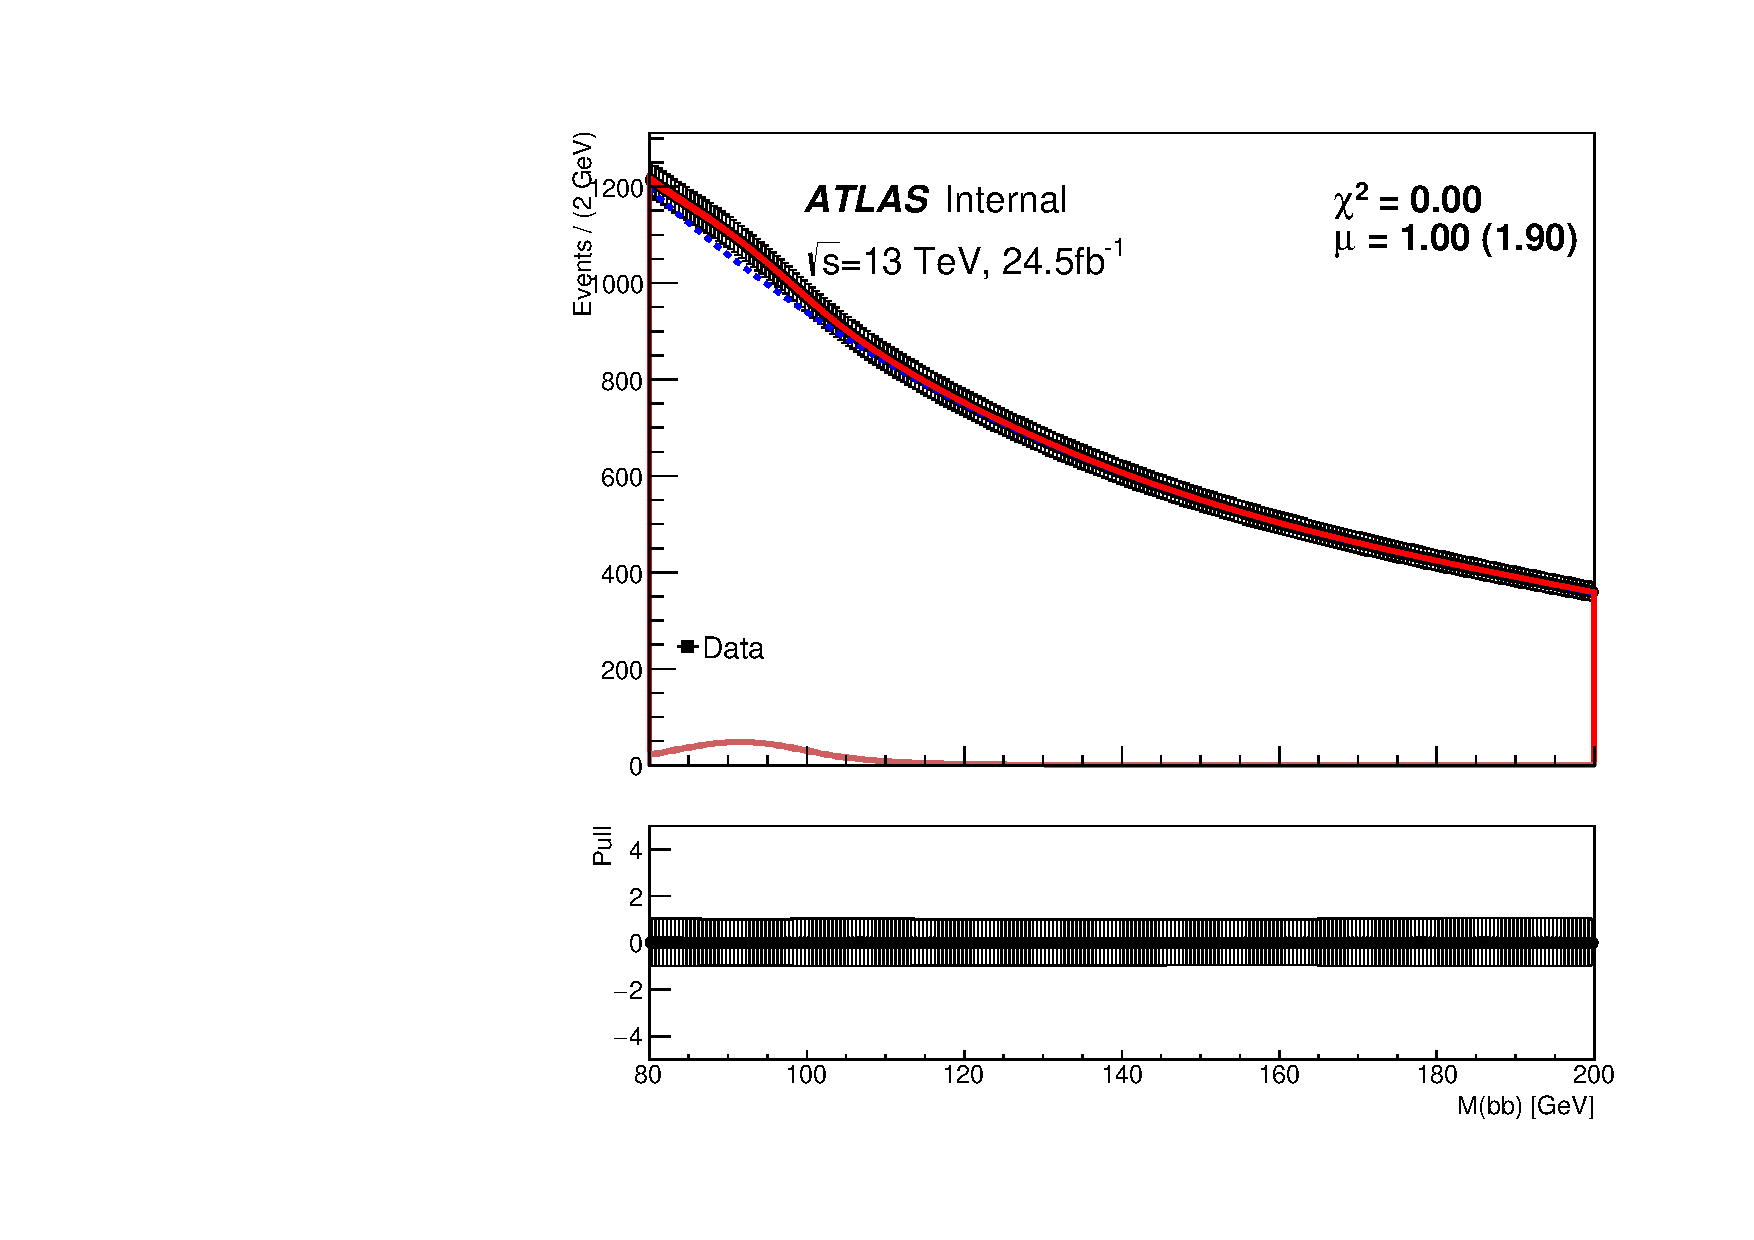
\includegraphics[width=0.48\textwidth]{figures_alt/Asimov_testVBF_ICHEP_4cen_SRIII.pdf}
 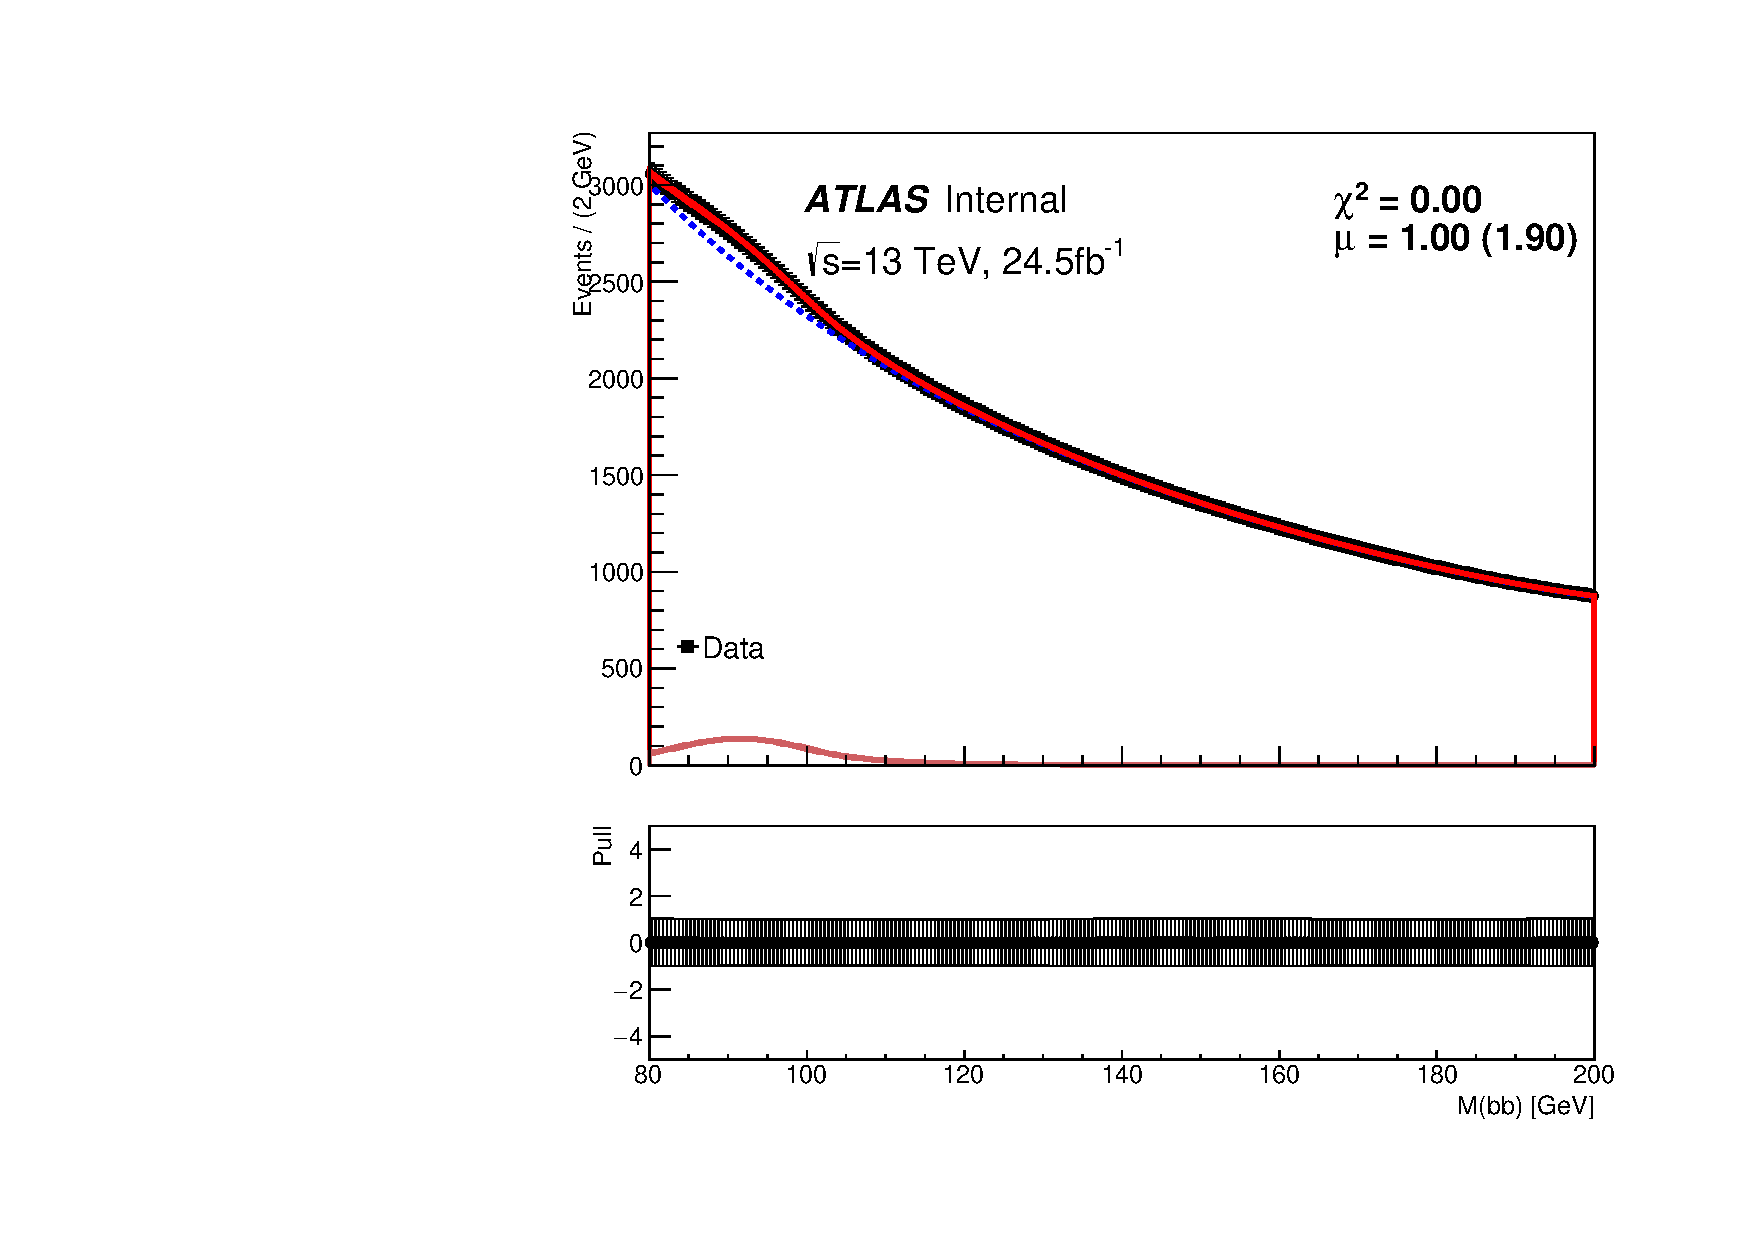
\includegraphics[width=0.48\textwidth]{figures_alt/Asimov_testVBF_ICHEP_4cen_SRIV.pdf}\\

\caption{Asymptotic Asimov fits for SR1 to SRIV for the \fourcentral channel.}
  \label{fig:4cenAsimov}
\end{figure}




%\subsubsection{Fit pseudo-data}
%
%Another check to test the robustness of the fit method as well as a check of the nuisance parameter pulls 
%is to use pseudo-data as close as possible to the real data. 
%For each signal region we construct the pseudo data by adding together three components:
%\begin{enumerate}
%\item Sideband ($80~\GeV <\Mbb<100$~\GeV~and $140~\GeV<\Mbb<200~\GeV$)
%\item Control region data in the Higgs mass window re-weighted linearly to the signal region using the fits described in Section~\ref{sec:nonres}.
%\item Signal MC scaled to Standard Model expectation for Higgs and \zjets{} production.
%\end{enumerate}
%
%The fit is performed simultaneously with both channels. We obtain closure as the best fitted signal strength is $\hat \mu = 0.56 \pm 1.15$. The fits are shown in Figures~\ref{fig:Fit_combined}. The post-fit impact of nuisance parameters and pulls for the simultaneous fit are shown in Figure~\ref{fig:pull}.  
%The parameters are defined as:
%\begin{itemize}
%\item nbkg\_X\_Y stands for background normalization in region X channel Y
%\item spurious stands for the strength of spurious signal
%OB\item  Lin\_X\_Y stands for the linear slope correction in region X channel Y
%\item x()2cen, x()4cen stands for Bernstein polynomial parameters in the \twocentral and \fourcentral channels respectively
%\item $\alpha\_z$ stands for the Z normalization NP
%\end{itemize} 
%The other parameter names follow the CP group definitions.  
%The largest contributions to the uncertainty on $\mu$ are from the background normalization and 
%control to signal region linear transfer factors. 
%%The only parameter pulled significantly is the $Z$ normalization, 
%%which is expected as we use a leading order generator for our $Z$+jets contribution.  
%%Further studies of the $Z$-contribution are discussed in Section~\ref{sec:znorm}.  
%
%\begin{figure}[htbp]
%  \centering
% 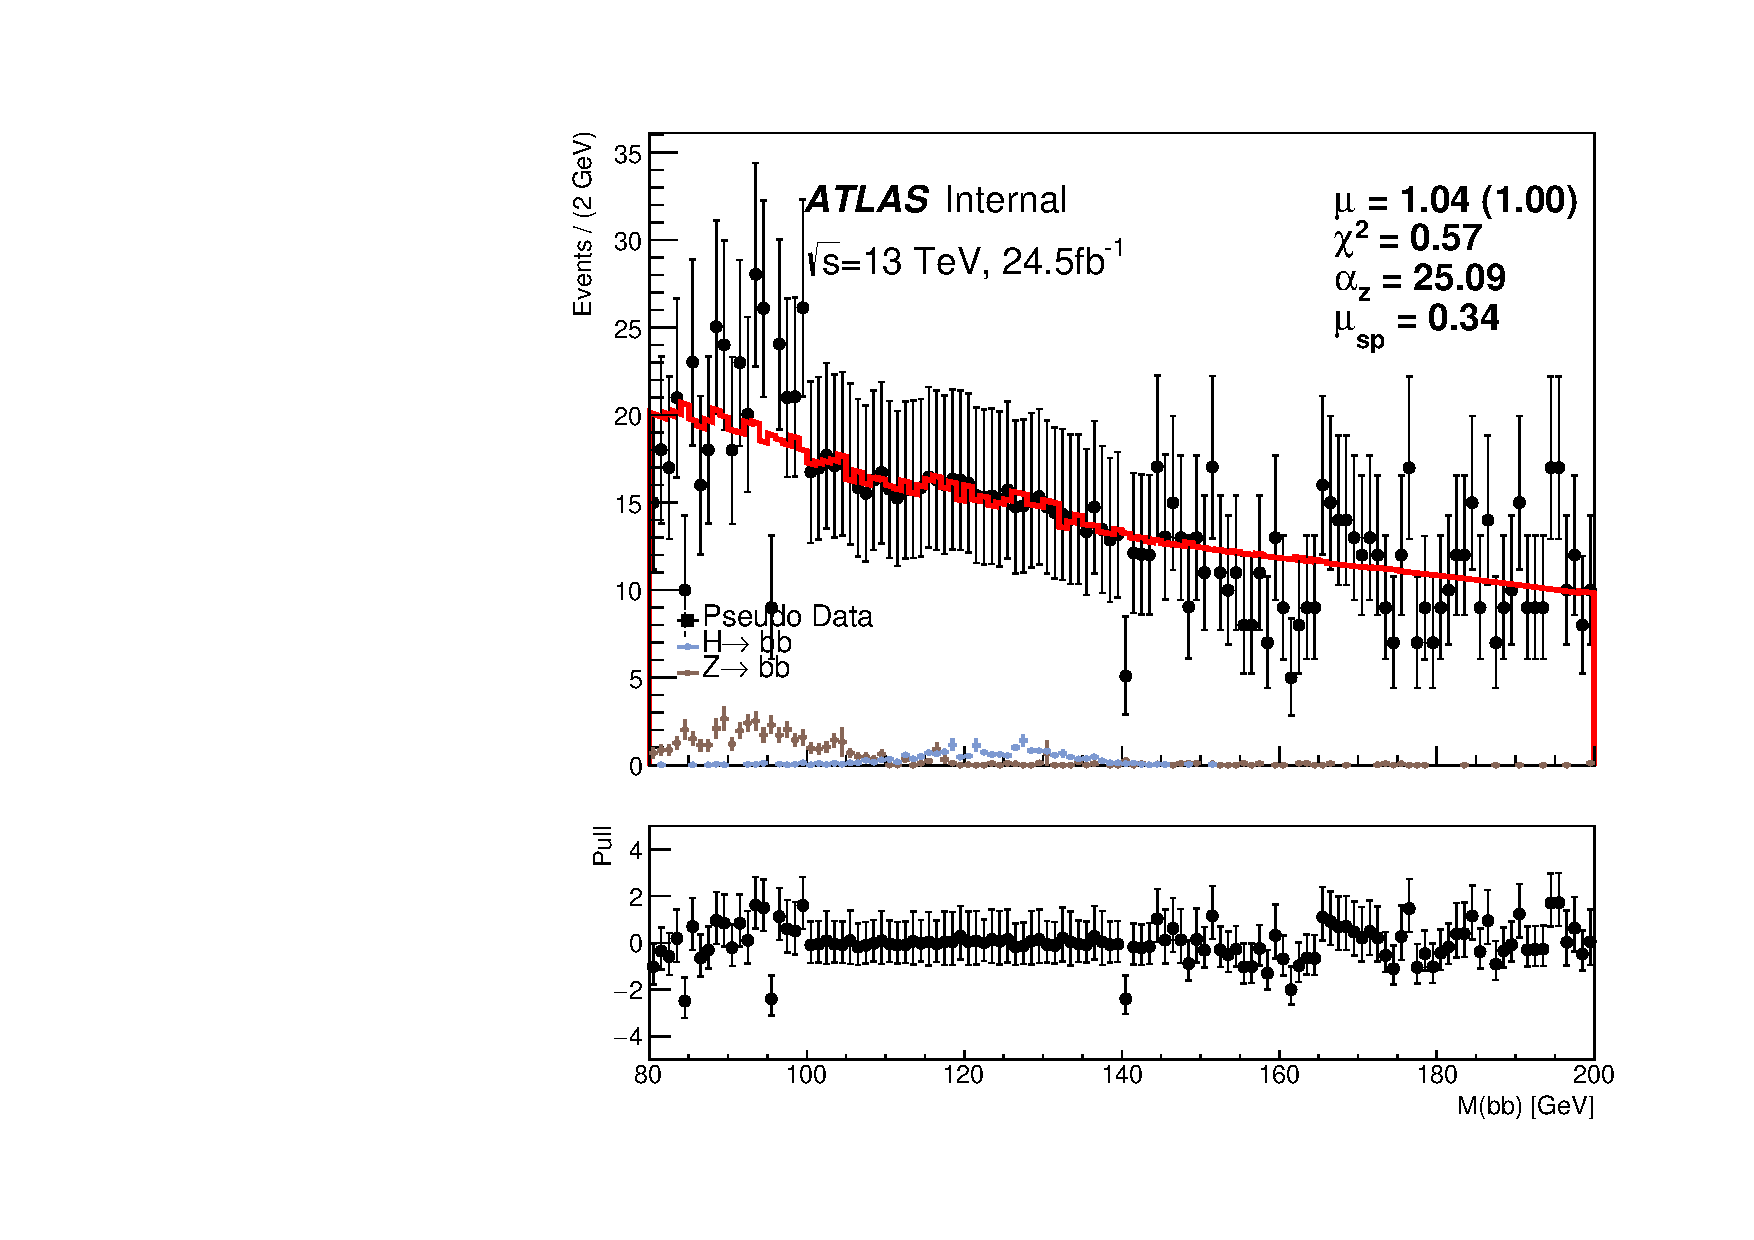
\includegraphics[width=0.32\textwidth]{figures/FitCombined/zcon_testVBF_ICHEP_2cen_SRI.pdf}
% 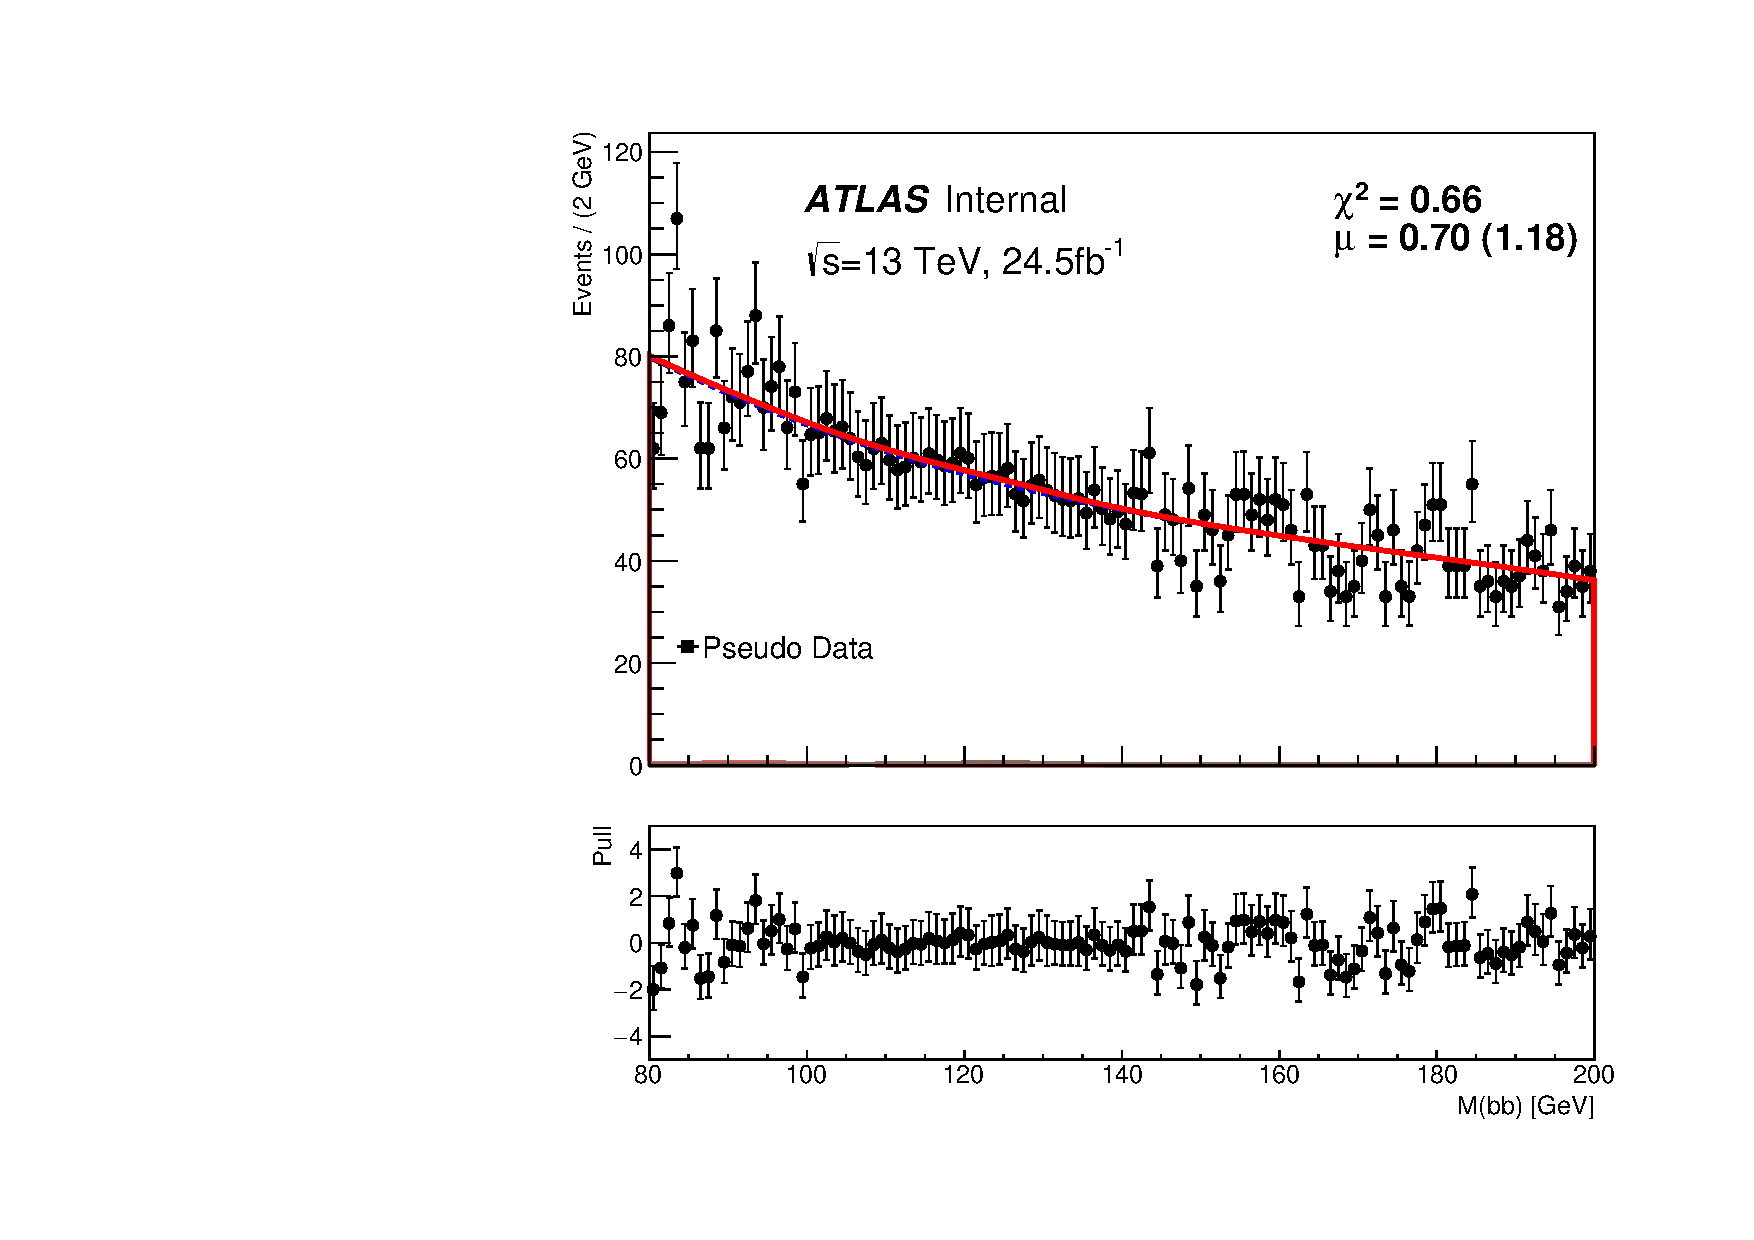
\includegraphics[width=0.32\textwidth]{figures/FitCombined/zcon_testVBF_ICHEP_2cen_SRII.pdf}
% 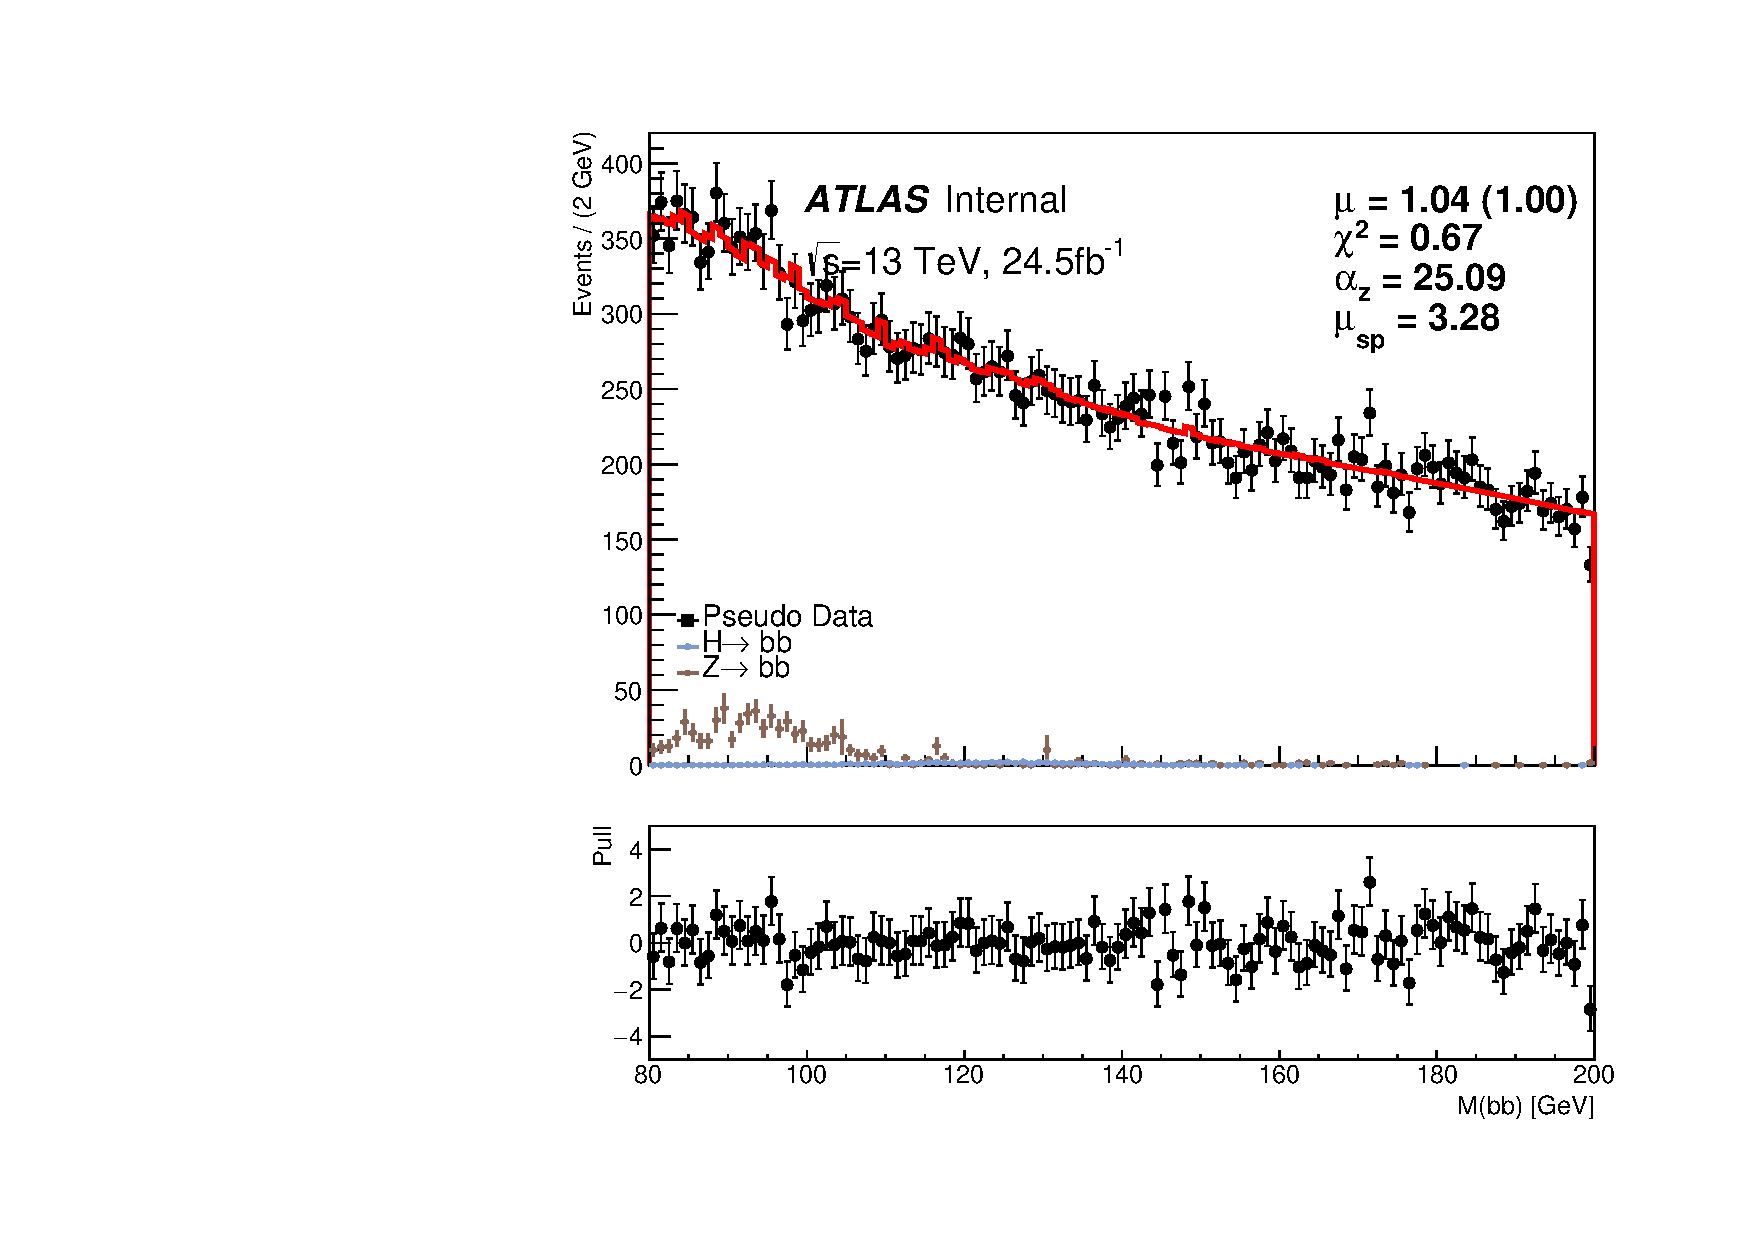
\includegraphics[width=0.32\textwidth]{figures/FitCombined/zcon_testVBF_ICHEP_2cen_SRIII.pdf}\\
% 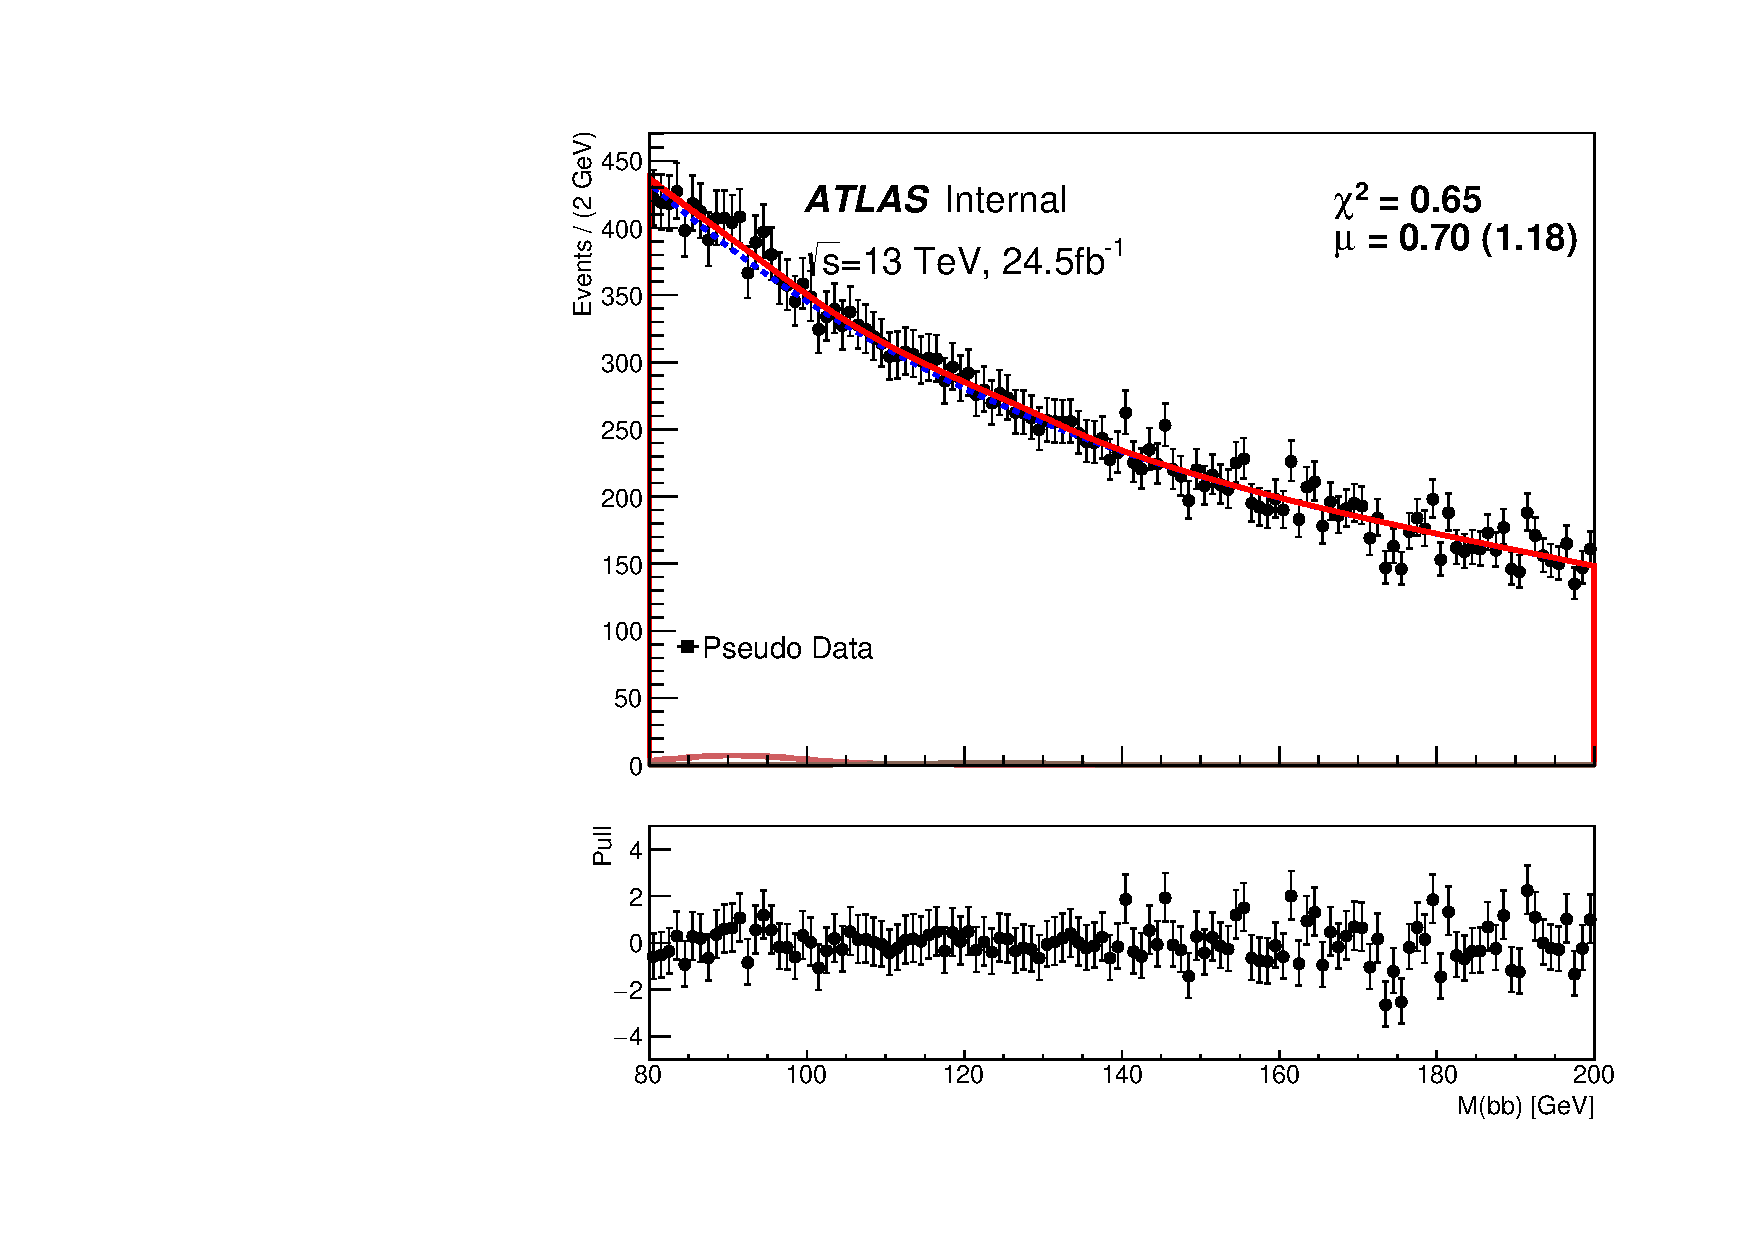
\includegraphics[width=0.32\textwidth]{figures/FitCombined/zcon_testVBF_ICHEP_4cen_SRI.pdf}
% 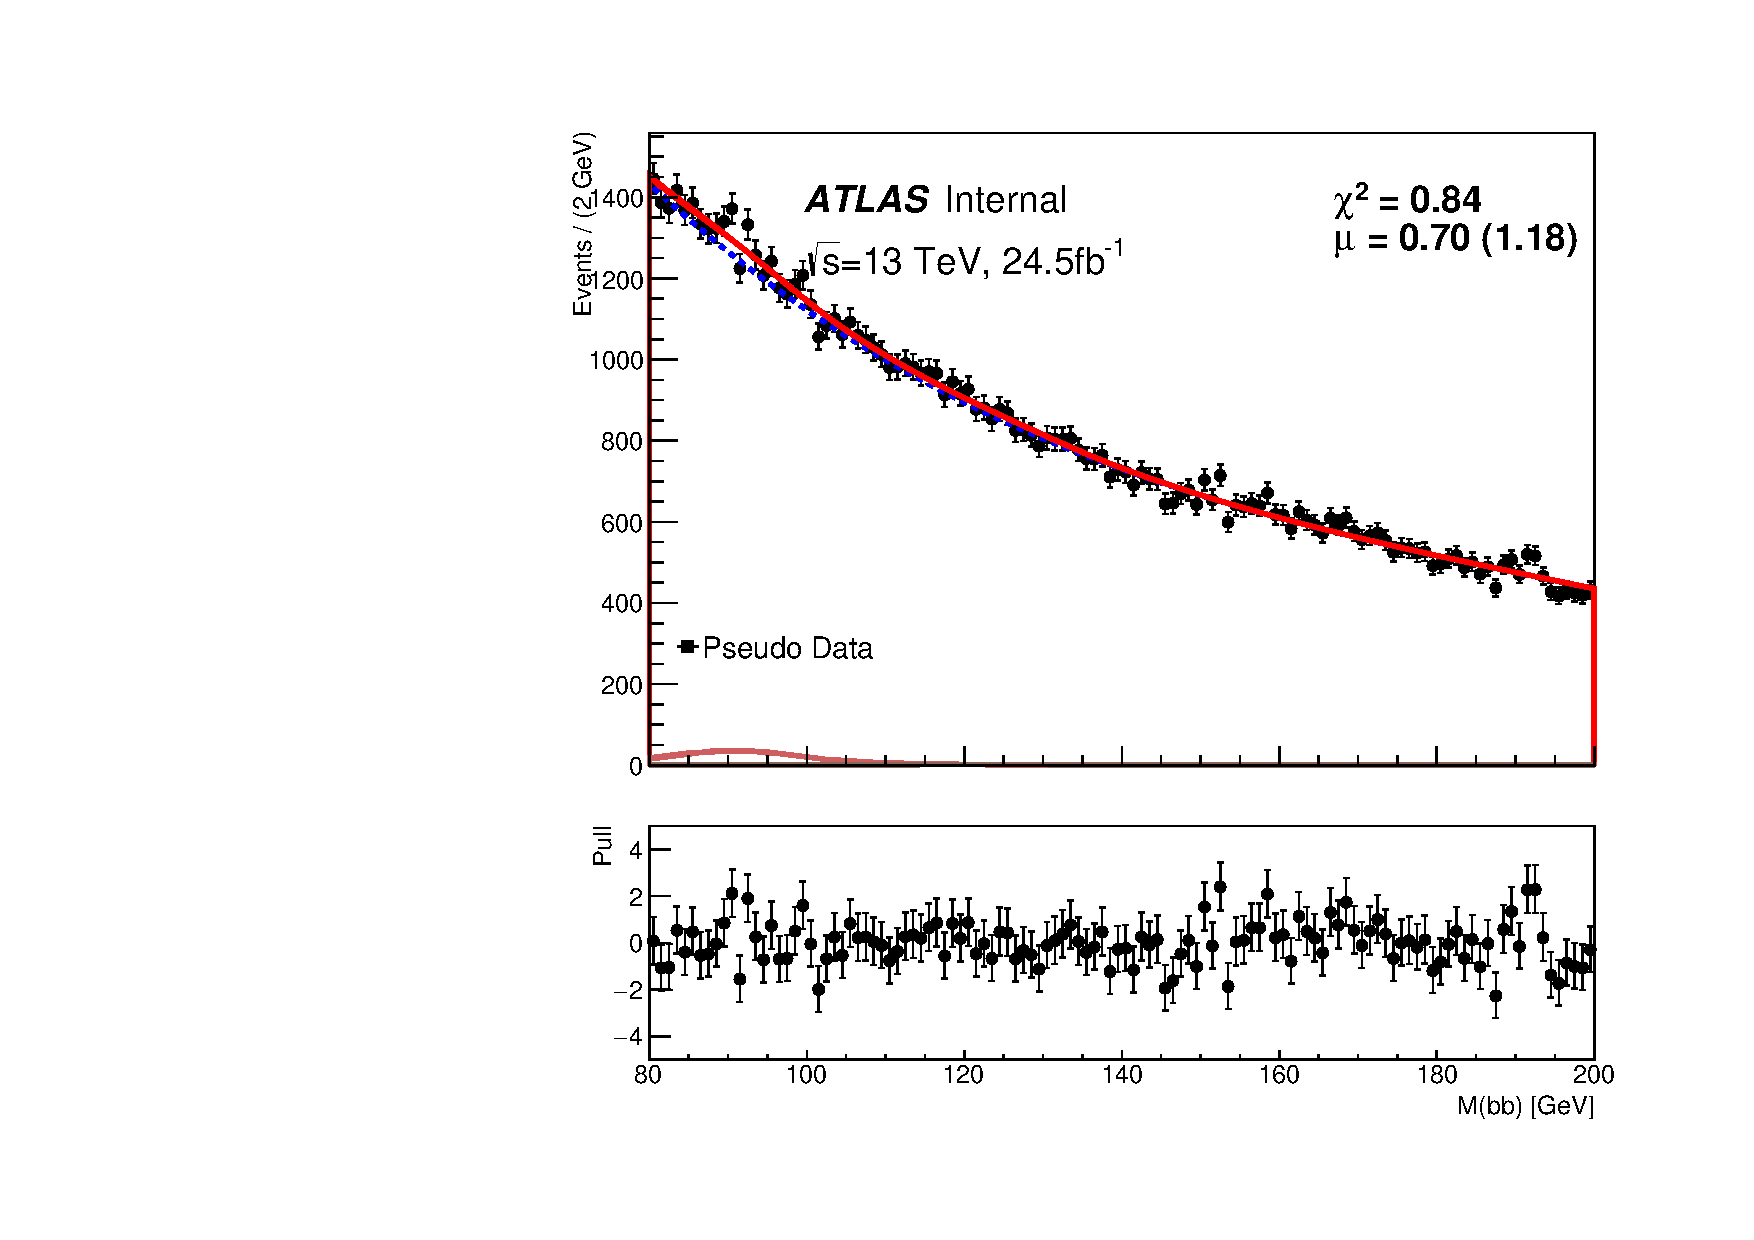
\includegraphics[width=0.32\textwidth]{figures/FitCombined/zcon_testVBF_ICHEP_4cen_SRII.pdf}\\
%
%\caption{Pseudo data fit for both channels. Fits from SR I to SR III (SR II) for 2 central (top) and 4 central (bottom) are shown.}
%  \label{fig:Fit_combined}
%\end{figure}


\begin{figure}[htbp]
  \centering
 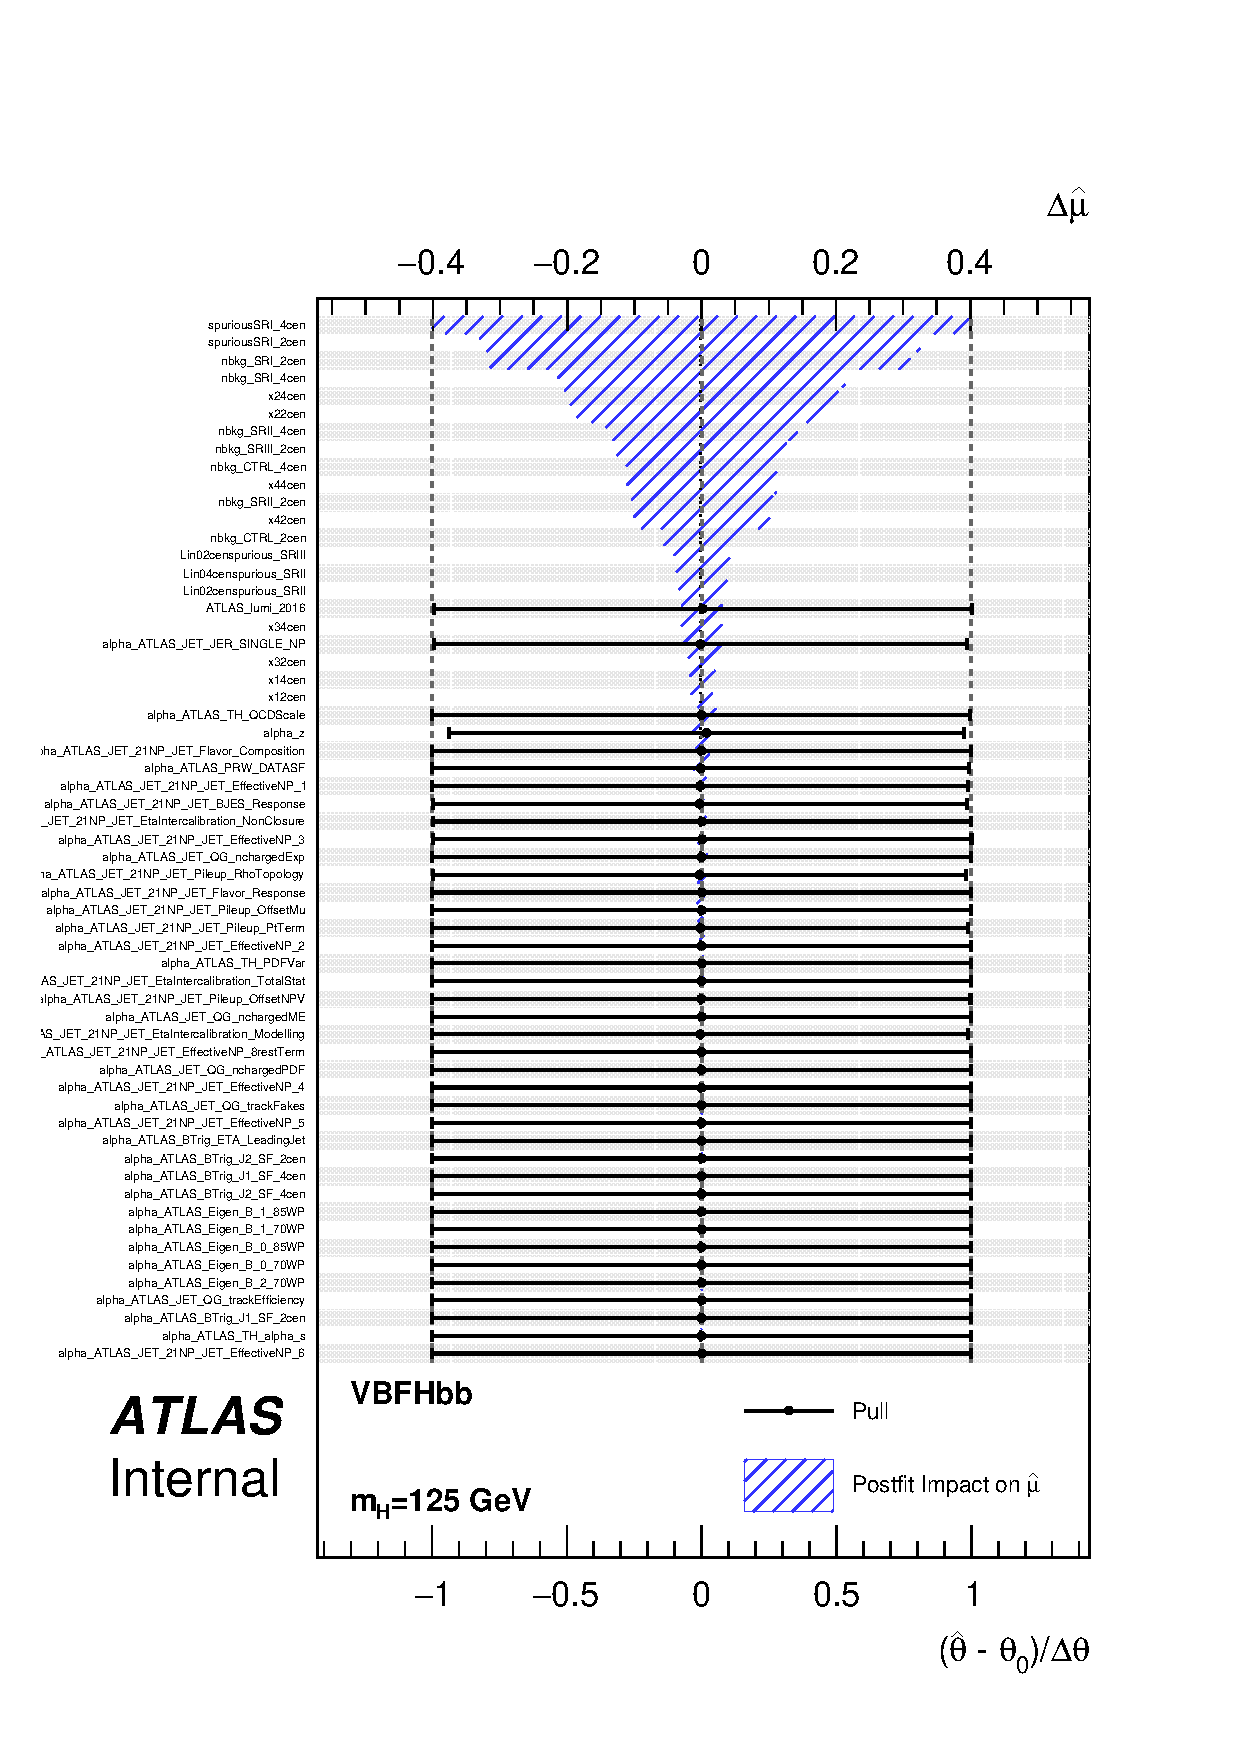
\includegraphics[width=0.9\textwidth]{figures_alt/VBFHbb_pulls_125_Asimov.pdf}

\caption{Nuisance parameter post-fit impact and pulls are plotted for the simultaneous Asimov fit of two channels. The background normalizations are pre-fixed as "nbkg''. The spurious signal size are pre-fixed as "spurious''. The background parameterizations are pre-fixed as  "x*2cen'' for 2 central channel and "x*4cen'' for 4 central channel. The experimental uncertainties follow the standard ATLAS naming. The dominant systematics are the spurious signal and background parameters.}
  \label{fig:pull_asimov}
\end{figure}


\begin{figure}[htbp]
  \centering
 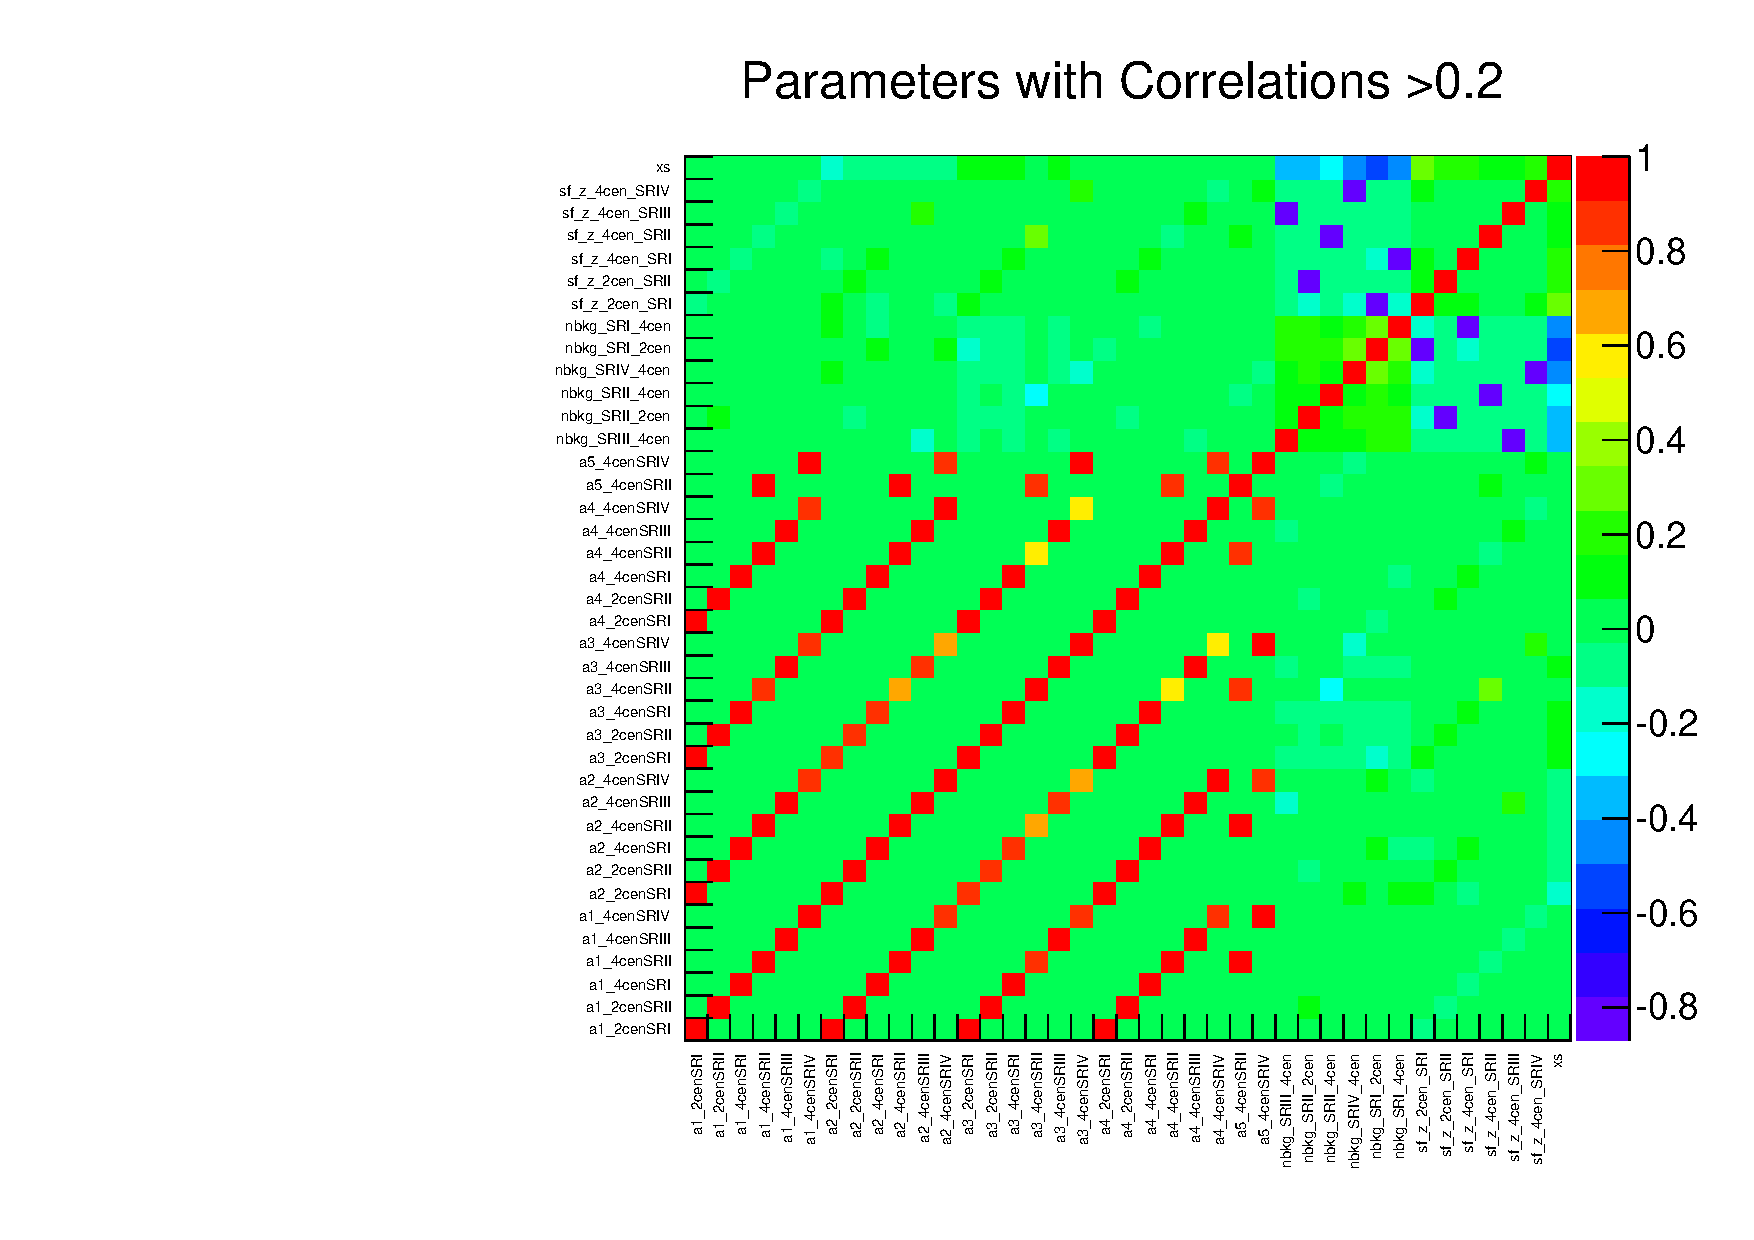
\includegraphics[width=0.95\textwidth]{figures_alt/Correlation.pdf}

\caption{Nuisance parameter correlation for Asimov fit}
  \label{fig:corr_asimov}
\end{figure}


%\begin{figure}[htbp]
%  \centering
% 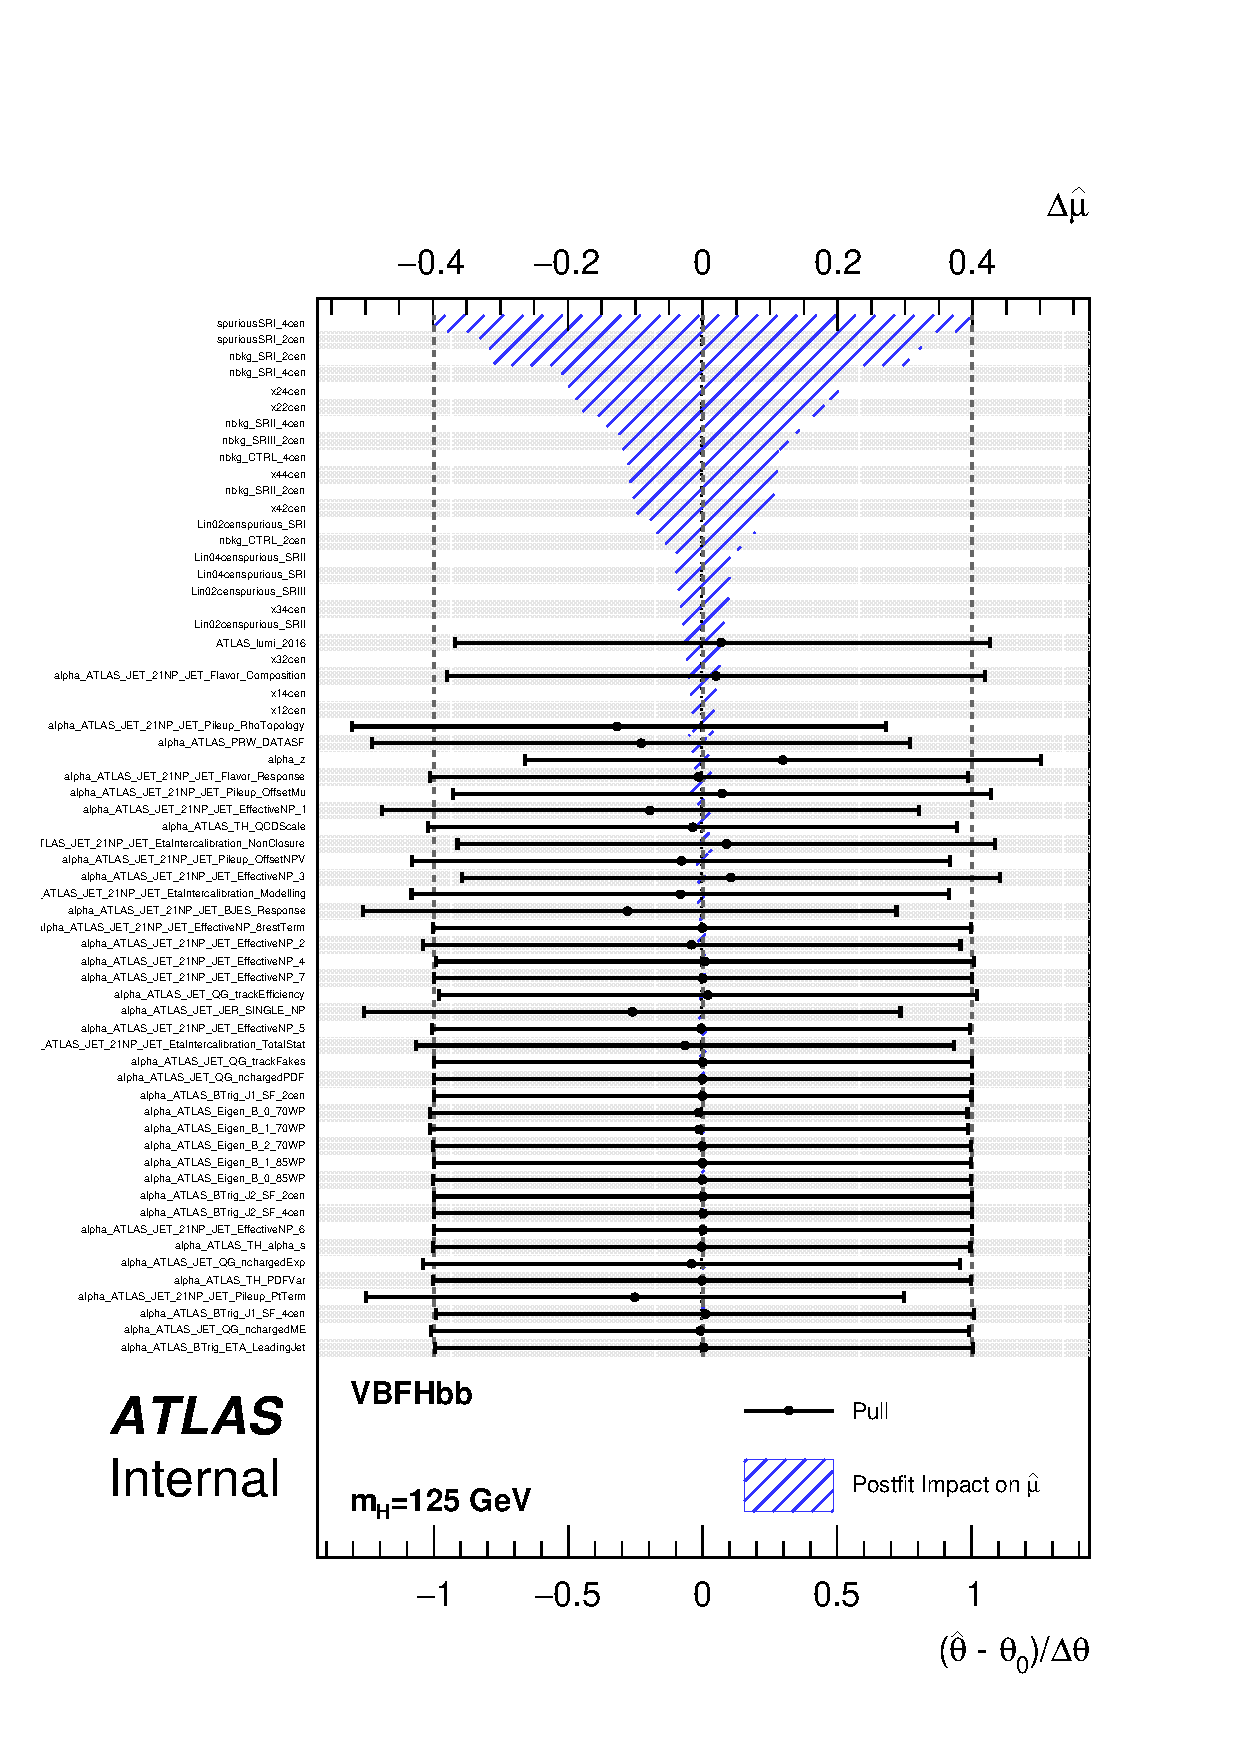
\includegraphics[width=0.9\textwidth]{figures/FitCombined/VBFHbb_pulls_125.pdf}
%
%\caption{Nuisance parameter post-fit impact and pulls are plotted for the simultaneous fit of two channels for the pseudodata. The background normalizations are pre-fixed as "nbkg''. The Linear transfer function are pre-fixed as "Lin''. The spurious signal size are pre-fixed as "spurious''. The background parameterizations are pre-fixed as  "x()2cen'' for 2 central channel and "x()4cen'' for 4 central channel. The JES and JER parameters are prefixed by ``alpha\_ATLAS\_JET".  The \btagging parameters are prefixed by ``alpha\_ATLAS\_eigen". The most significant contribution to the uncertainty of signal strength comes from background normalization.}
%  \label{fig:pull}
%\end{figure}
